\documentclass[lang = cn, scheme = chinese, thmcnt = section]{elegantbook}
% elegantbook      设置elegantbook文档类
% lang = cn        设置中文环境
% scheme = chinese 设置标题为中文
% thmcnt = section 设置计数器


%% 1.封面设置

\title{数学分析 - 陈纪修 - 笔记}                % 文档标题

\author{若水}                        % 作者

\myemail{ethanmxzhou@163.com}       % 邮箱

\homepage{helloethanzhou.github.io} % 主页

\date{\today}                       % 日期

\logo{PiCreatures_happy.pdf}        % 设置Logo

\cover{阿基米德螺旋曲线.pdf}          % 设置封面图片

% 修改标题页的色带
\definecolor{customcolor}{RGB}{135, 206, 250} 
% 定义一个名为customcolor的颜色,RGB颜色值为(135, 206, 250)

\colorlet{coverlinecolor}{customcolor}     % 将coverlinecolor颜色设置为customcolor颜色

%% 2.目录设置
\setcounter{tocdepth}{3}  % 目录深度为3

%% 3.引入宏包
\usepackage[all]{xy}
\usepackage{bbm, svg, graphicx, float, extpfeil, amsmath, amssymb, mathrsfs, mathalpha, hyperref, centernot, physics}


%% 4.定义命令
\newcommand{\N}{\mathbb{N}}            % 自然数集合
\newcommand{\R}{\mathbb{R}}            % 实数集合
\newcommand{\C}{\mathbb{C}}  		   % 复数集合
\newcommand{\Q}{\mathbb{Q}}            % 有理数集合
\newcommand{\Z}{\mathbb{Z}}            % 整数集合
\newcommand{\sub}{\subset}             % 包含
\newcommand{\im}{\text{im }}           % 像
\newcommand{\lang}{\langle}            % 左尖括号
\newcommand{\rang}{\rangle}            % 右尖括号
\newcommand{\bs}{\boldsymbol}          % 向量加黑
% \newcommand{\dd}{\mathrm{d}}           % 微分d
\newcommand{\dis}{\displaystyle}
\newcommand{\Int}{\int\limits}
\newcommand{\IInt}{\iint\limits}
\newcommand{\IIInt}{\iiint\limits}
\newcommand{\ee}[1]{\mathrm{e}^{#1}}
\newcommand{\function}[5]{
	\begin{align*}
		#1:\begin{aligned}[t]
			#2 &\longrightarrow #3\\
			#4 &\longmapsto #5
		\end{aligned}
	\end{align*}
}                                     % 函数

\newcommand{\lhdneq}{%
	\mathrel{\ooalign{$\lneq$\cr\raise.22ex\hbox{$\lhd$}\cr}}} % 真正规子群

\newcommand{\rhdneq}{%
	\mathrel{\ooalign{$\gneq$\cr\raise.22ex\hbox{$\rhd$}\cr}}} % 真正规子群

\begin{document}
	
	\maketitle       % 创建标题页
	
	\frontmatter     % 开始前言部分
	
	\chapter*{致谢}
	
	\markboth{致谢}{致谢}
	
	\vspace*{\fill}
	\begin{center}
		
		\large{感谢 \textbf{ 勇敢的 } 自己}
		
	\end{center}
	\vspace*{\fill}
	
	\tableofcontents % 创建目录
	
	\mainmatter      % 开始正文部分

\chapter{实数体系的构造}

\section{Peano公理}

\subsection{相等}

\begin{definition}{等价关系}
	称关系$\sim$为集合$X$上的等价关系,如果成立如下命题。
	\begin{enumerate}
		\item 自反性:$\forall x\in X,\quad x \sim x$
		\item 对称性:$\forall x,y\in X,\quad (x\sim y\implies y\sim x)$
		\item 传递性:$\forall x,y,z\in X,\quad ((x\sim y)\wedge(y\sim z)\implies x\sim z)$
	\end{enumerate}
\end{definition}

\begin{definition}{相等}
	定义集合$X$上的相等为一种等价关系,记作$=$。
\end{definition}

\subsection{自然数}

\begin{axiom}{Peano公理}{Peano公理}
	\begin{enumerate}
		\item $0\in\N$
		\item $\forall n\in\N,\quad (n\in\N\implies n*\in\N)$
		\item $\forall n\in\N,\quad n*\ne 0$
		\item $\forall m,n\in\N,\quad (m=n\iff m*=n*)$
		\item 对于命题$P:\N\to\text{Bool}$,如果
		\begin{align*}
			& P(0)=\text{True}\\
			& \forall n\in\N^*,\quad (P(n)=\text{True}\implies P(n*)=\text{True})
		\end{align*}
		那么
		$$
		\forall n\in\N^*,\quad P(n)=\text{True}
		$$
	\end{enumerate}
\end{axiom}

\begin{definition}{自然数集}
	称成立Peano公理的集合$\N$为自然数集。
\end{definition}

\section{加法}

\subsection{加法}

\begin{definition}{加法}
	\begin{align*}
		& \forall n\in\N,\quad n+0\coloneqq n\\
		& \forall m,n\in\N,\quad m+(n*)\coloneqq (m+n)*
	\end{align*}
\end{definition}

\begin{proposition}{加法的性质}
	\begin{enumerate}
		\item 加法交换律:
		$$
		\forall m,n\in\N,\quad m+n=n+m
		$$
		\item 加法结合律:
		$$
		\forall l,m,n\in\N,\quad (l+m)+n=l+(m+n)
		$$
		\item 消去律:
		$$
		\forall l,m,n\in\N,\quad (l+m=l+n\implies m=n)
		$$
	\end{enumerate}
\end{proposition}

\subsection{自然数的序}

\begin{definition}{正自然数}
	定义正自然数集为$\N^*=\N\setminus\{0\}$。
\end{definition}

\begin{proposition}
	$$
	n\in\N^*\iff
	\exists!m\in\N,m*=n
	$$
\end{proposition}

\begin{definition}{自然数的序}
	\begin{enumerate}
		\item 对于自然数$m,n\in\N$,称$m \ge n$,如果存在自然数$l\in\N$,使得成立$m=l+n$。
		\item 对于自然数$m,n\in\N$,称$m > n$,如果存在正自然数$l\in\N^*$,使得成立$m=l+n$。
	\end{enumerate}
\end{definition}

\begin{proposition}{序的性质}
	\begin{enumerate}
		\item 自反性:$\forall n\in\N,\quad n \ge n$
		\item 传递性:$\forall l,m,n\in\N,\quad (l\ge m)\wedge(m\ge n)\implies l\ge n$
		\item 反称性:$\forall m,n\in\N,\quad (m\ge n)\wedge(n\ge m)\implies m=n$
	\end{enumerate}
\end{proposition}

\begin{theorem}{序的三歧性}
	对于自然数$n\in\N$,以下三命题有且仅有其一为真。
	\begin{enumerate}
		\item $n=0$
		\item $n>0$
		\item $n<0$
	\end{enumerate}
\end{theorem}

\begin{theorem}{强数学归纳法}
	对于命题$P:\N\to\text{Bool}$,如果
	\begin{align*}
		& P(0)=\text{True}\\
		& \forall n\in \N,\quad ((\forall m\in \N,\quad (m< n\implies P(m)=\text{True}))\implies P(n)=\text{True})
	\end{align*}
	那么
	$$
	\forall n\in\N^*,\quad P(n)=\text{True}
	$$
\end{theorem}

\section{乘法}

\begin{definition}{乘法}
	\begin{align*}
		& \forall n\in\N,\quad n\times 0\coloneqq 0\\
		& \forall m,n\in\N,\quad m\times (n*)\coloneqq (m\times n)+m
	\end{align*}
\end{definition}

\begin{proposition}{乘法的性质}
	\begin{enumerate}
		\item 乘法交换律:
		$$
		\forall m,n\in\N,\quad m\times n=n\times m
		$$
		\item 乘法结合律:
		$$
		\forall l,m,n\in\N,\quad (l\times m)\times n=l\times (m\times n)
		$$
		\item 保序性:
		$$
		\forall l,m,n\in\N,\quad (m>n)\wedge(l>0)\implies l\times m>l\times n
		$$
		\item 消去律:
		$$
		\forall l,m,n\in\N,\quad (l\times m=l\times n)\wedge(l>0)\implies m=n
		$$
	\end{enumerate}
\end{proposition}

\section{整数}

\subsection{整数}

\begin{definition}{整数}
	对于$m,n\in\N$,定义$m\ominus n$为整数。
\end{definition}

\begin{definition}{整数的相等}
	对于$a,b,c,d\in\N$,称$a\ominus b=c\ominus d$,如果$a+d=c+b$。
\end{definition}

\begin{definition}{整数集}
	整数全体构成整数集$\Z$。
\end{definition}

\begin{definition}{整数的加法}
	$$
	\forall a,b,c,d\in\N,\quad (a\ominus b)+(c\ominus d)\coloneqq (a+c)\ominus(b+d)
	$$
\end{definition}

\begin{definition}{整数的乘法}
	$$
	\forall a,b,c,d\in\N,\quad (a \ominus b) \times (c \ominus d)\coloneqq (a\times c+b\times d)\ominus(a\times d+b\times c)
	$$
\end{definition}

\begin{definition}{相反数}
	对于$m,n\in\N$,定义$m\ominus n$的相反数为$-(m \ominus n)\coloneqq n \ominus m$。
\end{definition}

\begin{definition}{整数的减法}
	$$
	\forall a,b,c,d\in\N,\quad (a \ominus b)-(c \ominus d)\coloneqq (a \ominus b)+(-(c \ominus d))
	$$
\end{definition}

\subsection{整数的序}

\begin{definition}{整数的序}
	\begin{enumerate}
		\item 对于整数$m,n\in\Z$,称$m \ge n$,如果存在自然数$l\in\N$,使得成立$m=l+n$。
		\item 对于整数$m,n\in\Z$,称$m > n$,如果存在正自然数$l\in\N^*$,使得成立$m=l+n$。
	\end{enumerate}
\end{definition}

\begin{definition}{正整数,负整数,非负整数}
	\begin{enumerate}
		\item 称整数$n\in\Z$为正整数,如果$n>0$。
		\item 称整数$n\in\Z$为负整数,如果$n<0$。
		\item 称整数$n\in\Z$为非负整数,如果$n\ge 0$。
	\end{enumerate}
\end{definition}

\begin{proposition}{序的性质}
	\begin{enumerate}
		\item 自反性:$\forall n\in\Z,\quad n \ge n$
		\item 传递性:$\forall l,m,n\in\Z,\quad (l\ge m)\wedge(m\ge n)\implies l\ge n$
		\item 反称性:$\forall m,n\in\Z,\quad (m\ge n)\wedge(n\ge m)\implies m=n$
	\end{enumerate}
\end{proposition}

\begin{theorem}{序的三歧性}
	对于整数$m,n\in\Z$,以下三命题有且仅有其一为真。
	\begin{enumerate}
		\item $m=n$
		\item $m>n$
		\item $m<n$
	\end{enumerate}
\end{theorem}

\section{比例数}

\subsection{比例数}

\begin{definition}{比例数}
	对于$m,n\in\N$且$n\ne 0$,定义$m\oslash n$为比例数。
\end{definition}

\begin{definition}{比例数的相等}
	对于$a,b,c,d\in\N$且$b,d\ne 0$,称$a\oslash  b=c\oslash  d$,如果$a\times d=b\times c$。
\end{definition}

\begin{definition}{比例数集}
	比例数全体构成比例数集$\Q$。
\end{definition}

\subsection{比例数的四则运算}

\begin{definition}{比例数的加法}
	$$
	\forall (a,b,c,d\in\N)\wedge (b,d\ne 0),\quad (a \oslash b)+(c \oslash d)\coloneqq (a\times d+b\times c)\oslash(b\times d)
	$$
\end{definition}

\begin{definition}{比例数的乘法}
	$$
	\forall (a,b,c,d\in\N)\wedge (b,d\ne 0),\quad 
	(a \oslash b)\times(c \oslash d)\coloneqq (a\times c)\oslash(b\times d)
	$$
\end{definition}

\begin{definition}{比例数的负数}
	$$
	\forall (a,b\in\N)\wedge (b\ne 0),\quad 
	-(a\oslash b)\coloneqq (-a)\oslash b
	$$
\end{definition}

\begin{definition}{比例数的减法}
	$$
	\forall (a,b,c,d\in\N)\wedge (b,d\ne 0),\quad 
	(a \oslash b)-(c \oslash d)\coloneqq (a \oslash b)+(-(c \oslash d))
	$$
\end{definition}

\begin{definition}{比例数的倒数}
	$$
	\forall (a,b\in\N)\wedge (a,b\ne 0),\quad 
	(a\oslash b)^{-1}\coloneqq b \oslash a
	$$
\end{definition}

\begin{definition}{比例数的除法}
	$$
	\forall (a,b,c,d\in\N)\wedge (b,c,d\ne 0),\quad 
	(a \oslash b)\divisionsymbol (c \oslash d)\coloneqq 
	(a \oslash b)\times (c \oslash d)^{-1}
	$$
\end{definition}

\subsection{比例数的序}

\begin{definition}{正比例数}
	称比例数$x\in\Q$为正比例数,如果存在正自然数$m,n\in N^*$,使得成立$x=m \oslash n$。
\end{definition}

\begin{definition}{非负比例数}
	称比例数$x\in\Q$为非负比例数,如果或$x=0$,或$x$为正比例数。
\end{definition}

\begin{definition}{比例数的序}
	\begin{enumerate}
		\item 对于比例数$x,y\in\Q$,称$x \ge y$,如果存在非负比例数$z\in\Q$,使得成立$x=y+z$。
		\item 对于整数$x,y\in\N$,称$x>y$,如果存在正比例数$z\in\Q$,使得成立$x=y+z$。
	\end{enumerate}
\end{definition}

\begin{proposition}{序的性质}
	\begin{enumerate}
		\item 自反性:$\forall x\in\Q,\quad x \ge x$
		\item 传递性:$\forall x,y,z\in\Q,\quad (x\ge y)\wedge(y\ge z)\implies x\ge z$
		\item 反称性:$\forall x,y\in\Q,\quad (x\ge y)\wedge(y\ge x)\implies x=y$
	\end{enumerate}
\end{proposition}

\begin{theorem}{序的三歧性}
	对于比例数$x,y\in\Q$,以下三命题有且仅有其一为真。
	\begin{enumerate}
		\item $x=y$
		\item $x>y$
		\item $x<y$
	\end{enumerate}
\end{theorem}

\section{实数}

\subsection{绝对值}

\begin{definition}{绝对值}
	对于比例数$x$,其绝对值定义为
	$$
	|x|=\begin{cases}
		x,&\quad x>0\\
		-x,&\quad x<0\\
		0,&\quad x=0
	\end{cases}
	$$
\end{definition}

\subsection{Cauchy序列}

\begin{definition}{Cauchy序列}
	称比例数序列$\{x_n\}_{n=0}^{\infty}\sub\Q$为Cauchy序列,如果对于任意正比例数$\varepsilon\in\Q^+$,存在正整数$N\in\N^*$,使得对于任意$m,n\ge N$,成立
	$$
	|x_m-x_n| \le \varepsilon
	$$
\end{definition}

\begin{definition}{等价Cauchy序列}
	称Cauchy序列$\{x_n\}_{n=0}^{\infty}\sub\Q$与$\{y_n\}_{n=0}^{\infty}\sub\Q$为等价Cauchy序列,如果对于任意正比例数$\varepsilon\in\Q^+$,存在正整数$N\in\N^*$,使得对于任意$n\ge N$,成立
	$$
	|x_n-y_n| \le \varepsilon
	$$
\end{definition}

\subsection{实数}

\begin{definition}{实数}
	对于Cauchy序列$\{x_n\}_{n=0}^{\infty}\sub\Q$,定义$\mathcal{LIM}{(x_n)}$为实数。
\end{definition}

\begin{definition}{实数的相等}
	对于Cauchy序列$\{x_n\}_{n=0}^{\infty}\sub\Q$与$\{y_n\}_{n=0}^{\infty}\sub\Q$,称$\mathcal{LIM}{(x_n)}=\mathcal{LIM}{(y_n)}$,如果$\{x_n\}_{n=0}^{\infty}\sub\Q$与$\{y_n\}_{n=0}^{\infty}\sub\Q$为等价Cauchy序列。
\end{definition}

\begin{definition}{实数集}
	实数全体构成实数集$\R$。
\end{definition}

\subsection{实数的四则运算}

\begin{definition}{实数的加法}
	$$
	\mathcal{LIM}{(x_n)}+\mathcal{LIM}{(y_n)}\coloneqq
	\mathcal{LIM}{(x_n+y_n)}
	$$
\end{definition}

\begin{definition}{实数的乘法}
	$$
	\mathcal{LIM}{(x_n)}\times\mathcal{LIM}{(y_n)}\coloneqq
	\mathcal{LIM}{(x_n\times y_n)}
	$$
\end{definition}

\begin{definition}{实数的负数}
	$$
	-\mathcal{LIM}{(x_n)}\coloneqq \mathcal{LIM}{(-x_n)}
	$$
\end{definition}

\begin{definition}{实数的减法}
	$$
	\mathcal{LIM}{(x_n)}-\mathcal{LIM}{(y_n)}\coloneqq
	\mathcal{LIM}{(x_n)}+(-\mathcal{LIM}{(y_n)})
	$$
\end{definition}

\begin{definition}{零实数}
	称实数$\mathcal{LIM}{(x_n)}$为零,如果对于任意正比例数$\varepsilon\in\Q^+$,存在正整数$N\in\N^*$,使得对于任意$n\ge N$,成立
	$$
	|x_n| \le \varepsilon
	$$
\end{definition}

\begin{definition}{实数的倒数}
	$$
	(\mathcal{LIM}{(x_n)}\ne0)\wedge(\forall n\in\N,x_n\ne 0)\implies
	(\mathcal{LIM}{(x_n)})^{-1}\coloneqq
	\mathcal{LIM}{(x_n^{-1})}
	$$
\end{definition}

\begin{definition}{实数的除法}
	$$
	(\mathcal{LIM}{(y_n)}\ne0)\wedge(\forall n\in\N,y_n\ne 0)\implies
	\mathcal{LIM}{(x_n)}\divisionsymbol\mathcal{LIM}{(y_n)}
	\coloneqq
	\mathcal{LIM}{(x_n)}\times(\mathcal{LIM}{(y_n)})^{-1}
	$$
\end{definition}

\subsection{实数的序}

\begin{definition}{实数的序}
	\begin{enumerate}
		\item 对于实数$x,y\in\R$,称$x \ge y$,如果存在非负实数$z\in\R$,使得成立$x=y+z$。
		\item 对于实数$x,y\in\R$,称$x > y$,如果存在正实数$z\in\R$,使得成立$x=y+z$。
	\end{enumerate}
\end{definition}

\begin{proposition}{序的性质}
	\begin{enumerate}
		\item 自反性:$\forall x\in\R,\quad x \ge x$
		\item 传递性:$\forall x,y,z\in\R,\quad (x\ge y)\wedge(y\ge z)\implies x\ge z$
		\item 反称性:$\forall x,y\in\R,\quad (x\ge y)\wedge(y\ge x)\implies x=y$
	\end{enumerate}
\end{proposition}

\begin{theorem}{序的三歧性}
	对于实数$x,y\in\R$,以下三命题有且仅有其一为真。
	\begin{enumerate}
		\item $x=y$
		\item $x>y$
		\item $x<y$
	\end{enumerate}
\end{theorem}

\section{实数完备性定理}

\begin{theorem}{实数完备性定理}
	\begin{enumerate}
		\item {\bf 确界定理}:存在上界的集合存在上确界。
		\item {\bf 单调有界定理}:单调递增且存在上界的数列存在极限。
		\item {\bf Cauchy收敛原理}:Cauchy序列收敛。
		\item {\bf 致密性原理}:有界数列存在收敛子列。
		\item {\bf 聚点原理}:有界无穷集合存在聚点。
		\item {\bf 闭区间套定理}:闭区间套存在且仅存在唯一交点。
		\item {\bf 有限覆盖定理}:闭区间的开覆盖存在有限子覆盖。
	\end{enumerate}
\end{theorem}

$$
\xymatrix{
	& \text{Cauchy收敛原理} \ar[dd] & \\
	\text{确界定理} \ar[dd] & & \text{致密性定理} \ar[ul] \ar@/^/[dd] \\
	& \text{闭区间套定理} \ar[ur] \ar[ul] \ar[dd] & \\
	\text{单调有界定理} \ar[ur] & & \text{聚点定理} \ar@/^/[uu] \\
	& \text{有限覆盖定理} \ar[ur] & 
}
$$

\begin{table}[H]
	\centering
	\renewcommand{\arraystretch}{2}
	\resizebox{\linewidth}{!}{
	\begin{tabular}{|c|c|c|c|}
		\hline
		定理 & 步骤1 & 步骤2 & 步骤3 \\ \hline
		致密性定理$\implies$Cauchy收敛原理 & Cauchy序列有界 & 存在收敛子列 & 子列的极限为原数列极限 \\ \hline
		Cauchy收敛原理$\implies$闭区间套定理 & 闭区间套端点为Cauchy序列 & $a_n$与$b_n$存在极限 & \\ \hline
		闭区间套定理$\implies$致密性原理 & 将数列的界区间迭代二分 & 每次选择无穷点所在区间 & \\ \hline
		闭区间套定理$\implies$确界定理 & 选择上界$b_1$与非上界$a_1$ & 将区间迭代二分 & 每个区间选择为左端点不为上界,右端点为上界 \\ \hline
		确界定理$\implies$单调有界定理 & 显然 & & \\ \hline
		单调有界定理$\implies$闭区间套定理 & $a_n,b_n$均为单调有界数列 & & \\ \hline
		闭区间套定理$\implies$有限覆盖定理 & 反证:若$[a,b]$的某开覆盖不存在子覆盖 & 将区间迭代二分 & 每次选择不存在子覆盖的区间 \\ \hline
		有限覆盖定理$\implies$聚点定理 & 反证:若不存在聚点 & 构造开覆盖 & 推出原点集为有限点集 \\ \hline
		致密性定理$\implies$聚点定理 & 从无穷有界点集中选择数列 & 存在收敛子列 & 收敛点即为聚点 \\ \hline
		聚点定理$\implies$致密性定理 & 有界数列作为无穷点集 & 聚点即为收敛点 & \\ \hline
	\end{tabular}}
\end{table}

\begin{proof}
	{\bf 确界定理$\implies$单调有界定理:}这几乎是显然的!
	
	{\bf 单调有界定理$\implies$闭区间套定理:}
	由于
	$$
	a_1\le\cdots a_n\le b_n\le \cdots \le b_1
	$$
	那么$\{a_n\}_{n=1}^{\infty}$与$\{b_n\}_{n=1}^{\infty}$为单调有界数列,从而存在$\xi\in\R$,使得成立$a_n\to\xi$,此时
	$$
	\lim_{n\to\infty}b_n
	=\lim_{n\to\infty}((b_n-a_n)+a_n)
	=\lim_{n\to\infty}(b_n-a_n)+\lim_{n\to\infty}a_n
	=\xi
	$$
	从而对于任意$n\in\N^*$,成立$\xi\in [a_n,b_n]$,存在性得证!如果存在$\eta\in\R$,使得对于任意$n\in\N^*$,成立$\xi\in [a_n,b_n]$,那么因为对于任意$n\in\N^*$,成立
	$$
	a_n\le \eta \le b_n
	$$
	由极限的夹逼性,$\eta=\xi$,唯一性得证!
	
	{\bf 闭区间套定理$\implies$致密性原理:}
	设数列$\{x_n\}_{n=1}^{\infty}$为有界数列,那么存在$a_1,b_1\in\R$,使得对于任意$n\in\N^*$,成立$a_1\le x_n\le b_1$。如果已经得到有限闭区间序列$\{ [a_k,b_k] \}_{k=1}^{n}$,使得对于任意$1\le k\le n$,$[a_k,b_k]$中存在原数列中无穷多项,那么考察$\left[a_n,\frac{a_n+b_n}{2}\right]$与$\left[\frac{a_n+b_n}{2},b_n\right]$,其中之一存在原数列中无穷多项,记为$[a_{n+1},b_{n+1}]$。由数学归纳,存在闭区间序列$\{ [a_n,b_n] \}_{n=1}^{\infty}$,使得对于任意$n\in\N^*$,$[a_n,b_n]$中存在原数列中无穷多项。由于$b_n-a_n=(b_1-a_1)2^{-n}\to 0$,从而存在且存在唯一$\xi\in\R$,使得对于任意$n\in\N^*$,成立$\xi\in [a_n,b_n]$,且$\displaystyle \xi=\lim_{n\to\infty}a_n=\lim_{n\to\infty}b_n$。取$x_{n_1}=x_1$,如果已经得到有限子列$\{x_{n_k}\}_{k=1}^{m}$,那么取$x_{n_{m+1}}\in [a_{m+1},b_{m+1}]$,使得成立$n_{m+1}>n_m$。由归纳假设,存在子列$\{x_{n_k}\}_{k=1}^{\infty}\sub \{x_n\}_{n=1}^{\infty}$,使得成立
	对于任意$k\in\N^*$,成立
	$$
	a_k\le x_{n_k} \le b_k
	$$
	由极限的夹逼性,$x_{n_k}\to \xi$,致密性原理得证!
	
	{\bf 致密性原理$\implies$Cauchy收敛原理:}
	
	必要性由三角不等式显然!对于充分性,容易知道$\{x_n\}_{n=1}^{\infty}$为有界数列,进而存在收敛子列$\{x_{n_k}\}_{k=1}^{\infty}\sub \{x_n\}_{n=1}^{\infty}$,使得成立$x_{n_k}\to \xi$。对于任意$\varepsilon>0$,存在$N\in\N^*$,使得对于任意$k,n\ge N$,成立
	$$
	|x_{n_k}-x_n|<\frac{\varepsilon}{2}
	$$
	令$k\to\infty$,那么
	$$
	|x_n-\xi|\le\frac{\varepsilon}{2}<\varepsilon
	$$
	Cauchy收敛原理得证!
	
	{\bf Cauchy收敛原理$\implies$闭区间套定理:}
	取闭区间序列$\{ [a_n,b_n] \}_{n=1}^{\infty}$,成立对于任意$n\in\N^*$,有$[a_{n+1},b_{n+1}]\sub [a_n,b_n]$,且$\displaystyle \lim_{n\to\infty}|b_n-a_n|=0$。由于当$m>n$时,成立
	$$
	0\le a_m-a_n\le b_n-a_n\to 0
	$$
	因此$\{ a_n \}_{n=1}^{\infty}$为收敛数列,从而存在$\xi\in\R$,使得成立$a_n\to\xi$,此时
	$$
	\lim_{n\to\infty}b_n
	=\lim_{n\to\infty}((b_n-a_n)+a_n)
	=\lim_{n\to\infty}(b_n-a_n)+\lim_{n\to\infty}a_n
	=\xi
	$$
	从而对于任意$n\in\N^*$,成立$\xi\in [a_n,b_n]$,存在性得证!如果存在$\eta\in\R$,使得对于任意$n\in\N^*$,成立$\xi\in [a_n,b_n]$,那么因为对于任意$n\in\N^*$,成立
	$$
	a_n\le \eta \le b_n
	$$
	由极限的夹逼性,$\eta=\xi$,唯一性得证!
	
	{\bf 闭区间套定理$\implies$确界定理:}
	对于存在上界的非空集合$S\sub\R$,不妨$S$为无穷集合,取$a_1$不为$S$的上界,$b_1$为$S$的上界,那么$a_1<b_1$。如果已经得到有限闭区间序列$\{ [a_k,b_k] \}_{k=1}^{n}$,使得对于任意$1\le k\le n$,$a_k$不为$S$的上界,$b_k$为$S$的上界,那么构造
	$$
	[a_{n+1},b_{n+1}]=\begin{cases}
		\displaystyle\left[a_n,\frac{a_n+b_n}{2}\right],\qquad &\displaystyle \frac{a_n+b_n}{2}\text{为}S\text{的上界}\\
		\displaystyle\left[\frac{a_n+b_n}{2},b_n\right],\qquad &\displaystyle \frac{a_n+b_n}{2}\text{不为}S\text{的上界}
	\end{cases}
	$$
	由数学归纳,存在闭区间序列$\{ [a_n,b_n] \}_{n=1}^{\infty}$,使得对于任意$n\in\N^*$,$a_n$不为$S$的上界,$b_n$为$S$的上界。由于$b_n-a_n=(b_1-a_1)2^{-n}\to 0$,从而存在且存在唯一$\xi\in\R$,使得对于任意$n\in\N^*$,成立$\xi\in [a_n,b_n]$,且$\displaystyle \xi=\lim_{n\to\infty}a_n=\lim_{n\to\infty}b_n$。如果$\xi$不为$S$的上界,那么存在$x_0\in S$,使得成立$\xi< x_0$。由于$\displaystyle \lim_{n\to\infty}b_n=\xi$,从而存在$n_0$,使得成立$b_{n_0}<x_0$,与$b_{n_0}$为$S$的上界矛盾!进而$\xi$为$S$的上界。任取$\varepsilon>0$,由于$\displaystyle \lim_{n\to\infty}x_n=\xi$,从而存在$n_0'$,使得成立$a_{n_0'}>\xi-\varepsilon$。由于$a_{n_0'}$不为上界,从而存在$x_0'\in S$,使得成立$x_0'>a_{n_0'}>\xi-\varepsilon$,进而$\xi$为$S$的上确界。确界定理得证!
	
	{\bf 致密性原理$\implies$聚点原理:}
	对于有界无穷集合$S\sub\R$,取任意两项互不相同的数列$\{x_n\}_{n=1}^{\infty}\sub S$,从而$\{x_n\}_{n=1}^{\infty}$为有界数列,进而存在收敛于子列,不妨仍记为$\{x_n\}_{n=1}^{\infty}$,且$x_n\to\xi$。对于任意$\varepsilon>0$,$(\xi-\varepsilon,\xi+\varepsilon)$存在原数列中无穷多项,进而成立$(x-\varepsilon,x+\varepsilon)\cap S\setminus\{x\}\ne\varnothing$,聚点原理得证!
	
	{\bf 聚点原理$\implies$致密性原理:}
	对于有界数列$\{x_n\}_{n=1}^{\infty}\sub \R$,记$S=\{ x_n:n\in\N^* \}$,如果$S$为有限集合,那么存在$x\in S$,使得$x$在原数列中存在无穷多项,因此原数列存在收敛子列。如果$S$为无穷集合,那么存在$\xi\in \R$,使得对于任意$\varepsilon>0$,成立$(\xi-\varepsilon,\xi+\varepsilon)\cap S\setminus\{\xi\}\ne\varnothing$。取$x_{n_1}\in (\xi-\varepsilon,\xi+\varepsilon)\cap S\setminus\{\xi\}$,假设已得到有限数列$\{x_{n_k}\}_{k=1}^{m}\sub \{x_n\}_{n=1}^{\infty}$,使得对于任意$1\le k\le m$,$a_{n_k}\in (\xi-1/k,\xi+1/k)\cap S\setminus\{\xi\}$,考察$ (\xi-1/(m+1),\xi+1/(m+1))\cap S\setminus\{\xi\}$,如果对于任意$j>n_m$,$x_j\notin (\xi-1/(m+1),\xi+1/(m+1))\cap S\setminus\{\xi\}$,那么取$\varepsilon=\min\{ |\xi-x_j| \}_{j=1}^{n_m}$,于是$(\xi-\varepsilon,\xi+\varepsilon)\cap S\setminus\{\xi\}=\varnothing$,矛盾!进而存在$n_{m+1}>n_m$,使得成立$x_{n_{m+1}}\in (\xi-1/(m+1),\xi+1/(m+1))\cap S\setminus\{\xi\}$。由数学归纳,存在子列$\{x_{n_k}\}_{k=1}^{\infty}\sub \{x_n\}_{n=1}^{\infty}$,使得对于任意$k\in \N^*$,成立$a_{n_k}\in (\xi-1/k,\xi+1/k)\cap S\setminus\{\xi\}$,从而$|a_{n_k}-\xi|<1/k\to0$,致密性原理得证!
	
	{\bf 有限覆盖定理$\implies$聚点定理:}
	对于有界无穷点集$S$,令$S\sub[-M,M]$。若$S$不存在聚点,那么对于任意$x\in [-M,M]$,存在$\delta_x>0$,使得成立$(x-\delta_x,x+\delta_x)\cap S=\{x\}$。作$[-M,M]$的开覆盖$\{ (x-\delta_x,x+\delta_x):|x|<M \}$,于是存在有限子覆盖$(x_1-\delta_{x_1},x_1+\delta_{x_1}),\cdots,(x_n-\delta_{x_n},x_n+\delta_{x_n})$,于是%
	$$
	S
	=S\cap [-M,M]
	=S\cap\bigcup_{k=1}^{n}(x_k-\delta_{x_k},x_k+\delta_{x_k})
	=\bigcup_{k=1}^{n}S\cap(x_k-\delta_{x_k},x_k+\delta_{x_k})
	=\bigcup_{k=1}^{n}\{x_k\}
	=\{ x_1,\cdots,x_n \}
	$$
	与$S$为无穷点集矛盾!
	
	{\bf 闭区间套定理$\implies$有限覆盖定理:}
	假设闭区间$[a,b]$的开覆盖$\{ C_\lambda \}_{\lambda\in\Lambda}$无有限子覆盖,那么将$[a,b]$二等分,其中之一无有限子覆盖,将其记为$[a_1,b_1]$。如此重复下去,可得比区间套$\{[a_n,b_n]\}_{n=1}^{\infty}$,使得每一个$[a_n,b_n]$无有限子覆盖。由闭区间套定理,存在且存在唯一$\xi\in\R$,使得对于任意$n\in\N^*$,成立$\xi\in [a_n,b_n]$,且$\displaystyle \xi=\lim_{n\to\infty}a_n=\lim_{n\to\infty}b_n$。由于$\{ C_\lambda \}_{\lambda\in\Lambda}$为$[a,b]$的开覆盖,因此存在$C_{\lambda_0}$,使得成立$x\in C_{\lambda_0}$。由于$C_{\lambda_0}$为开集,因此存在开区间$(\alpha,\beta)$,使得成立$\xi\in(\alpha,\beta)\sub C_{\lambda_0}$。由于$|a_n-b_n|\to 0$,那么存在$n_0\in\N^*$,使得成立$|a_{n_0}-b_{n_0}|<|\alpha-\beta|$,因此$[a_{n_0},b_{n_0}]\sub[\alpha,\beta]\sub C_{\lambda_0}$,矛盾!
\end{proof}

\chapter{数列极限}

\section{数列极限}

\subsection{数列极限}

\begin{definition}{收敛数列}
	称数列$\{x_n\}_{n=1}^{\infty}\sub\R$收敛,如果对于任意$\varepsilon>0$,存在$N\in\N^*$,使得对于任意$m,n\ge N$,成立$|x_m-x_n|<\varepsilon$。
\end{definition}

\begin{definition}{数列极限}
	称数列$\{x_n\}_{n=1}^{\infty}\sub\R$收敛于$a\in\R$,如果对于任意$\varepsilon>0$,存在$N\in\N^*$,使得对于任意$n\ge N$,成立$|x_n-a|<\varepsilon$。
\end{definition}

\subsection{数列极限的性质}

\begin{proposition}{数列极限的性质}
	\begin{enumerate}
		\item 收敛数列的存在且存在唯一极限。
		\item 收敛数列的有界性:对于收敛数列$\{x_n\}_{n=1}^{\infty}\sub\R$,存在$M\in\R$,使得对于任意$n\in\N^*$,成立$|x_n|<M$。
		\item 收敛数列的保序性:如果$x_n\to a$,且$a>0$,那么存在$N\in\N^*$,使得对于任意$n\ge N$,成立$x_n>0$。
		\item 收敛数列的保序性:如果$x_n\to a$,且$x_n>0$,那么$a\ge 0$。
		\item 收敛数列的夹逼性:如果$x_n\le y_n\le z_n$,且$x_n\to a,z_n\to a$,那么$y_n\to a$。
	\end{enumerate}
\end{proposition}

\subsection{数列极限的四则运算}

\begin{proposition}{数列极限的四则运算}
	\begin{enumerate}
		\item 加法:如果$x_n$与$y_n$收敛,那么$x_n+y_n$收敛,且
		$$
		\lim_{n\to\infty}(x_n+y_n)
		=\lim_{n\to\infty}x_n+\lim_{n\to\infty}y_n
		$$
		\item 数乘:如果$x_n$收敛,那么$\lambda x_n$收敛,且
		$$
		\lim_{n\to\infty}(\lambda x_n)
		=\lambda\lim_{n\to\infty}x_n
		$$
		\item 乘法:如果$x_n$与$y_n$收敛,那么$x_ny_n$收敛,且
		$$
		\lim_{n\to\infty}(x_ny_n)
		=\lim_{n\to\infty}x_n\lim_{n\to\infty}y_n
		$$
		\item 除法:如果$x_n$与$y_n$收敛,且$y_n$非收敛于$0$,那么$x_n/y_n$收敛,且
		$$
		\lim_{n\to\infty}\left(\frac{x_n}{y_n}\right)
		=\frac{\lim\limits_{n\to\infty}x_n}{\lim\limits_{n\to\infty}y_n}
		$$
	\end{enumerate}
\end{proposition}

\section{无穷小量与无穷大量}

\begin{definition}{无穷小量}
	称数列$\{x_n\}_{n=1}^{\infty}\sub \R$为无穷小量,如果对于任意$\varepsilon>0$,存在$N\in\N^*$,使得对于任意$n\ge N$,成立$|x_n|<\varepsilon$。
\end{definition}

\begin{definition}{无穷大量}
	称数列$\{x_n\}_{n=1}^{\infty}\sub \R$为无穷大量,如果对于任意$M>0$,存在$N\in\N^*$,使得对于任意$n\ge N$,成立$|x_n|>M$。
\end{definition}

\begin{proposition}{无穷大量的性质}
	\begin{enumerate}
		\item 对于非零数列$\{x_n\}_{n=1}^{\infty}\sub \R$,成立
		$$
		x_n\to\infty\iff \frac{1}{x_n}\to 0
		$$
		\item 如果$x_n\to\infty$且$|y_n|\ge a>0$,那么$x_ny_n\to\infty$。
	\end{enumerate}
\end{proposition}

\section{Stolz定理}

\begin{theorem}{Stolze公式}
	\begin{enumerate}
		\item $\displaystyle\frac{0}{0}$型:对于数列$\{x_n\}_{n=1}^{\infty}$与$\{y_n\}_{n=1}^{\infty}$,如果成立
		\begin{enumerate}
			\item $\{x_n\}_{n=1}^{\infty}$严格单调递减。
			\item $\dis \lim_{n\to\infty}x_n=\lim_{n\to\infty}y_n=0$
			\item 存在极限$\dis\lim_{n\to\infty}\frac{y_{n+1}-y_n}{x_{n+1}-x_n}$
		\end{enumerate}
		那么存在极限$\dis\lim\frac{y_n}{x_n}$,且
		$$
		\lim\frac{y_n}{x_n}=\lim\frac{y_{n+1}-y_n}{x_{n+1}-x_n}
		$$
		\item $\displaystyle\frac{*}{\infty}$型:对于数列$\{x_n\}_{n=1}^{\infty}$与$\{y_n\}_{n=1}^{\infty}$,如果成立
		\begin{enumerate}
			\item $\{x_n\}_{n=1}^{\infty}$严格单调递增。
			\item $\dis \lim_{n\to\infty}x_n=\infty$
			\item 存在极限$\dis \lim_{n\to\infty}\frac{y_{n+1}-y_n}{x_{n+1}-x_n}$
		\end{enumerate}
		那么存在极限$\dis\lim\frac{y_n}{x_n}$,且
		$$
		\lim\frac{y_n}{x_n}=\lim\frac{y_{n+1}-y_n}{x_{n+1}-x_n}
		$$
	\end{enumerate}
\end{theorem}

\begin{note}
	$$
	\lim_{n\to\infty} \frac{x_{n+1}-x_n}{y_{n+1}-y_n}=\infty
	\centernot\implies
	\lim_{n\to\infty}\frac{x_n}{y_n}=\infty
	$$
	例如:
	$$
	\{ x_n \}=\{ 0,2^2,0,4^2,0,6^2,\cdots \}\qquad 
	y_n=n
	$$
\end{note}

\begin{theorem}{Toeplitz定理}
	对于$\{ t_k^{(n)} \}_{k,n=1}^{\infty}\sub\R_{\ge 0}$,如果%
	$$
	\sum_{k=1}^{n}t_k^{(n)}=1,\qquad 
	\lim_{n\to\infty}t_k^{(n)}=0,\qquad 
	k,n\in\N^*
	$$
	那么%
	$$
	\lim_{n\to\infty}x_n=x\implies
	\lim_{n\to\infty}\sum_{k=1}^{n}t_k^{(n)}x_k=x
	$$
\end{theorem}

\section{数列递推}

\begin{theorem}{单调有界原理}
	对于递推公式
	$$
	x_{n+1}=f(x_n)
	$$
	如果$x_n$单调递增且由上界,那么$x_n$存在极限$a$,且成立
	$$
	a=f(a)
	$$
\end{theorem}

\begin{theorem}{压缩映像原理}
	对于递推公式
	$$
	x_{n+1}=f(x_n)
	$$
	如果存在$0<r<1$,使得成立
	$$
	|x_{n+2}-x_{n-1}|\le r|x_{n+1}-x_n|
	\qquad\text{或}\qquad
	|f'(x)|\le r<1
	$$
	那么$x_n$存在极限$a$,且成立
	$$
	a=f(a)
	$$
\end{theorem}

\begin{theorem}{不动点方法}
	对于递推公式
	$$
	x_{n+1}=f(x_n)
	$$
	如果$f(x)$连续递增,且$f(x^*)=x^*$,同时
	$$
	(x_1-f(x_1))(x_1-x^*)\ge 0
	$$
	那么$x_n$存在极限$a$,且成立
	$$
	a=f(a)
	$$
\end{theorem}

\begin{theorem}{一阶递推}
	一阶递推
	$$
	x_{n+1}=a_nx_n+b_n
	$$
	的递推公式为
	$$
	x_n
	=\left(\prod_{k=0}^{n-1}a_k\right)x_0
	+\sum_{i=1}^{n-2}\left(\prod_{j=i+1}^{n-1}a_j\right) b_i
	+b_{n-1}
	$$
\end{theorem}

\begin{theorem}{二阶递推}
	对于二阶递推
	$$
	x_{n+2}=px_{n+1}+qx_n
	$$
	\begin{enumerate}
		\item 如果特征方程
		$$
		\lambda^2=p\lambda+q
		$$
		存在两根$\alpha,\beta$,那么其通项公式为
		$$
		x_n=A\alpha^n+B\beta^n
		$$
		其中$A,B$由$x_0,x_1$确定。
		\item 如果特征方程
		$$
		\lambda^2=p\lambda+q
		$$
		存在重根$\gamma$,那么其通项公式为
		$$
		x_n=(An+B)\gamma^n
		$$
		其中$A,B$由$x_0,x_1$确定。
	\end{enumerate}
\end{theorem}

\begin{theorem}{分式线性递推}
	对于分式线性递推
	$$
	x_{n+1}=\frac{ax_n+b}{cx_n+d}
	$$
	其中$ad\ne bc$。
	\begin{enumerate}
		\item 如果特征方程
		$$
		\lambda=\frac{a\lambda+b}{c\lambda+d}
		$$
		存在两根$\alpha,\beta$,那么其通项公式为
		$$
		\frac{x_n-\alpha}{x_n-\beta}=
		\frac{x_0-\alpha}{x_0-\beta}\left(\frac{a-c\alpha}{a-c\beta}\right)^n
		$$
		\item 如果特征方程
		$$
		\lambda=\frac{a\lambda+b}{c\lambda+d}
		$$
		存在重根$\gamma$,那么其通项公式为
		$$
		\frac{1}{x_n-\gamma}=\frac{1}{x_0-\gamma}+\frac{2c}{a+d}
		$$
	\end{enumerate}
\end{theorem}

\section{数列极限的估计}

\begin{proposition}{$\text{e}$的估计}
	$$
	\text{e}=\frac{1}{1!}+\frac{1}{2!}+\cdots+\frac{1}{n!}+\frac{\theta_n}{n!},\qquad \frac{1}{1+n}<\theta_n<\frac{1}{n}
	$$
\end{proposition}

\begin{proposition}{调和函数的估计}
	$$
	\ln n<\frac{1}{1}+\frac{1}{2}+\cdots+\frac{1}{n}<\ln(1+n)
	$$
\end{proposition}

\begin{proposition}{Euler常数}
	$$
	\frac{1}{1}+\frac{1}{2}+\cdots+\frac{1}{n}=\ln n+\gamma+\theta_n,\qquad 
	\frac{1}{n^2}<\theta_n<\frac{1}{n}
	$$
\end{proposition}

\begin{theorem}{Stirling公式}
	$$
	n!=\sqrt{2\pi n}n^n\mathrm{e}^{-n+\frac{\theta_n}{12n}},\qquad 
	\frac{n}{1+n}<\theta_n<1
	$$
\end{theorem}

\chapter{函数极限与连续函数}

\section{函数极限}

\subsection{函数极限}

\begin{definition}{存在极限的函数}
	称函数$f(x)$在$x_0\in I$处存在极限,如果对于任意$\varepsilon>0$,存在$\delta>0$,使得成立
	$$
	0<|x-x_0|<\delta,0<|y-y_0|<\delta\implies
	|f(x)-f(y)|<\varepsilon
	$$
\end{definition}

\begin{definition}{函数极限}
	称函数$f(x)$在$x_0\in I$处的极限为$A$,并记作
	$$
	f(x_0)=\lim_{x\to x_0}f(x)
	$$
	如果对于任意$\varepsilon>0$,存在$\delta>0$,使得成立
	$$
	0<|x-x_0|<\delta\implies
	|f(x)-A|<\varepsilon
	$$
\end{definition}

\begin{note}
	函数$f(x)$在$x_0$处的极限与$f(x_0)$无关,甚至与$f(x)$在$x_0$是否存在定义无关。
\end{note}

\subsection{函数极限的性质}

\begin{proposition}{函数极限的性质}
	\begin{enumerate}
		\item 极限的唯一性:如果$A,B$均为函数$f(x)$在$x_0$处的极限,那么$A=B$。
		\item 局部保序性:如果$A,B$分别为函数$f(x),g(x)$在$x_0$处的极限,且$A>B$,那么存在$\delta>0$,使得成立
		$$
		0<|x-x_0|<\delta\implies
		f(x)>g(x)
		$$
		\item 局部有界性:如果函数$f(x)$在$x_0$处存在极限,那么$f(x)$在$x_0$去心邻域内有界。
	\end{enumerate}
\end{proposition}

\subsection{函数极限的四则运算}

\begin{proposition}{函数极限的四则运算}
	\begin{enumerate}
		\item 和:如果存在极限$\displaystyle \lim_{x\to x_0}f(x)$与$\displaystyle \lim_{x\to x_0}g(x)$,那么存在极限$\displaystyle \lim_{x\to x_0}(f(x)+g(x))$,且
		$$
		\lim_{x\to x_0}(f(x)+g(x))
		=\lim_{x\to x_0}f(x)+\lim_{x\to x_0}g(x)
		$$
		\item 数乘:如果存在极限$\displaystyle \lim_{x\to x_0}f(x)$,那么存在极限$\displaystyle \lim_{x\to x_0}(\lambda f(x))$,且
		$$
		\lim_{x\to x_0}(\lambda f(x))
		=\lambda \lim_{x\to x_0}f(x)
		$$
		\item 乘法:如果存在极限$\displaystyle \lim_{x\to x_0}f(x)$与$\displaystyle \lim_{x\to x_0}g(x)$,那么存在极限$\displaystyle \lim_{x\to x_0}(f(x)g(x))$,且
		$$
		\lim_{x\to x_0}(f(x)g(x))
		=\lim_{x\to x_0}f(x)\lim_{x\to x_0}g(x)
		$$
		\item 除法:如果存在极限$\displaystyle \lim_{x\to x_0}f(x)$与$\displaystyle \lim_{x\to x_0}g(x)\ne 0$,那么存在极限$\displaystyle \lim_{x\to x_0}\frac{f(x)}{g(x)}$,且
		$$
		\lim_{x\to x_0}\frac{f(x)}{g(x)}
		=\frac{\lim\limits_{x\to x_0}f(x)}{\lim\limits_{x\to x_0}g(x)}
		$$
	\end{enumerate}
\end{proposition}

\subsection{函数极限与数列极限的关系}

\begin{theorem}{Heine定理/归结原理}
	$$
	\lim_{x\to x_0}f(x)=A
	\iff 
	( x_n\to x_0,\quad x_n\ne x_0\implies 
	f(x_n)\to A )
	$$
\end{theorem}

\begin{proof}
	如果$f(x)$在$x_0$处以$A$为极限,那么任取数列$\{x_n\}_{n=1}^{\infty}$成立$x_n\to x_0$且$x_n\ne x_0$,对于任意$\varepsilon>0$,存在$\delta>0$,使得成立
	$$
	0<|x-x_0|<\delta\implies
	|f(x)-A|<\varepsilon
	$$
	对于此$\delta>0$,存在$N\in\N^*$,使得对于任意$n\ge N$,成立$0<|x_n-x_0|<\delta$,因此$|f(x_n)-A|<\varepsilon$,从而$f(x_n)\to A$。
	
	如果$f(x)$在$x_0$处不以$A$为极限,那么存在$\varepsilon_0>0$,使得对于任意$n\in\N^*$,存在$x_n\in\R$,使得成立$0<|x_n-x_0|<1/n$,且$|f(x_n)-A|\ge\varepsilon_0$,从而$x_n\to x_0$,但是$f(x_n)\not\to A$。
\end{proof}

\begin{note}
	对于必要性,一定要强调$x_n\ne x_0$,因为$f(x)$在$x_0$处无定义;或者在$x_0$处存在定义,但是在$x_0$处不连续,那么可取$x_n\equiv x_0$,必要性不成立。
\end{note}

\subsection{单侧极限}

\begin{definition}{左极限}
	称函数$f(x)$在$x_0\in I$处的左极限为$A$,并记作
	$$
	f(x_0^-)=\lim_{x\to x_0^-}f(x)
	$$
	如果对于任意$\varepsilon>0$,存在$\delta>0$,使得成立
	$$
	0<x_0-x<\delta\implies
	|f(x)-A|<\varepsilon
	$$
\end{definition}

\begin{definition}{右极限}
	称函数$f(x)$在$x_0\in I$处的右极限为$A$,并记作
	$$
	f(x_0^+)=\lim_{x\to x_0^+}f(x)
	$$
	如果对于任意$\varepsilon>0$,存在$\delta>0$,使得成立
	$$
	0<x-x_0<\delta\implies
	|f(x)-A|<\varepsilon
	$$
\end{definition}

\section{连续函数}

\subsection{连续函数的定义}

\begin{definition}{连续函数}
	\begin{enumerate}
		\item 称函数$f(x)$在$x_0$处连续,如果
		$$
		\lim_{x\to x_0}f(x)=f(x_0)
		$$
		\item 称函数$f(x)$在$x_0$处连续,如果对于任意数列$\{ x_n \}_{n=1}^{\infty}$,成立
		$$
		\lim_{n\to \infty}x_n=x_0\implies
		\lim_{n\to \infty}f(x_n)=f(x_0)
		$$
		\item 称函数$f(x)$在$x_0$处连续,如果对于任意$f(x_0)$的邻域$U$,$f^{-1}(U)$为$x_0$的邻域。
	\end{enumerate}
\end{definition}

\begin{definition}{连续函数}
	\begin{enumerate}
		\item 称函数$f(x)$在$I$上连续,如果$f(x)$在任意$x_0\in I$处均连续。
		\item 称函数$f(x)$在$I$上连续,如果开集的原像为开集。
	\end{enumerate}
\end{definition}

\subsection{连续函数的四则运算}

\begin{proposition}{连续函数的四则运算}
	\begin{enumerate}
		\item 和:如果函数$f(x)$与$g(x)$在$x_0$处连续,那么$f(x)+g(x)$在$x_0$处连续。
		\item 数乘:如果函数$f(x)$在$x_0$处连续,那么$\lambda f(x)$在$x_0$处连续。
		\item 乘法:如果函数$f(x)$与$g(x)$在$x_0$处连续,那么$f(x)g(x)$在$x_0$处连续。
		\item 除法:如果函数$f(x)$与$g(x)$在$x_0$处连续,且$g(x_0)\ne 0$,那么$f(x)/g(x)$在$x_0$处连续。
	\end{enumerate}
\end{proposition}

\subsection{连续周期函数}

\begin{theorem}
	连续周期非常函数存在最小正周期。
\end{theorem}

\subsection{间断点类型}

\begin{definition}{间断点类型}
	\begin{enumerate}
		\item 第一类间断点:函数$f(x)$在$x_0$处存在左右极限。
		\begin{enumerate}
			\item 可去间断点:
			$$
			\lim_{x\to x_0^-}f(x)
			=\lim_{x\to x_0^+}f(x)
			\ne f(x_0)
			$$
			\item 跳跃间断点:
			$$
			\lim_{x\to x_0^-}f(x)
			\ne \lim_{x\to x_0^+}f(x)
			$$
		\end{enumerate}
		\item 第二类间断点:函数$f(x)$在$x_0$处左右极限之一不存在。
	\end{enumerate}
\end{definition}

\begin{theorem}{单调函数的间断点为跳跃间断点}
	开区间$(a,b)$上的单调函数的间断点为跳跃间断点。
\end{theorem}

\subsection{复合函数的连续性}

\begin{theorem}{复合函数的连续性}
	如果$y=g(x)$在$x_0$处连续,且$y_0=g(x_0)$,同时$z=f(y)$在$y_0$处连续,那么复合函数$z=(f\circ g)(x)$在$x_0$处连续。
\end{theorem}

\begin{note}
	$f(x),g(x)$的连续性是必要的,例如
	$$
	g(x)=x\sin\frac{1}{x},\qquad 
	f(x)=\begin{cases}
		0,\qquad & x=0\\
		1,\qquad & x\ne 0
	\end{cases}
	$$
	成立
	$$
	\lim_{x\to 0}g(x)=0,\qquad 
	\lim_{x\to 0}f(x)=1
	$$
	但是
	$$
	(f\circ g)(x)=\begin{cases}
		0,\qquad & x=1/k\pi,k\in\Z\\
		1,\qquad & \text{其他}
	\end{cases}
	$$
	在$0$处无极限。
\end{note}

\subsection{反函数连续性定理}

\begin{theorem}{反函数连续性定理}
	如果函数$y=f(x)$在闭区间$[a,b]$上连续且严格单调递增,那么其反函数$x=f^{-1}(y)$在$[f(a),f(b)]$上连续且严格单调递增。
\end{theorem}

\section{无穷小量与无穷大量的阶}

\subsection{无穷小量的比较}

\begin{definition}{无穷小量}
	称当$x\to x_0$时$f(x)$为无穷小量,如果$\displaystyle \lim_{x\to x_0}f(x)=0$。
\end{definition}

\begin{definition}{无穷小量的阶}
	\begin{enumerate}
		\item 高阶无穷小量:对于$x\to x_0$时的无穷小量$u(x)$与$v(x)$,称$u(x)$为关于$v(x)$的高阶无穷小量,并记作
		$$
		u(x)=o(v(x))\qquad (x\to x_0)
		$$
		如果
		$$
		\lim_{x\to x_0}\frac{u(x)}{v(x)}=0
		$$
		\item 同阶无穷小量:对于$x\to x_0$时的无穷小量$u(x)$与$v(x)$,称$u(x)$与$v(x)$为同阶无穷小量,并记作
		$$
		u(x)=O(v(x))\qquad (x\to x_0)
		$$
		如果
		$$
		\lim_{x\to x_0}\frac{u(x)}{v(x)}\in \R\setminus\{0\}
		$$
		\item 等价无穷小量:对于$x\to x_0$时的无穷小量$u(x)$与$v(x)$,称$u(x)$与$v(x)$为同阶无穷小量,并记作
		$$
		u(x)\sim v(x)\qquad (x\to x_0)
		$$
		如果
		$$
		\lim_{x\to x_0}\frac{u(x)}{v(x)}=1
		$$
	\end{enumerate}
\end{definition}

\begin{theorem}{等价无穷小}
	\begin{gather*}
		x\sim 
		\sin x \sim
		\tan x\sim
		\arcsin x\sim
		\arctan x\sim
		\ln(1+x)\sim
		\mathrm{e}^x-1\sim
		\frac{a^x-1}{\ln a}\sim
		\frac{(1+x)^a-1}{a}\\
		1-\cos x\sim\frac{1}{2}x^2		
	\end{gather*}
\end{theorem}

\subsection{无穷大量的比较}

\begin{definition}{无穷大量}
	称当$x\to x_0$时$f(x)$为无穷大量,如果$\displaystyle \lim_{x\to x_0}f(x)=\infty$。
\end{definition}

\begin{definition}{无穷大量的阶}
	\begin{enumerate}
		\item 高阶无穷大量:对于$x\to x_0$时的无穷大量$u(x)$与$v(x)$,称$u(x)$为关于$v(x)$的高阶无穷大量,并记作
		$$
		u(x)=o(v(x))\qquad (x\to x_0)
		$$
		如果
		$$
		\lim_{x\to x_0}\frac{u(x)}{v(x)}=\infty
		$$
		\item 同阶无穷大量:对于$x\to x_0$时的无穷大量$u(x)$与$v(x)$,称$u(x)$与$v(x)$为同阶无穷大量,并记作
		$$
		u(x)=O(v(x))\qquad (x\to x_0)
		$$
		如果
		$$
		\lim_{x\to x_0}\frac{u(x)}{v(x)}\in \R\setminus\{0\}
		$$
		\item 等价无穷大量:对于$x\to x_0$时的无穷大量$u(x)$与$v(x)$,称$u(x)$与$v(x)$为同阶无穷大量,并记作
		$$
		u(x)\sim v(x)\qquad (x\to x_0)
		$$
		如果
		$$
		\lim_{x\to x_0}\frac{u(x)}{v(x)}=1
		$$
	\end{enumerate}
\end{definition}

\subsection{等价量}

\begin{theorem}{等价量代换定理}{等价量代换定理}
	如果
	$$
	u(x)\sim v(x)\qquad (x\to x_0)
	$$
	那么
	\begin{align*}
		& \lim_{x\to x_0}f(x)u(x)\text{存在}\implies\lim_{x\to x_0}f(x)v(x)\text{存在且}\lim_{x\to x_0}f(x)v(x)=\lim_{x\to x_0}f(x)u(x)\\
		& \lim_{x\to x_0}\frac{f(x)}{u(x)}\text{存在}\implies\lim_{x\to x_0}\frac{f(x)}{v(x)}\text{存在且}\lim_{x\to x_0}\frac{f(x)}{v(x)}=\lim_{x\to x_0}\frac{f(x)}{u(x)}
	\end{align*}
\end{theorem}

\section{闭区间上的连续函数}

\subsection{有界性定理}

\begin{theorem}{有界性定理}{有界性定理}
	如果函数$f(x)$在闭区间$[a,b]$上连续,那么其在$[a,b]$上有界。
\end{theorem}

\begin{proof}
	利用二分法,每次选择无界区间,可得唯一点$\xi$。而$f(x)$在$\xi$附近有界,矛盾!
\end{proof}

\begin{note}
	开区间上的连续函数可能无界,例如$f(x)=1/x$在$(0,1)$上无界。
\end{note}

\subsection{最值定理}

\begin{theorem}{最值定理}{最值定理}
	如果函数$f(x)$在闭区间$[a,b]$上连续,那么存在$\xi,\eta\in [a,b]$,使得对于任意$x\in [a,b]$,成立
	$$
	f(\xi)\le f(x) \le f(\eta)
	$$
\end{theorem}

\begin{proof}
	函数$f(x)$的值域为有界集,因此存在上下确界。以下确界$\alpha$为例,存在$x_n$,使得$f(x_n)\to \alpha$。由致密性原理,存在收敛子列,不妨仍记为$x_n$。由于$[a,b]$为闭集,因此$x_n\to \xi\in [a,b]$。由于$f(x)$在$\xi$处连续,因此$f(\xi)=\alpha$。
\end{proof}

\subsection{零点存在定理}

\begin{theorem}{零点存在定理}{零点存在定理}
	如果函数$f(x)$在闭区间$[a,b]$上连续,且$f(a)f(b)<0$,那么存在$\xi\in(a,b)$,使得成立$f(\xi)=0$。
\end{theorem}

\begin{proof}
	使用二分法,每次选择端点异号的区间,可得唯一点$\xi$。而$f(x)$在$\xi$处连续,因此若$f(\xi)>0$,那么$f(x)$在$\xi$附近恒正,矛盾!
\end{proof}

\subsection{介值定理}

\begin{theorem}{介值定理}{介值定理}
	如果函数$f(x)$在闭区间$[a,b]$上连续,记$\displaystyle m=\inf_{a\le x\le b}f(x),M=\sup_{a\le x\le b}f(x)$,那么对于任意$m\le \mu \le M$,存在$\xi\in [a,b]$,使得成立$f(\xi)=\mu$。
\end{theorem}

\section{一致连续函数}

\subsection{一致连续性}

\begin{definition}{一致连续函数}
	称函数$f(x)$一致连续,如果成立如下命题之一。
	\begin{enumerate}
		\item 对于任意$\varepsilon>0$,存在$\delta>0$,使得成立
		$$
		|x-y|<\delta\implies
		|f(x)-f(y)|<\varepsilon
		$$
		\item 对于任意$\{x_n\}_{n=1}^{\infty}$与$\{y_n\}_{n=1}^{\infty}$,成立
		$$
		|x_n-y_n|\to 0\implies
		|f(x_n)-f(y_n)|\to0
		$$
		\item 连续模数成立
		$$
		\lim_{\delta\to0^+}\sup_{|x-y|<\delta}|f(x)-f(y)|=0
		$$
	\end{enumerate}
\end{definition}

\begin{definition}{Lipschitz连续性}
	称函数$f(x)$Lipschitz连续,如果存在$L\ge 0$,使得对于任意$x,y$,成立
	$$
	|f(x)-f(y)|<L|x-y|
	$$
\end{definition}

\begin{note}
	一致连续函数之和一致连续,但是一致连续函数之积不一定一致连续,例如
	$$
	f(x)=g(x)=x,\qquad 
	f(x)g(x)=x^2
	$$
	取
	$$
	x_n=n,\qquad y_n=n+\frac{1}{n}
	$$
	此时
	$$
	|x_n-y_n|=\frac{1}{n}\to 0,\qquad
	|x_n^2-y_n^2|=2+\frac{1}{n^2}\to 2
	$$
\end{note}

\begin{theorem}{Cantor定理}{Cantor定理}
	如果函数$f(x)$在闭区间$[a,b]$上连续,那么其在$[a,b]$上一致连续。
\end{theorem}

\begin{proof}
	如果$f(x)$在$[a,b]$上非一致收敛,那么存在$\varepsilon_0$与数列$x_n,y_n$,使得成立
	$$
	|x_n-y_n|<\frac{1}{n},\qquad 
	|f(x_n)-f(y_n)|\ge\varepsilon_0
	$$
	由致密性定理,存在收敛子列,不妨仍记为$x_n,y_n$,此时
	$$
	\lim_{n\to\infty}x_n
	=\lim_{n\to\infty}(x_n-y_n)+y_n
	=\lim_{n\to\infty}y_n
	=\xi\in [a,b]
	$$
	由于$f(x)$在$\xi$处连续,那么
	$$
	\lim_{n\to\infty}f(x_n)
	=\lim_{n\to\infty}f(y_n)
	=f(\xi)
	$$
	矛盾!
\end{proof}

\subsection{连续性与一致连续的关系}

\begin{proposition}{证明一致连续性的方法论}
	\begin{enumerate}
		\item 证明一致连续性:
		$$
		\text{导函数有界}\implies
		\text{Lipschitz连续}\implies
		\text{一致连续}
		$$
		\item 证明非一致连续性:
		$$
		\exists\varepsilon>0,\exists x_n,y_n,\text{ s.t. } |x_n-y_n|\to 0,|f(x_n)-f(y_n)|\ge\varepsilon\implies\text{非一致连续}
		$$
	\end{enumerate}
\end{proposition}

\begin{theorem}{连续性与一致连续性的关系}
	\begin{enumerate}
		\item Cantor定理:
		$$
		f(x)\text{ 在 }[a,b]\text{ 上连续}
		\iff
		f(x)\text{ 在 }[a,b]\text{ 上一致连续}
		$$
		\item 对于$(a,b)$上的连续函数$f(x)$,成立
		$$
		f(x)\text{ 在 }(a,b)\text{ 上一致连续}
		\iff
		\lim_{x\to a^+}f(x)\text{ 与 }\lim_{x\to b^-}f(x)\text{ 存在且有限}
		$$
		\item 对于$[a,+\infty)$上的连续可微函数$f(x)$,如果$\displaystyle\lim_{x\to +\infty}|f'(x)|$存在,那么
		$$
		f(x)\text{ 在 }[a,+\infty)\text{ 上一致连续}
		\iff
		\lim_{x\to +\infty}|f'(x)|<+\infty
		$$
		\item 对于$(a,b)$上的连续可微函数$f(x)$,如果$\displaystyle\lim_{x\to a^+}|f'(x)|$与$\displaystyle\lim_{x\to b^-}|f'(x)|$存在,那么
		$$
		f(x)\text{ 在 }(a,b)\text{ 上一致连续}
		\iff
		\lim_{x\to +\infty}|f'(x)|<+\infty\text{ 且 }
		\lim_{x\to b^-}|f'(x)|<+\infty
		$$
		\item 对于$[a,+\infty)$上的连续函数$f(x)$,如果$\displaystyle\lim_{x\to +\infty}f(x)$存在且有限,那么$f(x)$在$[a,+\infty)$上一致连续。
		\item 连续周期函数一致连续。
		\item 如果$f(x)$在$[a,+\infty)$上连续,$\varphi(x)$在$[a,+\infty)$上一致连续,且$\displaystyle\lim_{x\to +\infty}|f(x)-\varphi(x)|=0$,那么$f(x)$在$[a,+\infty)$上一致连续。
	\end{enumerate}
\end{theorem}

\begin{theorem}{一致连续函数的阶}
	对于$\R$上的一致连续函数$f(x)$,存在$a,b\in\R$,使得对于任意$x\in\R$,成立
	$$
	|f(x)|\le a|x|+b
	$$
\end{theorem}

\begin{theorem}{一致连续性与Lipschitz连续性的关系}
	对于区间$I$上的函数$f(x)$,$f(x)$在$I$上一致连续的充分必要条件为:对于任意$\varepsilon>0$,存在$M>0$,使得对于任意$x,y\in I$,成立
	$$
	|f(x)-f(y)|\le M|x-y|+\varepsilon
	$$
\end{theorem}

\section{凸函数}

\begin{definition}{凸函数}
	称定义在$(a,b)$上的函数$f(x)$为凸函数,如果成立如下命题之一。
	\begin{enumerate}
		\item 对于任意$x,y\in (a,b)$与$\lambda\in (0,1)$,成立
		$$
		f(\lambda x+(1-\lambda )y)\le 
		\lambda f(x)+(1-\lambda )f(y)
		$$
		\item 对于任意$x,y\in (a,b)$,成立
		$$
		f\left(\frac{x+y}{2}\right)
		\le\frac{f(x)+f(y)}{2}
		$$
		\item 对于任意$x_1,\cdots,x_n\in (a,b)$,成立
		$$
		f\left(\frac{x_1+\cdots+x_n}{n}\right)
		\le\frac{f(x_1)+\cdots +f(x_n)}{n}
		$$
	\end{enumerate}
\end{definition}

\begin{theorem}
	对于凸函数的定义,成立
	$$
	1\implies 2\iff 3,\qquad 
	2+\text{连续性}\implies 1
	$$
\end{theorem}

\begin{definition}{下凸函数}
	称$(a,b)$上的函数$f(x)$为下凸函数,如果对于任意$x,y\in (a,b)$与$\lambda\in [0,1]$,成立
	$$
	f(\lambda x+(1-\lambda)y)
	\le 
	\lambda f(x)+(1-\lambda)f(y)
	$$
\end{definition}

\begin{definition}{上凸函数}
	称$(a,b)$上的函数$f(x)$为上凸函数,如果对于任意$x,y\in (a,b)$与$\lambda\in [0,1]$,成立
	$$
	f(\lambda x+(1-\lambda)y)
	\ge 
	\lambda f(x)+(1-\lambda)f(y)
	$$
\end{definition}

\begin{theorem}
	如果函数$f(x)$在$(a,b)$上二阶可导,那么
	$$
	f(x)\text{ 在 }(a,b)\text{上为下凸函数}
	\iff 
	\forall x\in (a,b),f''(x)\ge 0
	$$
	特别的,如果$f'(x)$在$(a,b)$中除有限个点外均成立$f''(x)>0$,那么$f(x)$在$(a,b)$上为下凸函数。
\end{theorem}

\begin{definition}{拐点}
	称$x_0$为$f(x)$的拐点,如果$f(x)$在$x_0$两侧凸性改变。
\end{definition}

\begin{note}
	如果$f(x)$在拐点$x_0$附近二阶可导,那么$f''(x_0)=0$。
	
	$f''(x_0)=0\centernot\implies x_0$为$f(x)$的拐点,例如:$f(x)=x^4$。
	
	$f(x)$在$x_0$非二阶可导,$x_0$也可能为$f(x)$的拐点,例如:$f(x)=x^{1/3}$。
\end{note}

\section{函数方程}

\begin{theorem}
	对于函数方程
	$$
	f(x+y)=f(x)+f(y),\qquad x,y\in\R
	$$
	如果$f(x)$在$0$处连续,那么$f(x)=ax$。
\end{theorem}

\begin{theorem}
	对于函数方程
	$$
	f(x+y)+f(x-y)=2f(x)f(y),\qquad x,y\in\R
	$$
	如果$f(x)$连续,那么或$f(x)=0$,或$f(x)=\cos ax$,或$f(x)=\cosh ax$。
\end{theorem}

\begin{theorem}
	对于函数方程
	$$
	f(x+y)=f(x)f(y),\qquad x,y\in\R
	$$
	如果$f(x)$连续,那么或$f(x)=0$,或$f(x)=a^x$。
\end{theorem}

\begin{theorem}
	对于函数方程
	$$
	f(xy)=f(x)+f(y),\qquad x,y\in\R^+
	$$
	如果$f(x)$连续,那么或$f(x)=0$,或$f(x)=a\ln x$。
\end{theorem}

\section{Riemann函数,Dirichlet函数,Weierstrass函数}

\subsection{Riemann函数}

\begin{definition}{Riemann函数}
	$$
	\mathcal{R}(x)=\begin{cases}
		1/p,\qquad &  x=q/p,p\in\N^*,q\in\Z,(p,q)=1\\
		1,\qquad & x=0\\
		0,\qquad & x\in\R\setminus \Q
	\end{cases}
	$$
\end{definition}

\begin{theorem}{Riemann函数的周期性}{Riemann函数的周期性}
	Riemann函数以$1$为最小正周期。
\end{theorem}

\begin{proof}
	任取$x\in\R$,如果$x=0$,那么
	$$
	\mathcal{R}(x)=\mathcal{R}(x+1)=1
	$$
	如果$x=q/p$,其中$\in\N^*,q\in\Z$且$(p,q)=1$,那么
	$$
	\mathcal{R}(x)=\mathcal{R}(x+1)=\frac{1}{p}
	$$
	如果$x\in\R\setminus\Q$,那么
	$$
	\mathcal{R}(x)=\mathcal{R}(x+1)=0
	$$
	因此,Riemann函数以$1$为周期。
	
	如果存在$0<T<1$周期,若$T=q/p$,其中$\in\N^*,q\in\Z$且$(p,q)=1$,则
	\begin{align*}
		& \mathcal{R}\left(\frac{1}{p+1}\right)=\frac{1}{p+1}\\
		& \mathcal{R}\left(\frac{1}{p+1}+T\right)
		=\mathcal{R}\left(\frac{1}{p+1}+\frac{q}{p}\right)
		=\mathcal{R}\left(\frac{p+q(p+1)}{p(p+1)}\right)
		\ne\frac{1}{p+1}
	\end{align*}
	若$T\in\R\setminus\Q$,则
	$$
	\mathcal{R}(0)=1,\qquad 
	\mathcal{R}(T)=0
	$$
	
	综上所述,Riemann函数以$1$为最小正周期。
\end{proof}

\begin{theorem}{Riemann函数的连续性}{Riemann函数的连续性}
	对于任意$x_0\in\R$,成立
	$$
	\lim_{x\to x_0}\mathcal{R}(x)=0
	$$
	因此Riemann函数以有理点为跳跃间断点,在无理点连续。
\end{theorem}

\begin{proof}
	由Riemann函数的周期性\ref{thm:Riemann函数的周期性},仅考虑定义域$[0,1]$。在$[0,1]$中,记分母为$p$的有理数的个数为$n_p<\infty$。对于任意$\varepsilon>0$,取$k=[1/\varepsilon]+1$,那么$[0,1]$中分母不超过$k$的有理数的个数为$N_k=n_1+\cdots+n_k<\infty$,记其为$r_1,\cdots,r_{N_k}$。记$\displaystyle \delta=\min_{\substack{1\le i \le N_k\\r_i\ne x_0}}|r_i-x_0|$。考察满足$0<|x-x_0|<\delta$的$x$,或$x$为有理数但分母比$k$大,或为无理数。若$x\in\Q$,则
	$$
	\mathcal{R}(x)\le\frac{1}{k}=
	\frac{1}{[1/\varepsilon]+1}
	<\varepsilon
	$$
	若$x\in\R\setminus\Q$,则
	$$
	\mathcal{R}(x)=
	0
	<\varepsilon
	$$
	综上所述,对于任意$x_0\in\R$,成立
	$$
	\lim_{x\to x_0}\mathcal{R}(x)=0
	$$
	因此Riemann函数以有理点为跳跃间断点,在无理点连续。
\end{proof}

\begin{theorem}{Riemann函数的可微性}{Riemann函数的可微性}
	Riemann函数处处不可微。
\end{theorem}

\begin{proof}
	由Riemann函数的周期性\ref{thm:Riemann函数的周期性},仅考虑定义域$[0,1]$。由Riemann函数的连续性\ref{thm:Riemann函数的连续性},只需考虑$[0,1]\setminus\Q$中的点处的可微性。任取$x_0\in [0,1]\setminus\Q$,取$\{ x_n \}_{n=1}^{\infty}\sub [0,1]\setminus\Q$,使得成立$x_n\to x_0$,于是%
	$$
	\lim_{n\to \infty}\frac{\mathcal{R}(x_n)-\mathcal{R}(x_0)}{x_n-x_0}
	=\lim_{n\to\infty}\frac{0}{x_n-x_0}=0
	$$
	用无限不循环小数表示$x_0=0.a_1a_2\cdots$。令$x_n'=0.a_1a_2\cdots a_n$,从而$\{ x_n' \}_{n=1}^{\infty}\sub [0,1]\cap\Q$,且$x_n'\to x_0$。由于$x_0$为无理数,那么$\{ a_n \}_{n=1}^{\infty}$中存在可数多项不为$0$,记第一个不为零的下标为$N$,从而当$n>N$时,成立%
	$$
	\mathcal{R}(x_n')
	=\mathcal{R}(0.a_1a_2\cdots a_n)
	=\mathcal{R}(0.0\cdots0a_N\cdots a_n)
	=\mathcal{R}(a_N\cdots a_n/10^n)
	\ge\frac{1}{10^n}
	$$
	同时%
	$$
	|x_n'-x_0|
	=0.0\cdots0a_{n+1}a_{n+2}\cdots\in(0,1/10^n)
	$$
	从而%
	$$
	\left|\frac{\mathcal{R}(x_n')-\mathcal{R}(x_0)}{x_n'-x_0}\right|
	=\frac{\mathcal{R}(0.a_1a_2\cdots a_n)}{0.0\cdots0a_{n+1}a_{n+2}\cdots}
	\ge 1
	$$
	那么
	$$
	\lim_{n\to \infty}\frac{\mathcal{R}(x_n')-\mathcal{R}(x_0)}{x_n-x_0}
	\ne 0
	$$
	进而$\mathcal{R}$在$x_0$处不可微,由此Riemann函数处处不可微。
\end{proof}

\begin{theorem}{Riemann函数的Riemann可积性}{Riemann函数的Riemann可积性}
	Riemann函数Riemann可积,且
	$$
	\int_{0}^{1}\mathcal{R}(x)\dd x=0
	$$
\end{theorem}

\begin{proof}
	由Riemann函数的周期性\ref{thm:Riemann函数的周期性},仅考虑定义域$[0,1]$。对于任意$\varepsilon\in(0,2)$,若$\mathcal{R}(x)\ge\varepsilon/2$,则$x\in[0,1]\cap\Q$。而令$x=x=q/p$,其中$q\le p\in\N,(p,q)=1$,那么$\mathcal{R}(x)=1/p>\varepsilon/2$,即$p<2/\varepsilon$,从而使得$\mathcal{R}(x)\ge\varepsilon/2$成立的$x$仅为有限个,设其为$r_1<\cdots<r_k$,其中$r_1=0,r_k=1$。
	
	构造划分%
	$$
	\Delta:0=x_0<x_1<\cdots<x_{2k-1}=1
	$$
	使得成立
	\begin{gather*}
		x_0=r_1<x_1,\qquad x_{2k-2}<r_k=x_{2k-1},\qquad 
		x_{2i-2}<r_i<x_{2i-1},\qquad 2\le i \le k-1\\
		\Delta x_{2i-1}<\frac{\varepsilon}{2k},\qquad 1\le i \le k
	\end{gather*}
	因此%
	$$
	\sum_{i=1}^{2k-1}\omega_i\Delta x_i
	=\sum_{i=1}^{k}\omega_{2i-1}\Delta x_{2i-1}
	+\sum_{i=1}^{k-1}\omega_{2i}\Delta x_{2i}
	<\sum_{i=1}^{k}1\cdot\Delta x_{2i-1}
	+\sum_{i=1}^{k-1}\frac{\varepsilon}{2}\cdot\Delta x_{2i}
	<k\frac{\varepsilon}{2k}+\frac{\varepsilon}{2}
	=\varepsilon
	$$
	因此Riemann函数在$[0,1]$上Riemann可积。
	
	若$\dis \int_{0}^{1}\mathcal{R}(x)\dd x=I\ne 0$,则对于$[0,1]$的任意划分$\Delta$,在每个区间上取无理数$\xi_k$,此时对于任意$|\Delta|$,成立%
	$$
	\left| \sum_{k=1}^{n}f(\xi_k)\Delta x_k-I \right|
	=|I|
	$$
	矛盾!进而$\dis \int_{0}^{1}\mathcal{R}(x)\dd x=I\ne 0$。
\end{proof}

\begin{theorem}{Riemann函数的Lebesgue可积性}{Riemann函数的Lebesgue可积性}
	Riemann函数Lebesgue可积,且
	$$
	\int \mathcal{R}=0
	$$
\end{theorem}

\begin{proof}
	(法一)由Riemann函数的Riemann可积性\ref{thm:Riemann函数的Riemann可积性},$\mathcal{R}$在$[0,1]$上Lebesgue可积性,且
	$$
	\int_{[0,1]}\mathcal{R}=\int_{0}^{1}\mathcal{R}(x)\dd x=0
	$$
	由Riemann函数的周期性\ref{thm:Riemann函数的周期性}
	$$
	\int\mathcal{R}
	=\sum_{n=-\infty}^{+\infty}\int_{[n,n+1]}\mathcal{R}
	=\sum_{n=-\infty}^{+\infty}\int_{[0,1]}\mathcal{R}
	=\sum_{n=-\infty}^{+\infty}\int_{0}^{1}\mathcal{R}(x)\dd x
	=0
	$$
	
	(法二)记
	$$
	\Q=\left\{ \frac{q_n}{p_n}:p_n\in\N^*,q_n\in\Z,(p_n,q_n)=1,n\in\N^* \right\}\cup\{0\}
	$$
	构造函数
	$$
	\mathcal{R}_n(x)=\frac{1}{p_n}\mathbbm{1}_{\frac{q_n}{p_n}}=
	\begin{cases}
		\frac{1}{p_n},\qquad & x=\frac{q_n}{p_n}\\
		0,\qquad & x\in \R\setminus\{q_n/p_n\}
	\end{cases}
	$$
	特别的
	$$
	\mathcal{R}_0(x)=\mathbbm{1}_0
	=\begin{cases}
		1,\qquad & x=0\\
		0,\qquad & x\in \R\setminus\{0\}
	\end{cases}
	$$
	那么
	$$
	\mathcal{R}=\sum_{n=0}^{\infty}\mathcal{R}_n
	$$
	由于对于任意$n\in\N$,$\mathcal{R}_n$为简单函数,那么$\mathcal{R}$Lebesgue可积。由Lebesgue基本定理
	$$
	\int\mathcal{R}=\int\sum_{n=0}^{\infty}\mathcal{R}_n
	=\sum_{n=0}^{\infty}\int\mathcal{R}_n=0
	$$
\end{proof}

\subsection{Dirichlet函数}

\begin{definition}{Dirichlet函数}
	$$
	\mathcal{D}(x)=\begin{cases}
		1,\qquad & x\in\Q\\
		0,\qquad & x\in\R\setminus \Q
	\end{cases}
	$$
\end{definition}

\begin{theorem}{Dirichlet函数的周期性}{Dirichlet函数的周期性}
	Dirichlet函数以任意有理数为周期。
\end{theorem}

\begin{proof}
	任取有理数$r\in \Q$,对于任意$x\in\R$,如果$x\in\Q$,那么
	$$
	\mathcal{D}(x)=\mathcal{D}(x+r)=1
	$$
	如果$x\in\R\setminus\Q$,那么
	$$
	\mathcal{D}(x)=\mathcal{D}(x+r)=0
	$$
	进而Dirichlet函数以任意有理数为周期。
\end{proof}

\begin{theorem}{Dirichlet函数的连续性}{Dirichlet函数的连续性}
	Dirichlet函数处处不连续。
\end{theorem}

\begin{proof}
	任取$x_0\in \R$,由有理数的稠密性,存在有理数$\{r_n\}_{n=1}^{\infty}\sub\Q$,使得成立$r_n\to x$,此时
	$$
	\lim_{n\to\infty}\mathcal{D}(r_n)=1
	$$
	由无理数的稠密性,存在无理数$\{s_n\}_{n=1}^{\infty}\sub\Q$,使得成立$s_n\to x$,此时
	$$
	\lim_{n\to\infty}\mathcal{D}(s_n)=0
	$$
	因此不存在极限$\displaystyle\lim_{x\to x_0}\mathcal{D}(x)$,进而Dirichlet函数处处不连续。
\end{proof}

\begin{theorem}{Dirichlet函数的可微性}{Dirichlet函数的可微性}
	Dirichlet函数处处不可微。
\end{theorem}

\begin{proof}
	由Dirichlet函数的连续性\ref{thm:Dirichlet函数的连续性},Dirichlet函数处处不连续,因此处处不可微。
\end{proof}

\begin{theorem}{Dirichlet函数的Riemann可积性}{Dirichlet函数的Riemann可积性}
	Dirichlet函数在$[0,1]$上非Riemann可积。
\end{theorem}

\begin{proof}
	对于任意划分
	$$
	0<x_0<x_1<\cdots<x_n=1
	$$
	取$\xi_k\in [x_{k-1},x_k]\cap \Q$与$\eta_k\in [x_{k-1},x_k]\setminus \Q$,其中$1\le k \le n$,那么
	\begin{align*}
		& \sum_{k=1}^{n}f(\xi_k)(x_k-x_{k-1})
		=\sum_{k=1}^{n}1\cdot (x_k-x_{k-1})
		=1\\
		& \sum_{k=1}^{n}f(\eta_k)(x_k-x_{k-1})
		=\sum_{k=1}^{n}0\cdot (x_k-x_{k-1})
		=0
	\end{align*}
	从而Dirichlet函数在$[0,1]$上非Riemann可积。
\end{proof}

\begin{theorem}{Dirichlet函数的Lebesgue可积性}{Dirichlet函数的Lebesgue可积性}
	Dirichlet函数Lebesgue可积,且
	$$
	\int \mathcal{D}=0
	$$
\end{theorem}

\begin{proof}
	由于Dirichlet函数为简单函数
	$$
	\mathcal{D}=\mathbbm{1}_\Q
	$$
	那么Dirichlet函数Lebesgue可积,且
	$$
	\int \mathcal{D}=m(\Q)=0
	$$
\end{proof}

\subsection{Weierstrass函数}

\begin{definition}{Weierstrass函数}
	定义Weierstrass函数为
	$$
	\mathcal{W}(x)=\sum_{n=0}^{\infty}a^n\cos(b^n\pi x)
	$$
	其中$0<a<1$,且$b\in\N^*$为奇数,同时$ab>1+3\pi/2$。
\end{definition}

\begin{definition}{锯齿函数}
	首先定义周期为$1$的初始锯齿函数$s_0:\R\to\R$,其中
	$$
	s_0(x)=\begin{cases}
		-x,\qquad & -1/2\le x \le 0\\
		x,\qquad & 0\le x \le 1/2
	\end{cases}
	$$
	其次定义函数序列$\{ s_n(x) \}_{n=0}^{\infty}$,其递推公式为
	$$
	s_{n+1}(x)=\frac{1}{4}s_n(4x),\qquad n\in\N
	$$
	最后定义锯齿函数
	$$
	S(x)=\sum_{n=0}^{\infty}s_n(x)
	$$
\end{definition}

\begin{theorem}{处处连续但处处不可导函数}
	设$\varphi(x)$为$x$与最邻近整数间的整数的距离,定义
	$$
	f(x)=\sum_{n=0}^{\infty}\frac{\varphi(10^nx)}{10^n}
	$$
	那么$f(x)$为处处连续处处不可导函数。
\end{theorem}

\begin{proof}
	容易知道$\varphi(x)$为连续函数,且$|\varphi(x)|\le1/2$,那么
	$$
	|f(x)|
	=\left| \sum_{n=0}^{\infty}\frac{\varphi(10^nx)}{10^n} \right|
	\le\sum_{n=0}^{\infty}\frac{|\varphi(10^nx)|}{10^n}
	\le\sum_{n=0}^{\infty}\frac{1}{2\times 10^n}
	=\frac{5}{9}
	$$
	由Weierstrass判别法,$f(x)$在$\R$上一致收敛,因此$f(x)$在$\R$​上连续。
	
	由于$\varphi(x)$周期为$1$,那么$f(x)$周期为$1$。考虑$f(x)$在$x_0$处的可导性,不妨$0\le x_0<1$。将$x_0$表示为无限小数形式
	$$
	x_0=0.a_1a_2a_3\cdots
	$$
	构造数列$\{h_m\}_{m=1}^{\infty}$如下
	$$
	h_m=\begin{cases}
		10^{-m},\qquad & a_m=0,1,2,3,5,6,7,8\\
		-10^{-m},\qquad & a_m=4,9
	\end{cases}
	$$
	容易知道$h_m\to 0$​,且
	
	\begin{enumerate}
		\item 当$n\ge m$时,成立
		$$
		\varphi(10^n(x+h_m))=\varphi(10^nx\pm 10^{n-m})=\varphi(10^nx)
		$$
		\item 当$n<m$时,断言$10^n(x+h_m)$和$10^nx$或同属于$\left[k,k+\frac{1}{2}\right]$,或同属于$\left[k+\frac{1}{2},k+1\right]$。进而
		$$
		\varphi(10^n(x+h_m))-\varphi(10^nx)=\pm 10^n h_m
		$$
		其中符号由$x,n,m$唯一确定。
	\end{enumerate}
	
	考察
	$$
	\frac{f(x+h_m)-f(x)}{h_m}=\sum_{n=0}^{\infty}\frac{\varphi(10^n(x+h_m))-\varphi(10^nx)}{10^nh_m}
	$$
	上式右边求和,当$n\ge m$时,项为$0$;当$n<m$时,项为$\pm 1$,因此
	$$
	\frac{f(x+h_m)-f(x)}{h_m}=\sum_{n=0}^{m-1}\pm1
	$$
	从而不存在极限
	$$
	\lim_{m\to\infty}\frac{f(x+h_m)-f(x)}{h_m}
	$$
	进而$f(x)$在$x_0$处不可导。由$x_0$的任意性与$f(x)$的周期性,$f(x)$在$\R$上处处不可导。
\end{proof}

使用MATLAB绘制$f(x)$的图像。

\begin{lstlisting}[language = Matlab]
	clear; clc
	format longG
	
	 定义 phi 函数
	phi = @(x) abs(round(x) - x);
	
	 定义 f 函数
	f = @(x) sum(arrayfun(@(n) phi(10^n * x) / 10^n, 0: 300));
	
	 生成 x 值的数组
	x = linspace(0, 1, 100000);
	
	 计算 f(x) 的值
	y = arrayfun(f, x);
	
	 绘制图像
	plot(x, y);
	grid on
\end{lstlisting}

输出图像如下:

\begin{figure}[H]
	\centering
	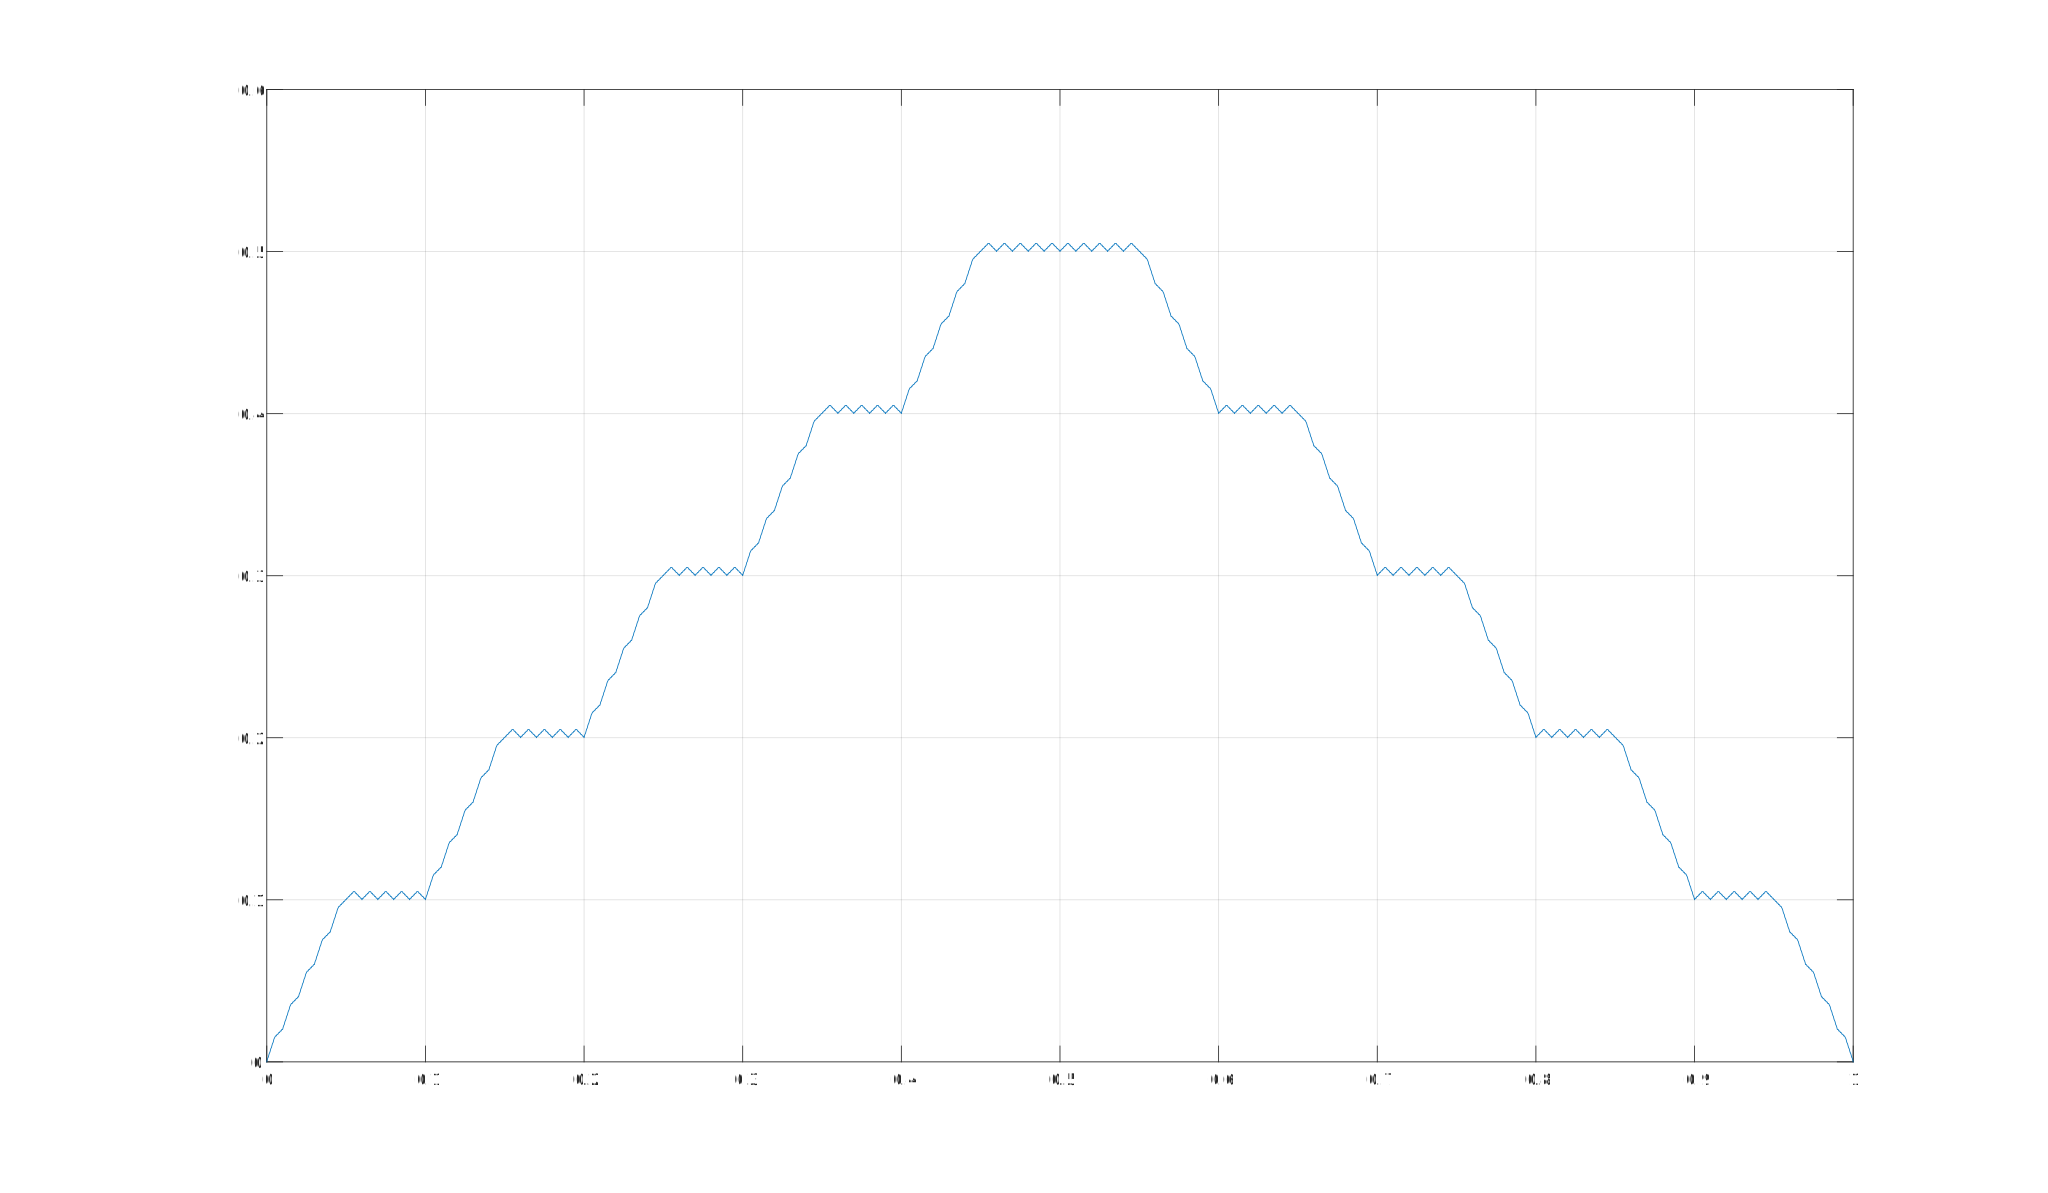
\includegraphics[scale = 0.9]{../figure/奇怪函数}
	\caption{处处连续处处不可导函数}
\end{figure}

\chapter{微分}

\section{微分与导数}

\subsection{微分的定义}

\begin{definition}{可微性}
	称函数$y=f(x)$在$x_0$处可微,如果与$x_0$有关而与$\Delta x$无关的数$A$,使得当$\Delta x\to 0$时,成立
	$$
	\Delta y
	=A\Delta x+o(\Delta x)
	$$
\end{definition}

\begin{note}
	可微必连续,反之不成立,例如$y=|x|$在$0$处不可微。
\end{note}

\subsection{微分与导数}

\begin{definition}{可导性}
	称函数$f(x)$在$x_0$处可导,如果存在极限
	$$
	f'(x_0)=\lim_{x\to x_0}\frac{f(x)-f(x_0)}{x-x_0}
	$$
\end{definition}

\begin{theorem}
	可微$\implies$可导。特别的,对于一元函数,可导与可微等价。
\end{theorem}

\begin{note}
	可导函数的导函数不一定连续,例如
	$$
	f(x)=\begin{cases}
		x^2\sin\frac{1}{x},\qquad & x\ne 0\\
		0,\qquad & x=0
	\end{cases},\qquad 
	f'(x)=\begin{cases}
		2x\sin\frac{1}{x}-\cos\frac{1}{x},\qquad & x\ne 0\\
		0,\qquad & x=0
	\end{cases}
	$$
\end{note}

\subsection{单侧导数}

\begin{definition}{左导数}
	称函数$f(x)$在$x_0$处存在左导数,如果存在极限
	$$
	f'_{-}(x_0)=\lim_{x\to x_0^-}\frac{f(x)-f(x_0)}{x-x_0}
	$$
\end{definition}

\begin{definition}{右导数}
	称函数$f(x)$在$x_0$处存在右导数,如果存在极限
	$$
	f'_{+}(x_0)=\lim_{x\to x_0^+}\frac{f(x)-f(x_0)}{x-x_0}
	$$
\end{definition}

\section{求导法则}

\subsection{导数的四则运算}

\begin{proposition}{导数的四则运算}
	\begin{enumerate}
		\item 和:
		$$
		(f(x)+g(x))'=f'(x)+g'(x)
		$$
		\item 数乘:
		$$
		(\lambda f(x))'=\lambda f'(x)
		$$
		\item 乘法:
		$$
		(f(x)g(x))'=f'(x)g(x)+f(x)g'(x)
		$$
		\item 除法:
		$$
		\left(\frac{f(x)}{g(x)}\right)'
		=\frac{f'(x)g(x)-f(x)g'(x)}{g^2(x)}
		$$
	\end{enumerate}
\end{proposition}

\subsection{反函数求导定理}

\begin{theorem}{反函数求导定理}{反函数求导定理}
	如果函数$y=f(x)$在$(a,b)$上连续、严格单调、可导且$f'(x)\ne 0$,记$\alpha=\min\{ f(a^+),f(b^-) \}$与$\beta=\max\{ f(a^+),f(b^-) \}$,则其反函数$x=f^{-1}(y)$在$(\alpha,\beta)$上可导,且
	$$
	(f^{-1}(y))'=\frac{1}{f'(x)}
	$$
\end{theorem}

\subsection{复合函数求导法则}

\begin{theorem}{复合函数求导法则}{复合函数求导法则}
	如果函数$y=g(x)$在$x_0$处可导,且函数$z=f(y)$在$y_0=g(x_0)$处可导,那么复合函数$f\circ g(x)$在$x_0$处可导,且
	$$
	(f\circ g(x))'
	=f'(g(x_0))g'(x_0)
	$$
	可表示为链式法则
	$$
	\frac{\dd z}{\dd x}
	=\frac{\dd z}{\dd y}\frac{\dd y}{\dd x}
	$$
\end{theorem}

\begin{theorem}{一阶微分的形式不变性}
	复合函数微分公式为
	$$
	\dd (f(g(x)))=f'(g(x))g'(x)\dd x
	$$
	若记$y=g(x)$,那么
	$$
	\dd f(y)=f'(y)\dd y
	$$
\end{theorem}

\section{高阶导数}

\begin{theorem}{Leibniz公式}{Leibniz公式}
	如果函数$f(x)$与$g(x)$均为$n$阶可导函数,那么其积函数$f(x)g(x)$为$n$阶可导函数,且
	$$
	(f(x)g(x))^{(n)}
	=\sum_{k=0}^{n}C_n^k f^{(k)}(x)g^{(n-k)}(x)
	$$
\end{theorem}

\section{导函数的性质}

\begin{theorem}{导数极限定理}
	如果函数$f(x)$在$x_0$邻域内连续,在$x_0$去心邻域内可导,且存在极限$\displaystyle \lim_{x\to x_0} f'(x)$,那么$f(x)$在$x_0$处可导,$f'(x)$在$x_0$处连续。
\end{theorem}

\begin{proof}
	考察$f(x)$在$x_0$处的左导数,由Lagrange中值定理
	$$
	f'_-(x_0)
	=\lim_{x\to x_0^-}\frac{f(x)-f(x_0)}{x-x_0}
	=\lim_{x\to x_0^-}f'(\xi),\qquad x<\xi<x_0
	$$
	由于$f'(x)$在$x_0$处存在左极限,那么
	$$
	\lim_{x\to x_0^-}f'(\xi)=f'(x_0^-)
	$$
	因此
	$$
	f'_-(x_0)=f'(x_0^-)
	$$
	同理可得
	$$
	f'_+(x_0)=f'(x_0^+)
	$$
	由于存在极限$\displaystyle \lim_{x\to x_0} f'(x)$,那么
	$$
	\lim_{x\to x_0} f'(x)=f'(x_0^-)=f'(x_0^+)
	$$
	从而
	$$
	f'_-(x_0)=f'_+(x_0)=\lim_{x\to x_0} f'(x)
	$$
	进而$f(x)$在$x_0$处可导。而
	$$
	f'(x_0)=\lim_{x\to x_0} f'(x)
	$$
	因此$f'(x)$在$x_0$处连续。
\end{proof}

\begin{note}
	如果导数存在左极限,那么存在左导数;如果导数存在右极限,那么存在右导数。
\end{note}

\begin{theorem}{导数无第一类间断点}
	如果函数$f(x)$在$(a,b)$内可导,那么对于任意$x_0\in (a,b)$,或$x_0$为$f'(x)$的连续点,或$x_0$为$f'(x)$的第二类间断点。
\end{theorem}

\begin{proof}
	如果$f'(x)$在$x_0$不存在左右极限之一,那么$x_0$为$f'(x)$的第二类间断点。
	
	如果$f'(x)$在$x_0$处存在左右极限,考察$f(x)$在$x_0$处的左导数,由Lagrange中值定理
	$$
	f'_-(x_0)
	=\lim_{x\to x_0^-}\frac{f(x)-f(x_0)}{x-x_0}
	=\lim_{x\to x_0^-}f'(\xi),\qquad x<\xi<x_0
	$$
	由于$f'(x)$在$x_0$处存在左极限,那么
	$$
	\lim_{x\to x_0^-}f'(\xi)=f'(x_0^-)
	$$
	因此
	$$
	f'_-(x_0)=f'(x_0^-)
	$$
	同理可得
	$$
	f'_+(x_0)=f'(x_0^+)
	$$
	因为$f(x)$在$x_0$处可导,所以
	$$
	f'(x_0)=f'_-(x_0)=f'_+(x_0)
	$$
	从而
	$$
	f'(x_0)=f'(x_0^-)=f'(x_0^+)=\lim_{x\to x_0}f'(x)
	$$
	进而$f'(x)$在$x_0$连续。
\end{proof}

\begin{theorem}{Darboux定理/导数的介值性定理}
	如果函数$f(x)$在$[a,b]$上可导,且$f'(a)<f'(b)$,那么对于任意$f'(a)<\mu<f'(b)$,存在$\xi\in (a,b)$,使得成立$f'(\xi)=\mu$。
\end{theorem}

\begin{proof}
	作辅助函数
	$$
	\varphi(x)=f(x)-\mu x
	$$
	那么$\varphi(x)$在$[a,b]$上可导,且
	$$
	\varphi'(a)=f'(a)-\mu<0,\qquad 
	\varphi'(b)=f'(b)-\mu>0
	$$
	此时存在$\eta_a,\eta_b\in(a,b)$,使得成立
	$$
	g(\eta_a)<g(a),\qquad 
	g(\eta_b)>g(b)
	$$
	于是$g(x)$在端点$a,b$处不取最小值。又因为$g(x)$在$[a,b]$上连续,因此存在$\xi\in (a,b)$,使得$\displaystyle g(\xi)=\min_{a\le x\le b}g(x)$。由Fermat定理,$g'(\xi)=0$,即$f'(\xi)=\mu$。
\end{proof}

\chapter{微分中值定理}

\section{微分中值定理}

\subsection{函数极值与Fermat引理}

\begin{definition}{极大值点}
	称$x_0$为函数$f(x)$的极大值点,如果存在$\delta>0$,使得成立
	$$
	|x-x_0|<\delta\implies
	f(x)\le f(x_0)
	$$
\end{definition}

\begin{definition}{极小值点}
	称$x_0$为函数$f(x)$的极小值点,如果存在$\delta>0$,使得成立
	$$
	|x-x_0|<\delta\implies
	f(x)\ge f(x_0)
	$$
\end{definition}

\begin{theorem}{Fermat引理}{Fermat引理}
	如果$x_0$为函数$f(x)$的极值点,且$f(x)$在$x_0$处可导,那么$f'(x_0)=0$。
\end{theorem}

\begin{proof}
	 不妨$x_0$为$f(x)$的极大值点,因此存在$\delta>0$,使得对于任意$|x-x_0|<\delta$,成立$f(x)\le f(x_0)$。而$f(x)$在$x_0$处可导,因此
	 $$
	 f'(x_0)=\lim_{x\to x_0^+}\frac{f(x)-f(x_0)}{x-x_0}\ge 0,\qquad
	 f'(x_0)=\lim_{x\to x_0^-}\frac{f(x)-f(x_0)}{x-x_0}\le 0
	 $$
	 进而$f'(x_0)=0$。
\end{proof}

\subsection{Rolle定理}

\begin{theorem}{Rolle定理}{Rolle定理}
	如果函数$f(x)$在$[a,b]$上连续,在$(a,b)$上可导,且$f(a)=f(b)$,那么存在$\xi\in (a,b)$,使得成立$f'(\xi)=0$。
\end{theorem}

\subsection{Lagrange定理}

\begin{theorem}{Lagrange定理}
	如果函数$f(x)$在$[a,b]$上连续,在$(a,b)$上可导,那么存在$\xi\in (a,b)$,使得成立
	$$
	f'(\xi)=\frac{f(b)-f(a)}{b-a}
	$$
\end{theorem}

\begin{proof}
	作辅助函数
	$$
	\varphi(x)=f(x)-f(a)-\frac{f(b)-f(a)}{b-a}(x-a)
	$$
	那么
	$$
	\varphi(a)=\varphi(b)=0
	$$
\end{proof}

\begin{corollary}
	如果函数$f(x)$与$g(x)$在$(a,b)$上可导,且$f'(x)\equiv0$,那么$f(x)$在$(a,b)$上为常函数。
\end{corollary}

\begin{theorem}
	如果函数$f(x)$在$(a,b)$上可导,那么
	$$
	f(x)\text{ 在 }(a,b)\text{ 上单调递增}
	\iff 
	\forall x\in (a,b),f'(x)\ge 0
	$$
	特别的,如果$f'(x)$在$(a,b)$中除有限个点外均成立$f'(x)>0$,那么$f(x)$在$(a,b)$上严格单调递增。
\end{theorem}

\subsection{Cauchy定理}

\begin{theorem}{Cauchy定理}{Cauchy定理}
	如果函数$f(x)$与$g(x)$在$[a,b]$上连续,在$(a,b)$上可导,且对于任意$x\in (a,b)$,成立$g'(x)\ne 0$,那么存在$\xi\in (a,b)$,使得成立
	$$
	\frac{f'(\xi)}{g'(\xi)}=\frac{f(b)-f(a)}{g(b)-g(a)}
	$$
\end{theorem}

\subsection{中值定理}

\begin{theorem}{中值定理}
	如果函数$f(x),g(x),h(x)$在$[a,b]$上连续,在$(a,b)$上可导,那么存在$\xi\in (a,b)$,使得成立
	$$
	\begin{vmatrix}
		f(a) & g(a) & h(a)\\
		f(b) & g(b) & h(b)\\
		f'(\xi) & g'(\xi) & h'(\xi)
	\end{vmatrix}=0
	$$
\end{theorem}

\section{L'Hospital法则}

\begin{theorem}{L'Hospital法则}{L'Hospital法则}
	\begin{enumerate}
		\item $\displaystyle\frac{0}{0}$型:设函数$f(x)$与$g(x)$在$x_0$邻域内可导,且在该邻域内$g'(x)\ne 0$,如果
		$$
		\lim_{x\to x_0} f(x)=\lim_{x\to x_0} g(x)=0
		$$
		且极限$\displaystyle\lim_{x\to x_0}\frac{f'(x)}{g'(x)}$存在,那么
		$$
		\lim_{x\to x_0}\frac{f(x)}{g(x)}=\lim_{x\to x_0}\frac{f'(x)}{g'(x)}
		$$
		\item $\displaystyle\frac{*}{\infty}$型:设函数$f(x)$与$g(x)$在$x_0$邻域内可导,且在该邻域内$g'(x)\ne 0$,如果
		$$
		\lim_{x\to x_0} g(x)=\infty
		$$
		且极限$\displaystyle\lim_{x\to x_0}\frac{f'(x)}{g'(x)}$存在,那么
		$$
		\lim_{x\to x_0}\frac{f(x)}{g(x)}=\lim_{x\to x_0}\frac{f'(x)}{g'(x)}
		$$
	\end{enumerate}
\end{theorem}

\begin{theorem}{Stolz公式}
	\begin{enumerate}
		\item $\displaystyle\frac{0}{0}$型:如果$T>0$为常数,且成立如下条件
		\begin{enumerate}
			\item $0<g(x+T)<g(x),\forall x\ge a$
			\item $\displaystyle\lim_{x\to+\infty}f(x)=\lim_{x\to+\infty}g(x)=0$
			\item 存在极限$\displaystyle\lim_{x\to+\infty}\frac{f(x+T)-f(x)}{g(x+T)-g(x)}$
		\end{enumerate}
		那么
		$$
		\lim_{x\to+\infty}\frac{f(x)}{g(x)}=\lim_{x\to+\infty}\frac{f(x+T)-f(x)}{g(x+T)-g(x)}
		$$
		\item $\displaystyle\frac{*}{\infty}$​型:如果$T>0$为常数,且成立如下条件
		\begin{enumerate}
			\item $g(x+T)>g(x),\forall x\ge a$
			\item $\displaystyle\lim_{x\to+\infty}g(x)=+\infty$
			\item $f(x),g(x)$在$[a,\infty)$内闭有界。
			\item 存在极限$\displaystyle\lim_{x\to+\infty}\frac{f(x+T)-f(x)}{g(x+T)-g(x)}$
		\end{enumerate}
		那么
		$$
		\lim_{x\to+\infty}\frac{f(x)}{g(x)}=\lim_{x\to+\infty}\frac{f(x+T)-f(x)}{g(x+T)-g(x)}
		$$
	\end{enumerate}
\end{theorem}

\section{Taylor公式}

\subsection{带Peano余项的Taylor公式}

\begin{theorem}{带Peano余项的Taylor公式}{带Peano余项的Taylor公式}
	如果函数$f(x)$在$x_0$处$n$阶可导,那么存在$x_0$的邻域,使其中任意一点$x$,成立
	$$
	f(x)
	=\sum_{k=0}^{n}\frac{f^{(k)}(x_0)}{k!}(x-x_0)^k+o((x-x_0)^n)
	$$
\end{theorem}

\subsection{带Lagrange余项的Taylor公式}

\begin{theorem}{带Lagrange余项的Taylor公式}{带Lagrange余项的Taylor公式}
	如果函数$f(x)$在$[a,b]$上$n$阶连续可导,在$(a,b)$上$n+1$阶可导,那么对于任意$x,x_0\in [a,b]$,成立
	$$
	f(x)
	=\sum_{k=0}^{n}\frac{f^{(k)}(x_0)}{k!}(x-x_0)^k+
	\frac{f^{(n+1)}(\xi)}{(n+1)!}(x-x_0)^{n+1},\qquad 
	\xi\text{在}x\text{与}x_0\text{之间}
	$$
\end{theorem}

\subsection{初等函数的Taylor公式}

\begin{theorem}{Taylor公式}
	\begin{align*}
		&\mathrm{e}^{x}
		=1+x+\frac{x^2}{2}+\cdots+\frac{x^n}{n!}+o(x^n)
		=\sum_{n=0}^{\infty}{\frac{x^n}{n!}}
		,\quad && x\in\mathbb{R}\\
		&\ln{(1+x)}
		=x-\frac{x^2}{2}+\frac{x^3}{3}-\cdots+\frac{(-1)^{n+1}}{n}x^n+o(x^n)
		=\sum_{n=1}^{\infty}{\frac{(-1)^{n+1}}{n}x^n}
		,\quad && x\in(-1,1]\\
		&\frac{1}{1+x}
		=1-x+x^2-\cdots+(-1)^n x^n+o(x^n)
		=\sum_{n=0}^{\infty}{(-1)^n x^n}
		,\quad && x\in(-1,1)\\
		&\sin{x}
		=x-\frac{x^3}{3!}+\frac{x^5}{5!}-\cdots+\frac{(-1)^n}{(2n+1)!}x^{2n+1}+o(x^{2n+1})
		=\sum_{n=0}^{\infty}{\frac{(-1)^n}{(2n+1)!}x^{2n+1}}
		,\quad && x\in\mathbb{R}\\
		&\cos{x}
		=1-\frac{x^2}{2}+\frac{x^4}{4!}-\cdots+\frac{(-1)^n}{(2n)!}x^{2n}+o(x^{2n})
		=\sum_{n=0}^{\infty}{\frac{(-1)^n}{(2n)!}x^{2n}}
		,\quad && x\in\mathbb{R}\\
		&\arctan{x}
		=x-\frac{x^3}{3}+\frac{x^5}{5}-\cdots+\frac{(-1)^{n+1}}{2n-1}x^{2n-1}+o(x^{2n-1})
		=\sum_{n=1}^{\infty}{\frac{(-1)^{n+1}}{2n-1}x^{2n-1}}
		,\quad && x\in[-1,1]
	\end{align*}
\end{theorem}

\chapter{不定积分}

\section{不定积分的概念与运算法则}

\subsection{不定积分的概念}

\begin{definition}{原函数}
	称函数$F(x)$为$f(x)$的原函数,如果
	$$
	\dd(F(x))=f(x)\dd x
	$$
\end{definition}

\begin{definition}{不定积分}
	称函数$f(x)$的原函数全体为其不定积分,记作
	$$
	\int f(x)\dd x
	$$
\end{definition}

\subsection{不定积分的线性性质}

\begin{theorem}{不定积分的线性性质}
	如果函数$f(x)$与$g(x)$存在原函数,那么对于任意$\lambda\in \R$,成立
	$$
	\int f(x)+g(x)\dd x
	=\int f(x)\dd x+\int g(x)\dd x
	,\qquad
	\int \lambda f(x)\dd x
	=\lambda \int f(x)\dd x
	$$
\end{theorem}

\section{换元积分法与分部积分法}

\subsection{换元积分法}

\begin{theorem}{换元积分法}
	$$
	\int f(x)\dd x
	=\int f(g(t))\dd g(t)
	=\int f(g(t))g'(t)\dd t
	$$
\end{theorem}

\subsection{分部积分法}

\begin{theorem}{分部积分法}
	$$
	\int f(x)g'(x)\dd x
	=f(x)g(x)-\int f'(x)g(x)\dd x
	$$
\end{theorem}

\chapter{定积分}

\section{定积分的概念与可积条件}

\subsection{定积分的概念}

\begin{definition}{Riemann可积性}
	对于$[a,b]$上的有界函数$f(x)$,取$[a,b]$的任意划分
	$$
	\Delta:a=x_0<x_1<\cdots<x_{n-1}<x_n=b
	$$
	记$|\Delta|=\max\limits_{1\le k\le n}|x_{k}-x_{k-1}|$,与$\Delta x_k=|x_k-x_{k-1}|$,其中$1\le k \le n$,对于任意$1\le k\le n$,任取$\xi_k\in[x_{k-1},x_k]$,如果存在极限
	$$
	\lim_{|\Delta|\to 0}\sum_{k=1}^{n}f(\xi_k)\Delta x_k
	$$
	且极限与划分$\Delta$与$\xi_k$的选取无关,那么称$f(x)$在$[a,b]$上Riemann可积,称该极限为$f(x)$在$[a,b]$上的定积分,记作
	$$
	\int_a^b f(x)\dd x
	$$
\end{definition}

\begin{definition}{定积分}
	称$I\in\R$为$[a,b]$上的有界函数$f(x)$的定积分,如果对于任意$\varepsilon>0$,存在$\delta>0$,使得对于任意划分
	$$
	\Delta:a=x_0<x_1<\cdots<x_{n-1}<x_n=b
	$$
	与任意$\xi_k\in[x_{k-1},x_k]$,成立
	$$
	|\Delta|<\delta
	\implies
	\left|\sum_{k=1}^{n}f(\xi_k)\Delta x_k-I\right|<\varepsilon
	$$
	其中$\displaystyle|\Delta|=\max_{1\le k\le n}\Delta x_k$且$\Delta x_k=|x_k-x_{k-1}|$。
\end{definition}

\subsection{Darboux和}

\begin{definition}{Darboux和}
	\begin{enumerate}
		\item 定义$[a,b]$上的有界函数$f(x)$关于划分
		$$
		\Delta:a=x_0<x_1<\cdots<x_{n-1}<x_n=b
		$$
		的Darboux上和为
		$$
		\overline{S}(\Delta)
		=\sum_{k=1}^{n}M_k\Delta x_k
		$$
		其中$\displaystyle M_k=\sup_{x_{k-1}\le x\le x_k}f(x)$且$\Delta x_k=|x_k-x_{k-1}|$。
		\item 定义$[a,b]$上的有界函数$f(x)$关于划分
		$$
		\Delta:a=x_0<x_1<\cdots<x_{n-1}<x_n=b
		$$
		的Darboux下和为
		$$
		\underline{S}(\Delta)
		=\sum_{k=1}^{n}m_k\Delta x_k
		$$
		其中$\displaystyle m_k=\inf_{x_{k-1}\le x\le x_k}f(x)$且$\Delta x_k=|x_k-x_{k-1}|$。
	\end{enumerate}
\end{definition}

\begin{proposition}{Darboux和的性质}
	\begin{enumerate}
		\item 对于任意划分$\Delta$与$\xi_k$的选取,成立
		$$
		\underline{S}(\Delta)
		\le\sum_{k=1}^{n}f(\xi_k)\Delta x_k
		\le\overline{S}(\Delta)
		$$
		\item 对于划分$\Delta_0$的加细$\Delta$,成立
		$$
		\underline{S}(\Delta_0)
		\le\underline{S}(\Delta)
		\le \overline{S}(\Delta)
		\le\overline{S}(\Delta_0)
		$$
		\item 对于任意划分$\Delta_1$与$\Delta_2$,成立
		$$
		\underline{S}(\Delta_1)
		\le \overline{S}(\Delta_2)
		$$
	\end{enumerate}
\end{proposition}

\begin{definition}{上下积分}
	\begin{enumerate}
		\item 定义$[a,b]$上的有界函数$f(x)$的上积分为
		$$
		\overline{\int}_{a}^{b}f(x)\dd x=\inf_{\Delta}\overline{S}(\Delta)=\lim_{|\Delta|\to 0}\overline{S}(\Delta)
		$$
		\item 定义$[a,b]$上的有界函数$f(x)$的下积分为
		$$
		\underline{\int}_{a}^{b}f(x)\dd x=\sup_{\Delta}\underline{S}(\Delta)=\lim_{|\Delta|\to 0}\underline{S}(\Delta)
		$$
	\end{enumerate}
\end{definition}

\begin{theorem}{Darboux定理}{Darboux定理}
	$[a,b]$上的有界函数$f(x)$ Riemann可积的充分必要条件为如下命题。
	\begin{enumerate}
		\item 
		$$
		\overline{\int}_{a}^{b}f(x)\dd x=\underline{\int}_{a}^{b}f(x)\dd x
		$$
		\item 
		$$
		\lim_{|\Delta|\to 0}\sum_{k=1}^{n}\omega_k\Delta x_k=0
		$$
		其中$\omega_k=M_k-m_k$。
		\item 对于任意$\varepsilon>0$,存在划分$\Delta$,使得成立
		$$
		\sum_{k=1}^{n}\omega_k\Delta x_k<\varepsilon
		$$
		\item 对于任意$\varepsilon>0$与$\delta>0$,存在划分$\Delta$,使得成立
		$$
		\sum_{\omega_k\ge\varepsilon}\Delta x_k<\delta
		$$
	\end{enumerate}
\end{theorem}

\begin{theorem}{Riemann可积的方法论}
	\begin{enumerate}
		\item 如果$\displaystyle \sum_{k=1}^{n}\omega_k$有界,那么
		$$
		\sum_{k=1}^{n}\omega_k\Delta x_k\le
		|\Delta|\sum_{k=1}^{n}\omega_k
		$$
		\item 如果$\omega_k<\varepsilon$,那么
		$$
		\sum_{k=1}^{n}\omega_k\Delta x_k\le
		\varepsilon\sum_{k=1}^{n}\Delta x_k
		=\varepsilon(b-a)
		$$
		\item 令
		$$
		\sum \omega_k\Delta x_k
		=\sum' \omega_k\Delta x_k+\sum'' \omega_k\Delta x_k
		$$
		其中
		$$
		\sum' \omega_k\Delta x_k<\frac{\varepsilon}{2(b-a)},\qquad 
		\sum'' \omega_k\Delta x_k<\frac{\varepsilon}{\Omega}
		$$
		这里$\displaystyle \Omega=\sup_{a\le x\le b}f(x)-\inf_{a\le x\le b}f(x)$
	\end{enumerate}
\end{theorem}

\begin{corollary}
	\begin{enumerate}
		\item 闭区间上的连续函数Riemann可积。
		\item 闭区间上的单调函数Riemann可积。
		\item 闭区间上的仅存在有限个间断点的有界函数Riemann可积。
		\item 如果函数$f(x)$在$[a,b]$上仅存在有限个非零点,那么Riemann积分为零。
	\end{enumerate}
\end{corollary}

\section{Riemann可积性}

\begin{theorem}
	$$
	\text{可积}\implies
	\text{绝对可积}\iff
	\text{平方可积}
	$$
\end{theorem}

\begin{theorem}{Riemann可积的Lebesgue准则}
	对于$[a,b]$上的有界函数$f$,成立
	$$
	f\text{ Riemann可积}
	\iff
	f\text{几乎处处连续}
	$$
\end{theorem}

\begin{proof}
	对于充分性,记$f(x)$的不连续点集为
	$$
	D_f=\left\{ x_0\in [a,b]:\lim_{x\to x_0}f(x)\ne f(x_0) \right\}
	=\bigcup_{\delta>0}^{\infty}\left\{ x\in [a,b]:\omega_f(x)>\delta \right\}
	$$
	其中
	$$
	\omega_f(x_0)=\limsup_{x\to x_0}f(x)-\liminf_{x\to x_0}f(x)
	$$
	若要证明$m(D_f)=0$,只需证明对于任意$\delta>0$,$m(D_\delta)=0$,其中
	$$
	D_\delta=\left\{ x\in [a,b]:\omega_f(x)>\delta \right\}
	$$
	
	任取$\varepsilon>0$,由于$f$ Riemann可积,那么存在划分$\Delta$,使得成立
	$$
	\sum_{k=1}^{n}\omega_k\Delta x_k <\delta\varepsilon
	$$
	记
	$$
	S=\{ 1\le k \le n:(x_{k-1},x_k)\cap D_\delta\ne\varnothing \}
	$$
	任取$k\in S$,与$x_0\in (x_{k-1},x_k)\cap D_\delta$,由于
	\begin{align*}
		\omega_k
		& = \sup_{x_{k-1}\le x \le x_k}f(x)-\inf_{x_{k-1}\le x \le x_k}f(x)\\
		& \ge \limsup_{x\to x_0}f(x)-\liminf_{x\to x_0}f(x)\\
		& = \omega_f(x_0)\\
		& >\delta
	\end{align*}
	那么
	$$
	\delta\varepsilon
	>\sum_{k=1}^{n}\omega_k\Delta x_k
	\ge \sum_{k\in S}\omega_k\Delta x_k
	> \delta\sum_{k\in S}\Delta x_k
	\implies
	\sum_{k\in S}\Delta x_k<\varepsilon
	$$
	由于
	$$
	D_\delta\sub \bigcup_{k\in S}(x_{k-1},x_k)\bigcup \bigcup_{k=0}^{n}\{x_k\}
	$$
	那么
	$$
	m(D_\delta)
	\le \sum_{k\in S}\Delta x_k<\varepsilon
	$$
	由$\varepsilon$的任意性,$m(D_\delta)=0$,进而充分性得证!
	
	对于必要性
\end{proof}

\begin{theorem}
	如果有界函数$f(x)$在$[a,b]$上可积,那么$f(x)$在$[a,b]$上存在连续点;换言之,$f(x)$的连续点集在$[a,b]$上稠密。
\end{theorem}

\begin{proof}
	由于$f(x)$在$[a,b]$上可积,那么存在划分$\Delta$,使得成立
	$$
	\sum \omega_k \Delta x_k <\frac{b-a}{2^1}
	$$
	因此存在区间$[x_{k-1},x_{k}]$,使得$f(x)$在$[x_{k-1},x_{k}]$上的振幅
	$$
	\omega_f[x_{k-1},x_{k}] <\frac{1}{2^1}
	$$
	不妨
	$$
	|x_k-x_{k-1}|<\frac{b-a}{2^1},\qquad [x_{k-1},x_{k}] \sub (a,b)
	$$
	记$[x_{k-1},x_{k}]=[a_1,b_1]$。重复上述过程,可得闭区间套$\{[a_n,b_n]\}_{n=1}^{\infty}$,使得对于任意$n\in\N^*$,成立
	$$
	[a_{n+1},b_{n+1}]\sub [a_n,b_n],\qquad
	|a_n-b_n|<\frac{b-a}{2^n},\qquad 
	\omega_f[a_n,b_n] <\frac{1}{2^n}
	$$
	那么由闭区间套定理,存在且存在唯一$\xi\in [a,b]$,使得成立
	$$
	\lim_{n\to\infty} a_n=\lim_{n\to\infty} b_n=\xi
	$$
	容易证明$f(x)$在$\xi$处连续。
\end{proof}

\begin{theorem}
	如果非负函数$f(x)$在$[a,b]$上可积,那么
	$$
	\int_{a}^{b}f(x)\dd x=0
	\iff 
	f\text{ 在连续点上为零 }
	$$
\end{theorem}

\begin{theorem}
	如果有界函数$f(x)$在$[a,b]$上可积,且几乎处处成立$f(x)=0$,那么
	$$
	\int_{a}^{b}f(x)\dd x=0
	$$
\end{theorem}

\section{定积分的基本性质}

\begin{proposition}{定积分的基本性质}
	\begin{enumerate}
		\item 和:如果函数$f(x)$与$g(x)$在$[a,b]$上可积,那么$f(x)+g(x)$在$[a,b]$上可积,且
		$$
		\int_a^b (f(x)+g(x))\dd x
		=\int_a^b f(x)\dd x+\int g(x)\dd x
		$$
		\item 数乘:如果函数$f(x)$在$[a,b]$上可积,那么对于任意$\lambda\in \R$,$\lambda f(x)$在$[a,b]$上可积,且
		$$
		\int_a^b \lambda f(x)\dd x
		=\lambda \int_a^b f(x)\dd x
		$$
		\item 积:如果函数$f(x)$与$g(x)$在$[a,b]$上可积,那么$f(x)g(x)$在$[a,b]$上可积。
		\item 保序性:如果函数$f(x)$在$[a,b]$上可积,且$f(x)\ge 0$,那么
		$$
		\int_a^b f(x)\dd x\ge 0
		$$
		\item 可积$\implies$绝对可积:如果函数$f(x)$在$[a,b]$上可积,那么$|f(x)|$在$[a,b]$上可积,且
		$$
		\left| \int_a^b f(x)\dd x \right|
		\le
		\int_a^b\left|  f(x) \right|\dd x
		$$
		\item 区间可加性:对于$[a,b]$上的函数$f(x)$,以及$a\le c\le b$,成立
		$$
		f(x)\text{ 在 }[a,b]\text{上可积}
		\iff
		f(x)\text{ 在 }[a,c]\text{ 与 }[c,b]\text{上均可积}
		$$
		此时成立
		$$
		\int_a^b f(x)\dd x
		=\int_a^c f(x)\dd x+\int_c^b f(x)\dd x
		$$
	\end{enumerate}
\end{proposition}

\begin{theorem}{积分第一中值定理}
	如果$f(x)$与$g(x)$在$[a,b]$上可积,且$g(x)$不变号,那么存在$\displaystyle \eta\in f([a,b])$,使得成立
	$$
	\int_{a}^{b}f(x)g(x)\dd x
	=\eta\int_{a}^{b}g(x)\dd x
	$$
	特别的,若$f(x)$在$[a,b]$上连续,则存在$\xi\in(a,b)$,使得成立
	$$
	\int_{a}^{b}f(x)g(x)\dd x
	=f(\xi)\int_{a}^{b}g(x)\dd x
	$$
\end{theorem}

\begin{theorem}{积分第二中值定理}
	如果$f(x)$在$[a,b]$上可积,$g(x)$在$[a,b]$上单调,那么存在$\xi\in[a,b]$,使得成立
	$$
	\int_{a}^{b}f(x)g(x)\dd x
	=g(a)\int_{a}^{\xi}f(x)\dd x+g(b)\int_{\xi}^{b}f(x)\dd x
	$$
	特别的,如果$g(x)$在$[a,b]$上单调增加且$g(x)\ge 0$,那么存在$\xi\in[a,b]$,使得成立
	$$
	\int_{a}^{b}f(x)g(x)\dd x
	=g(b)\int_{\xi}^{b}f(x)\dd x
	$$
	如果$g(x)$在$[a,b]$上单调减少且$g(x)\ge 0$,那么存在$\xi\in[a,b]$,使得成立
	$$
	\int_{a}^{b}f(x)g(x)\dd x
	=g(a)\int_{a}^{\xi}f(x)\dd x
	$$
\end{theorem}

\begin{theorem}{Riemann引理}
	\begin{enumerate}
		\item 如果函数$f(x)$在$[a,b]$上可积,$g(x)$以$T$为周期,且在$[0,T]$上可积,那么
		$$
		\lim_{n\to\infty}\int_{a}^{b}f(x)g(nx)\dd x
		=\frac{1}{T}\int_{a}^{b}f(x)\dd x\int_{0}^{T}g(x)\dd x
		$$
		\item 如果函数$f(x)$在$\R$上可积,$g(x)$以$T$为周期,且在$\R$上可积,那么
		$$
		\lim_{n\to\infty}\int_{-\infty}^{+\infty}f(x)g(nx)\dd x
		=\frac{1}{T}\int_{-\infty}^{+\infty}f(x)\dd x\int_{0}^{T}g(x)\dd x
		$$
	\end{enumerate}
\end{theorem}

\begin{theorem}{积分的连续性}
	如果$f(x)$在$[a,b]$的邻域内可积,那么%
	$$
	\lim_{h\to 0}\int_{a}^{b}|f(x+h)-f(x)|\dd x=0
	$$
\end{theorem}

\begin{proposition}
	如果$f(x)$与$g(x)$在$[a,b]$上存在$2n$阶连续导数,且对于任意$0\le k <n$,成立
	$$
	f^{(k)}(a)=f^{(k)}(b)=g^{(k)}(a)=g^{(k)}(b)=0
	$$
	那么
	$$
	\int_{a}^{b}f^{(2n)}(x)g(x)\dd x
	=\int_{a}^{b}f(x)g^{(2n)}(x)\dd x
	$$
\end{proposition}

\section{微积分基本定理}

\subsection{Newton-Leibniz公式}

\begin{theorem}
	如果函数$f(x)$在$[a,b]$上可积,构造函数
	$$
	F(x)=\int_a^x f(t)\dd t
	$$
	那么$F(x)$在$[a,b]$上连续,且若$f(x)$在$[a,b]$上连续,则$F(x)$在$[a,b]$上可导,同时
	$$
	F'(x)=f(x)
	$$
\end{theorem}

\begin{theorem}{微积分基本定理}
	如果函数$f(x)$在$[a,b]$上连续,$F(x)$为$f(x)$在$[a,b]$上的原函数,那么
	$$
	\int_a^b f(x)\dd x=F(b)-F(a)
	$$
\end{theorem}

\subsection{定积分的分部积分法与换元积分法}

\begin{theorem}{分部积分法}
	如果函数$f(x),g(x)$在$[a,b]$连续可导,那么
	$$
	\int_a^b f(x)g'(x)\dd x
	=f(x)g(x)\bigg| _a^b-\int_a^b f'(x)g(x)\dd x
	$$
\end{theorem}

\begin{theorem}{换元积分法}
	如果函数$f(x)$在$[a,b]$连续,$\varphi(t)$在$\alpha$与$\beta$之间连续可导,且像含于$[a,b]$,同时$\varphi(\alpha)=a$与$\varphi(\beta)=b$,那么
	$$
	\int_a^b f(x)\dd x
	=\int_\alpha^\beta f(\varphi(t))\varphi'(t)\dd t
	$$
\end{theorem}

\subsection{定积分的奇偶性与周期性性质}

\begin{theorem}
	如果偶函数$f(x)$在$[-a,a]$上可积,那么
	$$
	\int_{-a}^a f(x)\dd x
	=2\int_{0}^a f(x)\dd x
	$$
	如果奇函数$f(x)$在$[-a,a]$上可积,那么
	$$
	\int_{-a}^a f(x)\dd x
	=0
	$$
\end{theorem}

\begin{theorem}
	如果函数$f(x)$为以$T$为周期的可积函数,那么对于任意$a\in\R$,成立
	$$
	\int_{a}^{a+T} f(x)\dd x
	=\int_{0}^{T} f(x)\dd x
	$$
\end{theorem}

\section{著名不等式}

\begin{theorem}{Cauchy不等式}{Cauchy不等式}
	对于$\{ a_k \}_{k=1}^{n}\sub\R$与$\{ b_k \}_{k=1}^{n}\sub\R$,成立
	$$
	\left(\sum_{k=1}^{n}a_kb_k\right)^2
	\le \left(\sum_{k=1}^{n}a_k^2\right)\left(\sum_{k=1}^{n}b_k^2\right)
	$$
	当且仅当存在$\alpha\in\R$与$\beta\in\R$,使得对于任意$1\le k \le n$,成立$\alpha a_k =\beta b_k$。
\end{theorem}

\begin{theorem}{Schwarz不等式}
	对于$[a,b]$上的可积函数$f(x)$与$g(x)$,成立
	$$
	\left(\int_a^b f(x)g(x)\dd x\right)^2
	\le \left(\int_{a}^{b}f^2(x)\right) \left(\int_{a}^{b}g^2(x)\right)
	$$
	当且仅当存在$\alpha$与$\beta$,使得对于任意$a\le x\le b$,成立$\alpha f(x) =\beta g(x)$。
\end{theorem}

\begin{theorem}{基本不等式}
	对于正实数$x_1,\cdots,x_n$与$\lambda_1,\cdots,\lambda_n$,其中$\lambda_1+\cdots+\lambda_n=1$,定义$r$阶平均函数%
	$$
	M_r(\bs{x},\bs{\lambda})=\left(\sum_{k=1}^{n}\lambda_k x_k^r\right)^{1/r},\qquad r\in\overline{\R}
	$$
	那么$M_r(\bs{x},\bs{\lambda})$关于$r$单调递增,其中
	\small{
	\begin{align*}
		&
		\lim_{r\to -\infty}M_{r}(\bs{x},\bs{\lambda})=\min\{ x_1,\cdots,x_n \} && M_{-1}(\bs{x},\bs{\lambda})=\frac{1}{\frac{\lambda_1}{x_1}+\cdots+\frac{\lambda_n}{x_n}} &&
		\lim_{r\to 0}M_{r}(\bs{x},\bs{\lambda})=x_1^{\lambda_1}\cdots x_n^{\lambda_n}\\
		& M_{1}(\bs{x},\bs{\lambda})=\lambda_1x_1+\cdots+\lambda_nx_n &&
		M_{2}(\bs{x},\bs{\lambda})=\sqrt{\lambda_1x_1^2+\cdots+\lambda_nx_n^2}&&
		\lim_{r\to +\infty}M_{r}(\bs{x},\bs{\lambda})=\max\{ x_1,\cdots,x_n \} 
	\end{align*}}
	且对于任意$r\ne s\in\overline{\R}$,成立%
	$$
	M_{r}(\bs{x},\bs{\lambda})=M_{s}(\bs{x},\bs{\lambda})
	\iff
	x_1=\cdots=x_n
	$$
\end{theorem}

\begin{proof}
	令
	$$
	f(r)
	=\ln M_{r}(\bs{x},\bs{\lambda})
	=\frac{\ln \sum\lambda_k x_k^r}{r}
	$$
	则
	$$
	f'(r)
	=\frac{ r\frac{ \sum\lambda_k x_k^r\ln x_k}{ \sum\lambda_k x_k^r}-\ln\sum\lambda_k x_k^r}{r^2}
	$$
	令
	$$
	g(r)=r\frac{ \sum\lambda_k x_k^r\ln x_k}{ \sum\lambda_k x_k^r}-\ln\sum\lambda_k x_k^r
	$$
	则
	$$
	g'(r)=r\frac{\left( \sum\lambda_k x_k^r \right)\left( \sum\lambda_k x_k^r\ln^2x_k \right)-\left( \sum\lambda_k x_k^r\ln x_k \right)^2}{\left( \sum\lambda_k x_k^r \right)^2}
	$$
	由Cauchy不等式\ref{thm:Cauchy不等式}
	$$
	\left( \sum\lambda_k x_k^r \right)\left( \sum\lambda_k x_k^r\ln^2x_k \right)
	\ge\left( \sum\lambda_k x_k^r\ln x_k \right)^2
	$$
	当且仅当$x_1=\cdots=x_n$时等号成立,则$g'(r)$的符号由$r$决定,从而
	$$
	g(r)\ge g(0)=0
	$$
	因此
	$$
	f'(r)=\frac{g(r)}{r^2}\ge 0
	$$
	进而$f(r)$关于$r$单调递增。
\end{proof}

\chapter{反常积分}

\section{反常积分的概念与计算}

\begin{definition}{反常积分}
	\begin{enumerate}
		\item 对于定义在$[a,+\infty)$上的函数$f(x)$,如果$f(x)$在任意区间$[a,A]$上可积,且存在极限
		$$
		\lim_{A\to+\infty}\int_a^Af(x)\dd x
		$$
		那么称反常积分$\displaystyle \int_a^{+\infty}f(x)\dd x$收敛,其积分值为
		$$
		\int_a^{+\infty}f(x)\dd x=\lim_{A\to+\infty}\int_a^Af(x)\dd x
		$$
		\item 对于定义在$[a,b)$上的函数$f(x)$,如果$\displaystyle \lim_{x\to b^-}f(x)=\infty$,且$f(x)$在任意区间$[a,b-\eta]$上有界可积,同时存在极限
		$$
		\lim_{\eta\to 0^+}\int_a^{b-\eta}f(x)\dd x
		$$
		那么称反常积分$\displaystyle \int_a^bf(x)\dd x$收敛,其积分值为
		$$
		\int_a^bf(x)\dd x=\lim_{\eta\to 0^+}\int_a^{b-\eta}f(x)\dd x
		$$
	\end{enumerate}
\end{definition}

\begin{theorem}{$p$积分的敛散性}
	$$
	\int_1^{+\infty}\frac{1}{x^p}\dd x
	=\begin{cases}
		\frac{1}{p-1},\qquad & p>1\\
		+\infty,\qquad  & p\le 1
	\end{cases},\qquad 
	\int_0^1\frac{1}{x^p}\dd x
	=\begin{cases}
		\frac{1}{1-p},\qquad & p<1\\
		+\infty,\qquad  & p\ge 1
	\end{cases}
	$$
\end{theorem}

\section{反常积分的收敛判别法}

\subsection{Cauchy收敛原理}

\begin{theorem}{Cauchy收敛原理}
	\begin{enumerate}
		\item 反常积分$\displaystyle \int_a^{+\infty}f(x)\dd x$收敛的充分必要条件为:对于任意$\varepsilon>0$,存在$A\ge a$,使得对于任意$A_1,A_2\ge A$,成立
		$$
		\left| \int_{A_1}^{A_2}f(x)\dd x \right|<\varepsilon
		$$
		\item 反常积分$\displaystyle \int_a^{b}f(x)\dd x$收敛的充分必要条件为:对于任意$\varepsilon>0$,存在$\delta>0$,使得对于任意$\eta_1,\eta_2\in (0,\delta)$,成立
		$$
		\left| \int_{\eta_1}^{\eta_2}f(x)\dd x \right|<\varepsilon
		$$
	\end{enumerate}
\end{theorem}

\subsection{比较判别法}

\begin{theorem}{比较判别法}
	如果在$[a,+\infty)$上成立$0\le f(x) \le \varphi(x)$,那么
	\begin{enumerate}
		\item 若$\displaystyle \int_a^{+\infty}\varphi(x)\dd x$收敛,则$\displaystyle \int_a^{+\infty}f(x)\dd x$收敛。
		\item 若$\displaystyle \int_a^{+\infty}f(x)\dd x$发散,则$\displaystyle \int_a^{+\infty}\varphi(x)\dd x$发散。
	\end{enumerate}
\end{theorem}

\begin{theorem}{比较判别法的极限形式}
	如果在$[a,+\infty)$上成立$f(x)\ge 0$,且
	$$
	\lim_{x\to+\infty}\frac{f(x)}{\varphi(x)}=l
	$$
	那么
	\begin{enumerate}
		\item 若$0<l<+\infty$,则$\displaystyle \int_a^{+\infty}\varphi(x)\dd x$与$\displaystyle \int_a^{+\infty}f(x)\dd x$敛散性相同。
		\item 若$l=0$,则$\displaystyle \int_a^{+\infty}\varphi(x)\dd x$收敛时$\displaystyle \int_a^{+\infty}f(x)\dd x$收敛。
		\item 若$l=+\infty$,则$\displaystyle \int_a^{+\infty}\varphi(x)\dd x$发散时$\displaystyle \int_a^{+\infty}f(x)\dd x$发散。
	\end{enumerate}
\end{theorem}

\subsection{Cauchy判别法}

\begin{theorem}{Cauchy判别法}
	\begin{enumerate}
		\item 如果在$[a,+\infty)$上成立$f(x)\ge 0$,那么
		\begin{enumerate}
			\item 若$\displaystyle f(x)\le\frac{1}{x^p}$且$p>1$,则$\displaystyle \int_a^{+\infty}f(x)\dd x$收敛。
			\item 若$\displaystyle f(x)\ge\frac{1}{x^p}$且$p\le 1$,则$\displaystyle \int_a^{+\infty}\varphi(x)\dd x$发散。
		\end{enumerate}
		\item 如果在$[a,b)$上成立$f(x)\ge 0$,那么
		\begin{enumerate}
			\item 若$\displaystyle f(x)\le\frac{1}{(b-x)^p}$且$p<1$,则$\displaystyle \int_a^{b}f(x)\dd x$收敛。
			\item 若$\displaystyle f(x)\ge\frac{1}{(b-x)^p}$且$p\ge 1$,则$\displaystyle \int_a^{+\infty}\varphi(x)\dd x$发散。
		\end{enumerate}
	\end{enumerate}
\end{theorem}

\begin{theorem}{Cauchy判别法的极限形式}
	\begin{enumerate}
		\item 如果在$[a,+\infty)$上成立$f(x)\ge 0$,且
		$$
		\lim_{x\to+\infty}x^pf(x)=l
		$$
		那么
		\begin{enumerate}
			\item 若$0\le l <+\infty$且$p>1$,则$\displaystyle \int_a^{+\infty}f(x)\dd x$收敛。
			\item 若$0<l \le+\infty$且$p\le 1$,则$\displaystyle \int_a^{+\infty}f(x)\dd x$发散。
		\end{enumerate}
		\item 如果在$[a,b)$上成立$f(x)\ge 0$,且
		$$
		\lim_{x\to+\infty}(b-x)^pf(x)=l
		$$
		那么
		\begin{enumerate}
			\item 若$0\le l <+\infty$且$p<1$,则$\displaystyle \int_a^{+\infty}f(x)\dd x$收敛。
			\item 若$0<l \le+\infty$且$p\ge 1$,则$\displaystyle \int_a^{+\infty}f(x)\dd x$发散。
		\end{enumerate}
	\end{enumerate}
\end{theorem}

\subsection{Abel判别法与Dirichlet判别法}

\begin{theorem}{Abel判别法}
	\begin{enumerate}
		\item 如果$f(x)$在$[a,+\infty)$上单调有界,且$\displaystyle \int_a^{+\infty}g(x)\dd x$收敛,那么$\displaystyle \int_a^{+\infty}f(x)g(x)\dd x$收敛。
		\item 如果$f(x)$在$[a,b)$上单调有界,且$\displaystyle \int_a^{b}g(x)\dd x$收敛,那么$\displaystyle \int_a^bf(x)g(x)\dd x$收敛。
	\end{enumerate}
\end{theorem}

\begin{theorem}{Dirichlet判别法}
	\begin{enumerate}
		\item 如果$\displaystyle F(A)=\int_a^{A}f(x)\dd x$在$[a,+\infty)$上有界,且$g(x)$在$[a,+\infty)$上单调,同时$\displaystyle \lim_{x\to +\infty}g(x)=0$,那么$\displaystyle \int_a^{+\infty}f(x)g(x)\dd x$收敛。
		\item 如果$\displaystyle F(\eta)=\int_a^{b-\eta}f(x)\dd x$在$(0,b-a]$上有界,且$g(x)$在$[a,b)$上单调,同时$\displaystyle \lim_{x\to b^-}g(x)=0$,那么$\displaystyle \int_a^{b}f(x)g(x)\dd x$收敛。
	\end{enumerate}
\end{theorem}

\section{反常积分的敛散性}

\begin{theorem}
	对于反常积分
	$$
	I=\int_{0}^{+\infty}x^\alpha\sin x^\beta\dd x
	$$
	\begin{enumerate}
		\item 若$\beta\ne0$且$-1<\frac{\alpha+1}{\beta}<0$,则绝对收敛。
		\item 若$\beta\ne0$且$0\le \frac{\alpha+1}{\beta}<1$,则条件收敛。
		\item 若为其他情况,则发散。
	\end{enumerate}
\end{theorem}

\begin{proof}
	如果$\beta=0$,那么
	$$
	I=\sin 1\int_{0}^{1}x^\alpha\dd x+\sin 1\int_{1}^{+\infty}x^\alpha\dd x
	$$
	此时对于任意$\alpha\in\R$,原积分发散。
	
	如果$\beta\ne 0$,那么令
	$$
	t=x^\beta,\qquad 
	\lambda=\frac{\alpha+1}{\beta}-1
	$$
	成立
	$$
	I = \frac{1}{|\beta|}\int_{0}^{+\infty}t^{\lambda}\sin t\dd t
	= \frac{1}{|\beta|}\int_{0}^{1}t^{\lambda}\sin t\dd t+\frac{1}{|\beta|}\int_{1}^{+\infty}t^{\lambda}\sin t\dd t
	= \frac{1}{|\beta|}(I_1+I_2)
	$$
	
	考察$I_1$,由于
	$$
	\lim_{t\to 0^+}\frac{t^\lambda \sin t}{t^{\lambda+1}}=1
	$$
	因此$I_1$与$\displaystyle \int_{0}^{1}t^{\lambda+1}\dd t$同具敛散性。又因为
	$$
	\int_{0}^{1}t^{\lambda+1}\dd t=\begin{cases}
		\frac{1}{\lambda+2},\qquad & \lambda >-2\\
		+\infty,\qquad & \lambda \le -2
	\end{cases}
	$$
	从而当且仅当$\lambda >-2$时积分$I_1$收敛。又由于被积函数非负,收敛即为绝对收敛。
	
	考察$I_2$,此时仅需考虑$\lambda >-2$。
	
	i) 当$-2<\lambda <-1$时,因为
	$$
	|t^{\lambda}\sin t|\le t^{\lambda},\qquad 
	\int_{1}^{+\infty}t^{\lambda}\dd t=-\frac{1}{\lambda+1}
	$$
	所以$I_2$绝对收敛。
	
	ii) 当$-1\le \lambda <0$时,因为$t^\lambda$单调递减趋于$0$,且对于任意$A\ge 1$
	$$
	\left| \int_{1}^{A}\sin t\dd t \right|=|\cos 1 - \cos A|\le 2
	$$
	所以由Dirichlet判别法,$I_2$收敛。
	
	由于
	$$
	|t^{\lambda}\sin t|
	\ge t^{\lambda}\sin^2 t
	= \frac{1}{2}(t^{\lambda}-t^{\lambda}\cos 2t)
	$$
	容易知道反常积分$\displaystyle \int_{1}^{+\infty}t^{\lambda}\dd t$发散。考察积分
	$$
	I_2'=\int_{1}^{+\infty}t^{\lambda}\cos 2t\dd t
	$$
	因为$t^\lambda$单调递减趋于$0$,且对于任意$A\ge 1$
	$$
	\left| \int_{1}^{A}\cos 2t+\dd t \right|=\frac{1}{2}|\sin A - \sin 1|\le 1
	$$
	所以由Dirichlet判别法,$I_2'$收敛,从而反常积分$\displaystyle \int_{1}^{+\infty}|t^{\lambda}\sin t|\dd t$发散,进而$I_2$条件收敛。
	
	iii) 当$\mu\ge 0$时,由于对于任意$n\in\N^*$,成立
	$$
	\left| \int_{2n\pi}^{(2n+1)\pi}t^\lambda\sin t\dd t \right|
	\ge \int_{2n\pi}^{(2n+1)\pi}|t^\lambda|\sin t\dd t
	\ge \int_{2n\pi}^{(2n+1)\pi}\sin t\dd t
	= 2
	$$
	那么由Cauchy收敛准则,$I_2$发散。
	
	综上所述,原积分当$\beta\ne0$且$-1<\frac{\alpha+1}{\beta}<0$时,绝对收敛;当$\beta\ne0$且$0\le \frac{\alpha+1}{\beta}<1$时,条件收敛;其他情况发散。
\end{proof}

\begin{theorem}{绝对可积$\implies$可积}
	如果函数$|f(x)|$在$[a,+\infty)$上可积,那么$f(x)$在$[a,+\infty)$上可积。
\end{theorem}

\begin{theorem}
	如果反常积分$\displaystyle \int_a^{+\infty}f(x)\dd x$收敛,且$f(x)$在$[a,+\infty)$上一致连续,那么
	$$
	\lim_{x\to +\infty}f(x)=0
	$$
\end{theorem}

\begin{theorem}
	如果反常积分$\displaystyle \int_a^{+\infty}f(x)\dd x$收敛,且存在极限$\displaystyle \lim_{x\to +\infty}f(x)$,那么
	$$
	\lim_{x\to +\infty}f(x)=0
	$$
\end{theorem}

\begin{theorem}
	如果反常积分$\displaystyle \int_a^{+\infty}f(x)\dd x$收敛,且$f(x)$在$[a,+\infty)$上单调递减,那么
	$$
	\lim_{x\to +\infty}xf(x)=0
	$$
\end{theorem}

\begin{theorem}
	如果反常积分$\displaystyle \int_a^{+\infty}f(x)\dd x$收敛,且$xf(x)$在$[a,+\infty)$上单调递减,那么
	$$
	\lim_{x\to +\infty}xf(x)\ln x-=0
	$$
\end{theorem}

\chapter{数项级数}

\section{数项级数}

\subsection{数项级数的收敛性}

\begin{definition}{数项级数}
	称数项级数$\displaystyle \sum_{n=1}^{\infty}x_n$收敛于$S$,如果部分和数列$\{ S_n \}_{n=1}^{\infty}$收敛于$S$,其中$S_n=\displaystyle \sum_{k=1}^{n}x_k$。
\end{definition}

\begin{definition}{等比级数}
	$$
	\sum_{n=0}^{\infty}q^n=\begin{cases}
		\frac{1}{1-q},\qquad & |q|<1\\
		+\infty,\qquad & q\ge 1
	\end{cases}
	$$
\end{definition}

\subsection{数项级数的基本性质}

\begin{theorem}{级数收敛的必要条件}
	如果数项级数$\displaystyle \sum_{n=1}^{\infty}x_n$收敛,那么
	$$
	\lim_{n\to\infty}x_n=0
	$$
\end{theorem}

\begin{theorem}{数项级数的加法结合律}
	如果数项级数$\displaystyle \sum_{n=1}^{\infty}x_n$收敛,那么其求和式中任意添加括号后所得级数仍收敛,且和不变。
\end{theorem}

\begin{theorem}{$p$级数}
	$$
	\sum_{n=1}^{\infty}\frac{1}{n^p}\begin{cases}
		<\infty,\qquad & p>1\\
		=\infty,\qquad & p\le 1
	\end{cases}
	$$
\end{theorem}

\begin{definition}{Riemann $\zeta$函数}
	$$
	\zeta(s)=\sum_{n=1}^{\infty}\frac{1}{n^s}
	$$
	\begin{enumerate}
		\item $\zeta(2)=\pi^2/6$
		\item $\zeta(4)=\pi^4/90$
		\item $\zeta(6)=\pi^6/945$
		\item $\zeta(8)=\pi^8/9450$
		\item $\zeta(10)=\pi^{10}/93555$
	\end{enumerate}
\end{definition}

\section{上极限与下极限}

\begin{definition}{数列的上极限}
	对于有界数列$\{x_n\}_{n=1}^{\infty}$,定义其上极限如下。
	\begin{enumerate}
		\item 
		$$
		\varlimsup_{n\to\infty}{x_n}=\lim_{n\to\infty}{\sup_{m\ge n}{x_m}}=\inf_{n\ge 1}{\sup_{m\ge n}{x_m}}
		$$
		\item 若$\displaystyle\varlimsup_{n\to\infty}{x_n}=a$,则成立
		\begin{itemize}
			\item 对于任意$\varepsilon>0$,存在$N\in\N^*$,使得对于任意$n\ge N$,成立$x_n< a+\varepsilon$。
			\item 对于任意$\varepsilon>0$与$N\in\N^*$,存在$n\ge N$,使得成立$x_n> a-\varepsilon$。
		\end{itemize}
	\end{enumerate}
	
	对于无上界数列$\{x_n\}_{n=1}^{\infty}$,定义$\displaystyle\varlimsup_{n\to\infty}{x_n}=+\infty$;特别的,如果$\displaystyle\lim_{n\to\infty}{x_n}=+\infty$,定义$\displaystyle\varlimsup_{n\to\infty}{x_n}=\varliminf_{n\to\infty}{x_n}=+\infty$。
\end{definition}

\begin{definition}{数列的下极限}
	对于有界数列$\{x_n\}_{n=1}^{\infty}$,定义其下极限如下。
	\begin{enumerate}
		\item 
		$$
		\varliminf_{n\to\infty}{x_n}=\lim_{n\to\infty}{\inf_{m\ge n}{x_m}}=\sup_{n\ge 1}{\inf_{m\ge n}{x_m}}
		$$
		\item 若$\displaystyle\varliminf_{n\to\infty}{x_n}=a$,则成立
		\begin{itemize}
			\item 对于任意$\varepsilon>0$,存在$N\in\N^*$,使得对于任意$n\ge N$,成立$x_n> a-\varepsilon$。
			\item 对于任意$\varepsilon>0$与$N\in\N^*$,存在$n\ge N$,使得成立$x_n< a+\varepsilon$。
		\end{itemize}
	\end{enumerate}
	
	对于无下界数列$\{x_n\}_{n=1}^{\infty}$,定义$\displaystyle\varliminf_{n\to\infty}{x_n}=-\infty$;特别的,如果$\displaystyle\lim_{n\to\infty}{x_n}=-\infty$,定义$\displaystyle\varlimsup_{n\to\infty}{x_n}=\varliminf_{n\to\infty}{x_n}=-\infty$。
\end{definition}

\begin{proposition}{数列的上下极限性质}
	对于数列$\{x_n\}_{n=1}^{\infty}$与$\{y_n\}_{n=1}^{\infty}$,成立如下命题。
	\begin{enumerate}
		\item 
		$$
		\varliminf_{n\to\infty}{x_n}+\varliminf_{n\to\infty}{y_n}
		\le \varliminf_{n\to\infty}{(x_n+y_n)}
		\le \varliminf_{n\to\infty}{x_n}+\varlimsup_{n\to\infty}{y_n}
		\le \varlimsup_{n\to\infty}{(x_n+y_n)}
		\le \varlimsup_{n\to\infty}{x_n}+\varlimsup_{n\to\infty}{y_n}
		$$
		其中若$\{x_n\}_{n=1}^{\infty}$或$\{y_n\}_{n=1}^{\infty}$收敛,则等号成立。
		\item 若$\{x_n\}_{n=1}^{\infty}$与$\{y_n\}_{n=1}^{\infty}$非负,则
		$$
		\varliminf_{n\to\infty}{x_n}\cdot\varliminf_{n\to\infty}{y_n}
		\le \varliminf_{n\to\infty}{x_ny_n}
		\le \varliminf_{n\to\infty}{x_n}\cdot\varlimsup_{n\to\infty}{y_n}
		\le \varlimsup_{n\to\infty}{x_ny_n}
		\le \varlimsup_{n\to\infty}{x_n}\cdot\varlimsup_{n\to\infty}{y_n}
		$$
		其中若$\{x_n\}_{n=1}^{\infty}$或$\{y_n\}_{n=1}^{\infty}$收敛,则等号成立。
		\item 若$\{x_n\}_{n=1}^{\infty}$非负,则
		$$
		\varliminf_{n\to\infty}\frac{x_{n+1}}{x_n}
		\le \varliminf_{n\to\infty}\sqrt[n]{x_n}
		\le \varlimsup_{n\to\infty}\sqrt[n]{x_n}
		\le \varlimsup_{n\to\infty}\frac{x_{n+1}}{x_n}
		$$
		\item 存在收敛子列$\{x_{n_k}\}_{k=1}^{\infty}$,使得成立
		$$
		\lim_{k\to\infty}x_{n_k}=\varlimsup_{n\to\infty}{x_n}
		$$
		\item 存在收敛子列$\{x_{n_k}\}_{k=1}^{\infty}$,使得成立
		$$
		\lim_{k\to\infty}x_{n_k}=\varliminf_{n\to\infty}{x_n}
		$$
		\item 对于任意收敛子列$\{x_{n_k}\}_{k=1}^{\infty}$,成立
		$$
		\varliminf_{n\to\infty}{x_n}\le
		\lim_{k\to\infty}x_{n_k}
		\le\varlimsup_{n\to\infty}{x_n}
		$$
		\item 对于任意子列$\{x_{n_k}\}_{k=1}^{\infty}$,成立
		$$
		\varlimsup_{k\to\infty}x_{n_k}\le\varlimsup_{n\to\infty}x_{n},
		\qquad
		\varliminf_{k\to\infty}x_{n_k}\ge\varliminf_{n\to\infty}x_{n}
		$$
	\end{enumerate}
\end{proposition}

\section{正项级数}

\subsection{正项级数}

\begin{definition}{正项级数}
	称数项级数$\displaystyle \sum_{n=1}^{\infty}x_n$为正项级数,如果对于任意$n\in\N^*$,成立$x_n\ge 0$。
\end{definition}

\begin{theorem}{正项级数的收敛原理}
	正项级数收敛的充分必要条件为其部分和数列存在上界。
\end{theorem}

\subsection{比较判别法}

\begin{definition}{比较判别法}
	对于正项级数$\displaystyle \sum_{n=1}^{\infty}x_n$与$\displaystyle \sum_{n=1}^{\infty}y_n$,如果对于任意$n\in\N^*$,成立
	$$
	x_n\le y_n
	$$
	那么
	\begin{enumerate}
		\item 若$\displaystyle \sum_{n=1}^{\infty}y_n$收敛,则$\displaystyle \sum_{n=1}^{\infty}x_n$收敛。
		\item 若$\displaystyle \sum_{n=1}^{\infty}x_n$发散,则$\displaystyle \sum_{n=1}^{\infty}y_n$发散。
	\end{enumerate}
\end{definition}

\begin{definition}{比较判别法的极限形式}
	对于正项级数$\displaystyle \sum_{n=1}^{\infty}x_n$与$\displaystyle \sum_{n=1}^{\infty}y_n$,如果
	$$
	\lim_{n\to\infty}\frac{x_n}{y_n}=l
	$$
	那么
	\begin{enumerate}
		\item $0<l<+\infty$,则$\displaystyle \sum_{n=1}^{\infty}y_n$与$\displaystyle \sum_{n=1}^{\infty}x_n$敛散性相同。
		\item 若$l=0$,则$\displaystyle \sum_{n=1}^{\infty}y_n$收敛时,$\displaystyle \sum_{n=1}^{\infty}x_n$收敛。
		\item 若$l=+\infty$,则$\displaystyle \sum_{n=1}^{\infty}y_n$发散时,$\displaystyle \sum_{n=1}^{\infty}x_n$发散。
	\end{enumerate}
\end{definition}

\subsection{Cauchy判别法}

\begin{theorem}{Cauchy判别法}
	对于正项级数$\displaystyle \sum_{n=1}^{\infty}x_n$,若记
	$$
	r=\varlimsup_{n\to\infty} \sqrt[n]{x_n}
	$$
	则
	\begin{enumerate}
		\item $r<1$:级数$\displaystyle \sum_{n=1}^{\infty}x_n$收敛。
		\item $r>1$:级数$\displaystyle \sum_{n=1}^{\infty}x_n$发散。
	\end{enumerate}
\end{theorem}

\subsection{d'Alembert判别法}

\begin{theorem}{d'Alembert判别法}
	对于正项级数$\displaystyle \sum_{n=1}^{\infty}x_n$,若记
	$$
	\overline{r}=\varlimsup_{n\to\infty} \frac{x_{n+1}}{x_n},\qquad 
	\underline{r}=\varliminf_{n\to\infty} \frac{x_{n+1}}{x_n}
	$$
	则
	\begin{enumerate}
		\item $\overline{r}<1$:级数$\displaystyle \sum_{n=1}^{\infty}x_n$收敛。
		\item $\underline{r}>1$:级数$\displaystyle \sum_{n=1}^{\infty}x_n$发散。
	\end{enumerate}
\end{theorem}

\subsection{Rabbe判别法}

\begin{theorem}{Rabbe判别法}
	对于级数$\displaystyle \sum_{n=1}^{\infty}x_n$,若记
	$$
	r=\lim_{n\to\infty} n\left(\left|\frac{x_n}{x_{n+1}}\right|-1\right)
	$$
	则
	\begin{enumerate}
		\item $r>1$:级数$\displaystyle \sum_{n=1}^{\infty}x_n$绝对收敛。
		\item $r<1$:级数$\displaystyle \sum_{n=1}^{\infty}x_n$发散。
	\end{enumerate}
\end{theorem}

\subsection{积分判别法}

\begin{theorem}{积分判别法}
	对于定义在$[a,+\infty)$上的非负函数$f(x)$,如果$f(x)$在任意区间$[a,A]$上可积,取单调递增趋于$+\infty$的数列$\{a_n\}_{n=1}^{\infty}$,令
	$$
	x_n=\int_{a_n}^{a_{n+1}}f(x)\dd x
	$$
	那么反常积分$\displaystyle \int_a^{+\infty}f(x)\dd x$与正项级数$\displaystyle \sum_{n=1}^{\infty}x_n$同时收敛或同时发散于$+\infty$,且
	$$
	\int_a^{+\infty}f(x)\dd x
	=\sum_{n=1}^{\infty}x_n
	$$
\end{theorem}

\begin{theorem}{Cauchy积分判别法}
	对于定义在$[0,+\infty)$上的非负单调递减函数$f(x)$,成立
	$$
	\text{数项级数}\sum_{n=1}^{\infty}f(n)\text{与}
	\text{反常积分}\int_0^{+\infty}f(x)\dd x\text{的敛散性相同}
	$$
\end{theorem}

\subsection{Cauchy凝聚判别法}

\begin{theorem}{Cauchy凝聚判别法}
	对于单调递减的正项数列$\{ x_n \}_{n=1}^{\infty}$,成立%
	$$
	\text{级数}\sum_{n=1}^{\infty}x_n\text{与}
	\text{级数}\sum_{n=1}^{\infty}2^nx_{2^n}\text{的敛散性相同}
	$$
\end{theorem}

\section{任意项级数}

\subsection{任意项级数}

\begin{theorem}{Cauchy收敛原理}
	级数$\dis \sum_{n=1}^{\infty}x_n$收敛的充分必要条件是:对于任意$\varepsilon>0$,存在$N\in\N^*$,使得对于任意$m\ge n\ge N$成立
	$$
	\left| \sum_{k=n}^{m}x_k \right|<\varepsilon
	$$
\end{theorem}

\begin{corollary}{级数收敛的必要原理}
	如果级数$\dis \sum_{n=1}^{\infty}x_n$收敛,那么$\dis \lim_{n\to\infty}x_n=0$。
\end{corollary}

\subsection{Leibniz级数}

\begin{theorem}{Leibniz判别法}
	如果正项级数$\{x_n\}_{n=1}^{\infty}$单调递减趋于$0$,那么交错级数$\dis \sum_{n=1}^{\infty}(-1)^{n+1}x_n$收敛。
\end{theorem}

\begin{corollary}
	如果Leibniz级数$\dis \sum_{n=1}^{\infty}(-1)^{n+1}x_n$收敛,那么对于$n\in\N^*$,成立
	$$
	0\le\sum_{n=1}^{\infty}(-1)^{n+1}x_n\le x_1,\qquad 
	\left| \sum_{k=n}^{\infty}(-1)^{k+1}x_k \right|\le x_n
	$$
\end{corollary}

\subsection{Abel判别法与Dirichlet判别法}

\begin{theorem}{Abel变换}
	对于数列$\{a_n\}_{n=1}^{\infty}$与$\{b_n\}_{n=1}^{\infty}$,记$\Delta a_n=a_{n+1}-a_n$,$\dis B_n=\sum_{k=1}^{n}b_k$,那么
	$$
	\sum_{k=1}^{n}a_kb_k
	=a_nB_n-\sum_{k=1}^{n-1}\Delta a_k B_k
	$$
\end{theorem}

\begin{theorem}{Abel判别法}
	如果数列$\{a_n\}_{n=1}^{\infty}$单调且有界,同时级数$\dis\sum_{n=1}^{\infty}b_n$收敛,那么级数$\dis\sum_{n=1}^{\infty}a_nb_n$收敛。
\end{theorem}

\begin{theorem}{Dirichlet判别法}
	如果数列$\{a_n\}_{n=1}^{\infty}$单调趋于$0$,同时数列$\dis\left\{\sum_{k=1}^{n}b_k\right\}_{n=1}^{\infty}$有界,那么级数$\dis\sum_{n=1}^{\infty}a_nb_n$收敛。
\end{theorem}

\subsection{绝对收敛与条件收敛}

\begin{definition}{绝对收敛}
	称级数$\dis \sum_{n=1}^{\infty}x_n$绝对收敛,如果级数$\dis \sum_{n=1}^{\infty}|x_n|$收敛。
\end{definition}

\begin{definition}{条件收敛}
	称级数$\dis \sum_{n=1}^{\infty}x_n$条件收敛,如果级数$\dis \sum_{n=1}^{\infty}x_n$收敛且级数$\dis \sum_{n=1}^{\infty}|x_n|$发散。
\end{definition}

\begin{theorem}
	如果级数绝对收敛,那么其任意更序级数均收敛,且收敛值相等。
\end{theorem}

\begin{theorem}{Riemann重排定理}
	如果级数$\dis \sum_{n=1}^{\infty}x_n$条件收敛,那么对于任意$a\in\overline{\R}$,存在更序级数$\dis \sum_{n=1}^{\infty}x_n'$,使得成立
	$$
	\sum_{n=1}^{\infty}x_n'=a
	$$
\end{theorem}

\subsection{级数的乘法}

\begin{definition}{Cauchy乘积}
	定义级数$\dis \sum_{n=1}^{\infty}a_n$与$\dis \sum_{n=1}^{\infty}b_n$的Cauchy乘积为
	$$
	\sum_{n=1}^{\infty}\sum_{i+j=n}a_ib_j
	$$
\end{definition}

\begin{theorem}
	如果级数$\dis \sum_{n=1}^{\infty}a_n$与$\dis \sum_{n=1}^{\infty}b_n$均绝对收敛,那么其任意乘积亦绝对收敛,且和为$\dis\left(\sum_{n=1}^{\infty}a_n\right)\left(\sum_{n=1}^{\infty}b_n\right)$。
\end{theorem}

\subsection{级数问题的反例}

\begin{theorem}
	如果级数$\dis \sum_{n=1}^{\infty}x_n$收敛,且$x_n>0$,同时$x_n$单调递减,那么$\dis \lim_{n\to\infty}nx_n=0$。
\end{theorem}

\begin{example}
	去掉“$x_n$单调递减”条件,结论不成立。例如,记
	$$
	x_n=\begin{cases}
		\frac{1}{n},\qquad & n\text{为平方数}\\
		\frac{1}{n^2},\qquad & \text{其他}
	\end{cases}
	$$
\end{example}

\begin{theorem}{Leibniz级数}
	对于单调递减的正项数列$\{x_n\}_{n=1}^{\infty}$,如果$\dis\lim_{n\to\infty} x_n=0$,那么交错级数$\dis \sum_{n=1}^{\infty}(-1)^nx_n$发散。
\end{theorem}

\begin{example}
	去掉“$x_n$单调递减”条件,结论不成立。例如,记
	$$
	x_n=\begin{cases}
		\frac{1}{n^2},\qquad & n\text{为奇数}\\
		\frac{1}{n^2},\qquad & n\text{为偶数}
	\end{cases}
	$$
\end{example}

\section{无穷乘积}

\begin{definition}{无穷乘积收敛}
	称无穷乘积$\dis \prod_{n=1}^{\infty}p_n$收敛,如果
	$$
	\lim_{n\to\infty}\prod_{k=1}^{n}p_k=a\in\R\setminus\{0\}
	$$
\end{definition}

\begin{theorem}
	如果无穷乘积$\dis \prod_{n=1}^{\infty}p_n$收敛,那么
	$$
	\lim_{n\to\infty}p_n=1,\qquad 
	\lim_{n\to\infty}\prod_{k=n}^{\infty}p_k=1
	$$
\end{theorem}

\begin{theorem}
	$$
	\text{无穷乘积 }\prod_{n=1}^{\infty}p_n\text{ 收敛}
	\iff
	\text{级数 }\sum_{n=1}^{\infty}\ln p_n\text{ 收敛}
	$$
\end{theorem}

\begin{definition}{绝对收敛}
	称无穷乘积$\dis \prod_{n=1}^{\infty}p_n$绝对收敛,如果级数$\dis \sum_{n=1}^{\infty}\ln p_n$绝对收敛。
\end{definition}

\chapter{函数项级数}

\section{函数项级数的一致收敛性}

\begin{definition}{点态收敛}
	\begin{enumerate}
		\item 对于函数序列$\{f_n(x)\}_{n=1}^{\infty}$,称$f_n(x)$在$I$上点态收敛于$f(x)$,并记作$f_n(x)\rightarrow f(x)$,如果对于任意$x\in I$,成立
		$$
		\lim_{n\to\infty}f_n(x)=f(x)
		$$
		\item 对于函数项级数$\dis\sum_{n=1}^{\infty}f_n(x)$,称$\dis\sum_{n=1}^{\infty}f_n(x)$在$I$上点态收敛于$f(x)$,如果对于任意$x\in I$,成立
		$$
		\sum_{n=1}^{\infty}f_n(x)=f(x)
		$$
	\end{enumerate}
\end{definition}

\begin{definition}{一致收敛}
	\begin{enumerate}
		\item 对于函数序列$\{f_n(x)\}_{n=1}^{\infty}$,称$f_n(x)$在$I$上一致收敛于$f(x)$,并记作$f_n(x)\rightrightarrows f(x)$,如果成立如下命题之一。
		\begin{enumerate}
			\item 
			$$
			\lim_{n\to\infty}\sup_{x\in I}|f_n(x)-f(x)|=0
			$$
			\item 对于任意$\varepsilon>0$,存在$N\in\N^*$,使得对于任意$n\ge N$与$x\in I$,成立
			$$
			|f_n(x)-f(x)|<\varepsilon
			$$
			\item 对于任意数列$\{x_n\}_{n=1}^{\infty}$,成立
			$$
			\lim_{n\to\infty}|f_n(x_n)-f(x_n)|=0
			$$
		\end{enumerate}
		\item 对于函数项级数$\dis\sum_{n=1}^{\infty}f_n(x)$,称$\dis\sum_{n=1}^{\infty}f_n(x)$在$I$上一致收敛于$f(x)$,如果成立如下命题之一。
		\begin{enumerate}
			\item 
			$$
			\lim_{n\to\infty}\sup_{x\in I}\left| \sum_{k=1}^{n}f_k(x)-f(x) \right|=0
			$$
			\item 对于任意$\varepsilon>0$,存在$N\in\N^*$,使得对于任意$n\ge N$与$x\in I$,成立
			$$
			\left| \sum_{k=1}^{n}f_k(x)-f(x) \right|<\varepsilon
			$$
			\item 对于任意数列$\{x_n\}_{n=1}^{\infty}$,成立
			$$
			\lim_{n\to\infty}\left| \sum_{k=1}^{n}f_k(x_n)-f(x_n) \right|=0
			$$
		\end{enumerate}
	\end{enumerate}
\end{definition}

\begin{theorem}
	如果函数项级数$\dis\sum_{n=1}^{\infty}f_n(x)$在$I$上一致收敛,那么$f_n(x)$在$I$上一致收敛于$0$。
\end{theorem}

\section{一致收敛级数的判别}

\subsection{Cauchy收敛原理}

\begin{theorem}{Cauchy收敛原理}
	\begin{enumerate}
		\item 函数序列$\{f_n(x)\}_{n=1}^{\infty}$在$I$上一致收敛的充分必要条件是:对于任意$\varepsilon>0$,存在$N\in\N^*$,使得对于任意$m,n\ge N$与$x\in I$成立
		$$
		\left| f_m(x)-f_n(x) \right|<\varepsilon
		$$
		\item 函数项级数$\dis\sum_{n=1}^{\infty}f_n(x)$在$I$上一致收敛的充分必要条件是:对于任意$\varepsilon>0$,存在$N\in\N^*$,使得对于任意$m\ge n\ge N$与$x\in I$成立
		$$
		\left| \sum_{k=n}^{m}f_k(x) \right|<\varepsilon
		$$
	\end{enumerate}
\end{theorem}

\subsection{Weierstrass判别法}

\begin{theorem}{Weierstrass判别法}
	对于函数项级数$\dis\sum_{n=1}^{\infty}f_n(x)$,如果存在数列$\{a_n\}_{n=1}^{\infty}$,使得成立
	$$
	|f_n(x)|\le a_n,\qquad n\in\N^*
	$$
	且数项级数$\dis\sum_{n=1}^{\infty}a_n$收敛,那么$\dis\sum_{n=1}^{\infty}f_n(x)$一致收敛。
\end{theorem}

\subsection{Abel判别法与Dirichlet判别法}

\begin{theorem}{Abel判别法}
	如果函数序列$\{a_n(x)\}_{n=1}^{\infty}$对于任意$x\in I$,数列$\{a_n(x)\}_{n=1}^{\infty}$单调,且存在$M\in\R$,使得成立
	\[ 
	|a_n(x)|\le M,\qquad x\in I,n\in\N^*
	 \]
	同时函数项级数$\dis\sum_{n=1}^{\infty}b_n(x)$在$I$上一致收敛,那么$\dis\sum_{n=1}^{\infty}a_nb_n(x)$在$I$上一致收敛。
\end{theorem}

\begin{theorem}{Dirichlet判别法}
	如果函数序列$\{a_n(x)\}_{n=1}^{\infty}$对于任意$x\in I$,数列$\{a_n(x)\}_{n=1}^{\infty}$单调,且$\{a_n(x)\}_{n=1}^{\infty}$在$I$上一致收敛于$0$,同时存在$M\in\R$,使得成立
	\[ 
	\left|\sum_{k=1}^{n}b_k(x)\right|\le M,\qquad x\in I,n\in\N^*
	\]
	那么$\dis\sum_{n=1}^{\infty}a_nb_n(x)$在$I$上一致收敛。
\end{theorem}

\subsection{Dini定理}

\begin{theorem}{Dini定理}
	\begin{enumerate}
		\item 如果函数序列$\{f_n(x)\}_{n=1}^{\infty}$成立
		\begin{enumerate}
			\item 函数序列$\{f_n(x)\}_{n=1}^{\infty}$在$[a,b]$上点态收敛于$f(x)$,
			\item 对于任意$n\in\N^*$,$f_n(x)$在$[a,b]$上连续,
			\item $f(x)$在$[a,b]$上连续,
			\item 对于任意$x\in [a,b]$,数列$\{f_n(x)\}_{n=1}^{\infty}$单调,
		\end{enumerate}
		那么$f_n(x)$在$[a,b]$上一致收敛于$f(x)$。
		\item 如果函数序列$\{f_n(x)\}_{n=1}^{\infty}$成立
		\begin{enumerate}
			\item 函数项级数$\dis\sum_{n=1}^{\infty}f_n(x)$在$[a,b]$上点态收敛于$f(x)$,
			\item 对于任意$n\in\N^*$,$f_n(x)$在$[a,b]$上连续,
			\item $f(x)$在$[a,b]$上连续,
			\item 对于任意$x\in [a,b]$,数项级数$\dis\sum_{n=1}^{\infty}f_n(x)$为正项级数,
		\end{enumerate}
		那么$\dis\sum_{n=1}^{\infty}f_n(x)$在$[a,b]$上一致收敛于$f(x)$。
	\end{enumerate}
\end{theorem}

\subsection{等度连续}

\begin{definition}{等度连续}
	称函数族$\mathscr{F}$等度连续,如果对于任意$\varepsilon>0$,存在$\delta>0$,使得对于任意$f\in\mathscr{F}$,成立
	$$
	|x-y|<\delta\implies
	|f(x)-f(y)|<\varepsilon
	$$
\end{definition}

\begin{theorem}
	如果函数序列$\{f_n(x)\}_{n=1}^{\infty}$在$I$上等度连续,且$f_n(x)$点态收敛于$f(x)$,那么$f(x)$在$I$上一致连续。
\end{theorem}

\begin{theorem}
	对于$[a,b]$上的连续函数序列$\{f_n(x)\}_{n=1}^{\infty}$,如果$f_n(x)$在$[a,b]$上点态收敛于$f(x)$,那么
	$$
	\{f_n(x)\}_{n=1}^{\infty} \text{ 在 }[a,b]\text{ 上等度连续}
	\iff 
	f_n(x) \text{ 在 }[a,b]\text{ 上一致收敛于 }f(x)
	$$
\end{theorem}

\begin{theorem}{Asscoli引理}
	对于$[a,b]$上的函数族$\mathscr{F}$,如果$\mathscr{F}$在$[a,b]$上一致有界且等度连续,那么存在函数序列$\{f_n(x)\}_{n=1}^{\infty}\sub\mathscr{F}$,使得$f_n(x)$在$[a,b]$上一致收敛。
\end{theorem}

\section{一致收敛级数的性质}

\subsection{一致收敛级数的性质}

\begin{theorem}{连续性定理}
	\begin{enumerate}
		\item 对于$I$上的连续函数序列$\{f_n(x)\}_{n=1}^{\infty}$,如果$f_n(x)$在$I$上一致收敛于$f(x)$,那么$f(x)$在$I$上连续;换言之,对于任意$x_0\in I$,成立
		$$
		\lim_{x\to x_0}\lim_{n\to\infty}f_n(x)
		=
		\lim_{n\to\infty}\lim_{x\to x_0}f_n(x)
		$$
		\item 对于$I$上的连续函数序列$\{f_n(x)\}_{n=1}^{\infty}$,如果函数项级数$\dis\sum_{n=1}^{\infty}f_n(x)$在$I$上一致收敛于$f(x)$,那么$f(x)$在$I$上连续;换言之,对于任意$x_0\in I$,成立
		$$
		\lim_{x\to x_0}\sum_{n=1}^{\infty}f_n(x)
		=
		\sum_{n=1}^{\infty}\lim_{x\to x_0}f_n(x)
		$$
	\end{enumerate}
\end{theorem}

\begin{theorem}{可积性定理}
	\begin{enumerate}
		\item 对于$[a,b]$上的可积函数序列$\{f_n(x)\}_{n=1}^{\infty}$,如果$f_n(x)$在$[a,b]$上一致收敛于$f(x)$,那么$f(x)$在$[a,b]$上可积,且
		$$
		\int_{a}^{b}\lim_{n\to\infty}f_n(x)\dd x
		=
		\lim_{n\to\infty}\int_{a}^{b}f_n(x)\dd x
		$$
		\item 对于$[a,b]$上的可积函数序列$\{f_n(x)\}_{n=1}^{\infty}$,如果函数项级数$\dis\sum_{n=1}^{\infty}f_n(x)$在$[a,b]$上一致收敛于$f(x)$,那么$f(x)$在$[a,b]$上可积,且
		$$
		\int_{a}^{b}\sum_{n=1}^{\infty}f_n(x)\dd x
		=
		\sum_{n=1}^{\infty}\int_{a}^{b}f_n(x)\dd x
		$$
	\end{enumerate}
\end{theorem}

\begin{theorem}{可导性定理}
	\begin{enumerate}
		\item 如果函数序列$\{f_n(x)\}_{n=1}^{\infty}$成立
		\begin{itemize}
			\item 对于任意$n\in\N^*$,$f_n(x)$在$I$上存在连续的导函数$f'_n(x)$,
			\item 函数序列$\{f_n(x)\}_{n=1}^{\infty}$在$I$上点态收敛于$f(x)$,
			\item 函数序列$\left\{\frac{\dd}{\dd x}f_n(x)\right\}_{n=1}^{\infty}$在$I$上一致收敛,
		\end{itemize}
		那么$f(x)$在$I$上可导,且
		$$
		\frac{\dd}{\dd x}\lim_{n\to\infty}f_n(x)
		=\lim_{n\to\infty}\frac{\dd}{\dd x}f_n(x)
		$$
		\item 如果函数序列$\{f_n(x)\}_{n=1}^{\infty}$成立
		\begin{itemize}
			\item 对于任意$n\in\N^*$,$f_n(x)$在$I$上存在连续的导函数$f'_n(x)$,
			\item 函数项级数$\dis\sum_{n=1}^{\infty}f_n(x)$在$I$上点态收敛,
			\item 函数项级数$\dis\sum_{n=1}^{\infty}\frac{\dd}{\dd x}f_n(x)$在$I$上一致收敛,
		\end{itemize}
		那么$\dis\sum_{n=1}^{\infty}f_n(x)$在$I$上可导,且
		$$
		\frac{\dd}{\dd x}\sum_{n=1}^{\infty}f_n(x)
		=\sum_{n=1}^{\infty}\frac{\dd}{\dd x}f_n(x)
		$$
	\end{enumerate}
\end{theorem}

\subsection{积分与极限交换顺序}

\begin{theorem}{常义积分与极限交换顺序}
	对于$[a,b]$上的可积函数序列$\{f_n(x)\}_{n=1}^{\infty}$,如果$f_n(x)$在$[a,b]$上一致收敛于$f(x)$,那么$f(x)$在$[a,b]$上可积,且
	$$
	\int_{a}^{b}f(x)\dd x
	=
	\lim_{n\to\infty}\int_{a}^{b}f_n(x)\dd x
	$$
\end{theorem}

\begin{theorem}{反常积分与极限交换顺序}
	\begin{enumerate}
		\item 对于函数序列$\{f_n(x)\}_{n=1}^{\infty}$,如果成立
		\begin{enumerate}
			\item $f_n(x)$在$[a,+\infty)$上内闭一致收敛于$f(x)$。
			\item $\dis \int_{a}^{+\infty}f_n(x)\dd x$关于$n\in\N^*$一致收敛。
			\item $\dis \int_{a}^{+\infty}f(x)\dd x$收敛。
		\end{enumerate}
		那么
		$$
		\int_{a}^{+\infty}f(x)\dd x=\lim_{n\to\infty}\int_{a}^{+\infty}f_n(x)\dd x
		$$
		\item 对于二元函数$f(x,y)$,如果成立
		\begin{enumerate}
			\item 当$y\to y_0$时,$f(x,y)$在$[a,+\infty)$上内闭一致收敛于$\varphi(x)$。
			\item $\dis \int_{a}^{+\infty}f_n(x)\dd x$关于$y$一致收敛。
			\item $\dis \int_{a}^{+\infty}\varphi(x)\dd x$收敛。
		\end{enumerate}
		那么
		$$
		\int_{a}^{+\infty}\varphi(x)\dd x=\lim_{y\to y_0}\int_{a}^{+\infty}f(x,y)\dd x
		$$
	\end{enumerate}
\end{theorem}

\begin{theorem}{Arzela控制收敛定理}
	对于$[a,b]$上的Riemann可积函数序列$\{f_n(x)\}_{n=1}^{\infty}$,如果成立
	\begin{enumerate}
		\item $f_n(x)$在$[a,b]$上一致有界。
		\item $f_n(x)$在$[a,b]$上收敛于$f(x)$。
		\item $f(x)$在$[a,b]$上Riemann可积。
	\end{enumerate}
	那么
	$$
	\int_{a}^{b}f(x)\dd x
	=
	\lim_{n\to\infty}\int_{a}^{b}f_n(x)\dd x
	$$
\end{theorem}

\begin{theorem}{Lebesgue控制收敛定理}
	对于可测集$E\sub\R^n$上的Lebesgue可测函数序列$\{ f_n \}_{n=1}^{\infty}$,如果成立
	\begin{enumerate}
		\item 函数$F$在$E$上Lebesgue可积。
		\item 在$E$上成立$|f_n|\le F$。
		\item $f_n$在$E$上依测度收敛于$f$。
	\end{enumerate}
	那么$f$在$E$上Lebesgue可积,且
	$$
	\int_Ef=\lim_{n\to\infty}\int_Ef_n
	$$
\end{theorem}

\section{幂级数}

\begin{definition}{收敛半径}
	对于幂级数$\dis \sum_{n=1}^{\infty}a_nx^n$,令
	$$
	A=\varlimsup \sqrt[n]{|a_n|}
	$$
	定义其收敛半径为
	$$
	R=\begin{cases}
		+\infty,\qquad & A=0\\
		\frac{1}{A},\qquad & 0<A<+\infty\\
		0,\qquad & A=+\infty
	\end{cases}
	$$
\end{definition}

\begin{theorem}{d'Alembert判别法}
	如果存在极限
	$$
	\lim_{n\to\infty}\left| \frac{a_{n+1}}{a_n} \right|=A\in\overline{\R}
	$$
	那么幂级数$\dis \sum_{n=1}^{\infty}a_nx^n$的收敛半径为$R=1/A$。
\end{theorem}

\begin{theorem}{Cauchy-Hadamard定理}
	对于幂级数$\dis \sum_{n=1}^{\infty}a_nx^n$,当$|x|<R$时绝对收敛;当$|x|>R$时发散。
\end{theorem}

\begin{theorem}{Abel第一定理}
	对于幂级数$\dis \sum_{n=1}^{\infty}a_nx^n$,如果其在$\xi$处收敛,那么当$|x|<|\xi|$时绝对收敛;如果其在$\xi$处发散,那么当$|x|>|\xi|$时发散。
\end{theorem}

\begin{theorem}{Abel第二定理}
	如果幂级数$\dis \sum_{n=1}^{\infty}a_nx^n$的收敛半径为$R$,那么
	\begin{enumerate}
		\item $\dis \sum_{n=1}^{\infty}a_nx^n$在$(-R,R)$中内闭一致收敛。
		\item 若$\dis \sum_{n=1}^{\infty}a_nx^n$在$R$处收敛,则其在$(-R,R]$中内闭一致收敛。
		\item 若$\dis \sum_{n=1}^{\infty}a_nx^n$在$-R$处收敛,则其在$[-R,R)$中内闭一致收敛。
	\end{enumerate}
\end{theorem}

\begin{theorem}{幂级数的性质}
	\begin{enumerate}
		\item 幂级数在其收敛域内连续。
		\item 幂级数在其收敛域内可逐项求导,且收敛半径不变,但收敛域可能变小。
		\item 幂级数在其收敛域内的闭区间上可逐项积分,且收敛半径不变,但收敛域可能变大。
	\end{enumerate}
\end{theorem}

\begin{theorem}{Taylor公式}
	\begin{align*}
		&\mathrm{e}^{x}
		=1+x+\frac{x^2}{2}+\cdots+\frac{x^n}{n!}+o(x^n)
		=\sum_{n=0}^{\infty}{\frac{x^n}{n!}}
		,\quad && x\in\mathbb{R}\\
		&\ln{(1+x)}
		=x-\frac{x^2}{2}+\frac{x^3}{3}-\cdots+\frac{(-1)^{n+1}}{n}x^n+o(x^n)
		=\sum_{n=1}^{\infty}{\frac{(-1)^{n+1}}{n}x^n}
		,\quad && x\in(-1,1]\\
		&\frac{1}{1+x}
		=1-x+x^2-\cdots+(-1)^n x^n+o(x^n)
		=\sum_{n=0}^{\infty}{(-1)^n x^n}
		,\quad && x\in(-1,1)\\
		&\sin{x}
		=x-\frac{x^3}{3!}+\frac{x^5}{5!}-\cdots+\frac{(-1)^n}{(2n+1)!}x^{2n+1}+o(x^{2n+1})
		=\sum_{n=0}^{\infty}{\frac{(-1)^n}{(2n+1)!}x^{2n+1}}
		,\quad && x\in\mathbb{R}\\
		&\cos{x}
		=1-\frac{x^2}{2}+\frac{x^4}{4!}-\cdots+\frac{(-1)^n}{(2n)!}x^{2n}+o(x^{2n})
		=\sum_{n=0}^{\infty}{\frac{(-1)^n}{(2n)!}x^{2n}}
		,\quad && x\in\mathbb{R}\\
		&\arctan{x}
		=x-\frac{x^3}{3}+\frac{x^5}{5}-\cdots+\frac{(-1)^{n+1}}{2n-1}x^{2n-1}+o(x^{2n-1})
		=\sum_{n=1}^{\infty}{\frac{(-1)^{n+1}}{2n-1}x^{2n-1}}
		,\quad && x\in[-1,1]
	\end{align*}
\end{theorem}

\section{Werierstrass逼近定理}

\begin{definition}{Bernstein多项式}
	定义$[0,1]$上的函数$f(x)$的Bernstein多项式序列为
	$$
	B_n(x)=\sum_{k=0}^{n}f(k/n)C_n^k x^k(1-x)^{n-k}
	$$
\end{definition}

\begin{theorem}{Werierstrass逼近定理}
	如果$f(x)$在$[a,b]$上连续,那么其Bernstein多项式序列$\{B_n(x)\}_{n=1}^{\infty}$在$[a,b]$上一致收敛于$f$。
\end{theorem}

\section{三角级数}

\begin{theorem}{和差化积}
	\begin{align*}
		&\sin\alpha+\sin\beta=2\sin\frac{\alpha+\beta}{2}\cos\frac{\alpha-\beta}{2}\\
		&\sin\alpha-\sin\beta=2\cos\frac{\alpha+\beta}{2}\sin\frac{\alpha-\beta}{2}\\
		&\cos\alpha+\cos\beta=2\cos\frac{\alpha+\beta}{2}\cos\frac{\alpha-\beta}{2}\\
		&\cos\alpha-\cos\beta=-2\sin\frac{\alpha+\beta}{2}\sin\frac{\alpha-\beta}{2}
	\end{align*}
\end{theorem}

\begin{theorem}{积化和差}
	\begin{align*}
		&\sin\alpha\cos\beta=\frac{1}{2}(\sin(\alpha+\beta)+\sin(\alpha-\beta))\\
		&\cos\alpha\sin\beta=\frac{1}{2}(\sin(\alpha+\beta)-\sin(\alpha-\beta))\\
		&\cos\alpha\cos\beta=\frac{1}{2}(\cos(\alpha+\beta)+\cos(\alpha-\beta))\\
		&\sin\alpha\sin\beta=-\frac{1}{2}(\cos(\alpha+\beta)-\cos(\alpha-\beta))
	\end{align*}
\end{theorem}

\begin{theorem}{三角级数}
	\begin{align*}
		& \sum_{k=1}^{n}{\cos{k\theta}}=\frac{\sin{\frac{2n+1}{2}\theta}-\sin{\frac{\theta}{2}}}{2\sin{\frac{\theta}{2}}}\\
		& \sum_{k=1}^{n}{\sin{k\theta}}=\frac{\cos{\frac{\theta}{2}}-\cos{\frac{2n+1}{2}\theta}}{2\sin{\frac{\theta}{2}}}\\
		& \sum_{k=1}^{n}{(-1)^k \cos{k\theta}}=\begin{cases}
			\displaystyle-\frac{\cos{\frac{2n+1}{2}\theta}+\cos{\frac{\theta}{2}}}{2\cos{\frac{\theta}{2}}},\quad & n\text{为奇数}\\
			\displaystyle\frac{\cos{\frac{2n+1}{2}\theta}-\cos{\frac{\theta}{2}}}{2\cos{\frac{\theta}{2}}},\quad & n\text{为偶数}
		\end{cases}\\
		& \sum_{k=1}^{n}{(-1)^k \sin{k\theta}}=\begin{cases}
			\displaystyle-\frac{\sin{\frac{2n+1}{2}\theta}+\sin{\frac{\theta}{2}}}{2\cos{\frac{\theta}{2}}},\quad & n\text{为奇数}\\
			\displaystyle\frac{\sin{\frac{2n+1}{2}\theta}-\sin{\frac{\theta}{2}}}{2\cos{\frac{\theta}{2}}},\quad & n\text{为偶数}
		\end{cases}
	\end{align*}
\end{theorem}

\begin{theorem}{Wallis公式}
	$$
	I_n
	=\int_0^{\frac{\pi}{2}}\sin^nx\mathrm{d}x
	=\int_0^{\frac{\pi}{2}}\cos^nx\mathrm{d}x
	=\begin{cases}
		\displaystyle\frac{(n-1)!!}{n!!}\frac{\pi}{2},\qquad & n\text{为偶}\\
		\displaystyle\frac{(n-1)!!}{n!!},\qquad & n\text{为奇}\\
	\end{cases}
	$$
	$$
	I_{m,n}
	=\int_0^{\frac{\pi}{2}}\sin^mx\cos^nx\mathrm{d}x
	=\begin{cases}
		\displaystyle\frac{(m-1)!!(n-1)!!}{(m+n)!!}\frac{\pi}{2},\qquad & m,n\text{均为偶}\\
		\displaystyle\frac{(m-1)!!(n-1)!!}{(m+n)!!},\qquad & \text{其他}\\
	\end{cases}
	$$
\end{theorem}

\chapter{Euclid空间}

\section{Euclid空间上的基本定理}

\begin{theorem}{Cantor闭区域套定理}
	对于$\R^n$上的单调递减非空闭集序列$\{F_n\}_{n=1}^{\infty}$,如果
	$$
	\lim_{n\to\infty}\sup_{x,y\in S_n}|x-y|=0
	$$
	那么存在且存在唯一$\xi\in\R^n$,使得成立
	$$
	\xi\in\bigcap_{n=1}^{\infty}F_n
	$$
\end{theorem}

\begin{theorem}{Bolzano-Weierstrass定理}
	$\R^n$上的有界点列存在收敛子列。
\end{theorem}

\begin{theorem}{Cauchy收敛原理}
	$\R^n$上的点列$\{x_n\}_{n=1}^{\infty}$收敛的充分必要条件是其为Cauchy序列。
\end{theorem}

\begin{theorem}{Heine-Borel定理}
	$\R^n$上的点集$K$是紧集的充分必要条件是其为有界闭集。
\end{theorem}

\section{多元函数}

\begin{definition}{二重极限}
	定义开集$G\sub\R^2$上的函数$f(x,y)$在$(x_0,y_0)$处的二重极限为
	$$
	\lim_{(x,y)\to (x_0,y_0)}f(x,y)
	$$
\end{definition}

\begin{note}
	在证明$f(x,y)$在$(x_0,y_0)$处的存在极限时,只需证明:$f(x_0+r\cos\theta,y_0+r\sin\theta)$在$r\to 0$时,关于$0\le \theta \le 2\pi$一致收敛。
\end{note}

\begin{definition}{二次极限}
	定义开集$G\sub\R^2$上的函数$f(x,y)$在$(x_0,y_0)$处的二次极限为
	$$
	\lim_{y\to y_0}\lim_{x\to x_0}f(x,y)
	$$
\end{definition}

\begin{example}
	二重极限存在,两个二次极限不存在:
	$$
	f(x,y)=
	\begin{cases}
		(x^2+y^2)\sin\frac{1}{x}\sin\frac{1}{y},\qquad & x\ne 0\text{ 且 }y\ne 0\\
		0,\qquad & x= 0\text{ 或 }y=0
	\end{cases}
	$$
	$f(x,y)$在$(0,0)$处的二重极限为$0$,但是两个二次极限都不存在。
\end{example}

\begin{example}
	二重极限存在,两个二次极限中有一个不存在:
	$$
	f(x,y)=
	\begin{cases}
		y\sin\frac{1}{x},\qquad & x\ne 0\text{ 且 }y\ne 0\\
		0,\qquad & x= 0\text{ 或 }y=0
	\end{cases}
	$$
	$f(x,y)$在$(0,0)$处的二重极限为$0$,先对$y$后对$x$的二次极限为$0$,但是先对$x$后对$y$不存在二次极限。
\end{example}

\begin{example}
	两个二次极限均存在,但不相等:
	$$
	f(x,y)=\begin{cases}
		\frac{x^2(1+x^2)-y^2(1+y^2)}{x^2+y^2},\qquad & x\ne 0\text{ 且 }y\ne 0\\
		0,\qquad & x= 0\text{ 或 }y=0
	\end{cases}
	$$
	成立
	$$
	\lim_{y\to 0}\lim_{x\to 0}f(x,y)=-1,\qquad 
	\lim_{x\to 0}\lim_{y\to 0}f(x,y)=1
	$$
\end{example}

\section{连续函数}

\begin{theorem}
	连续函数将紧集映为紧集。
\end{theorem}

\begin{theorem}
	如果$f$为紧集$K\sub\R^n$上的连续函数,那么$f$在$K$上有界,且存在$\xi_1,\xi_2\in K$,使得对于任意$x\in K$,成立
	$$
	f(\xi_1)\le f(x) \le f(\xi_2)
	$$
\end{theorem}

\begin{theorem}
	紧集上的连续函数一致连续。
\end{theorem}

\chapter{多元函数微分学}

\section{偏导数与全微分}

\begin{definition}{偏导数}
	称开集$\Omega\sub\R^2$上的函数$f(x,y)$在$(x_0,y_0)$处关于$x$可偏导,如果存在极限
	$$
	f_x(x_0,y_0)
	=\lim_{x\to x_0}\frac{f(x,y_0)-f(x_0,y_0)}{x-x_0}
	$$
\end{definition}

\begin{note}
	对于多元函数可偏导未必连续,例如:
	$$
	f(x,y)=\begin{cases}
		\frac{xy}{x^2+y^2},\qquad & (x,y)\ne (0,0)\\
		0,\qquad & (x,y)=(0,0)
	\end{cases}
	$$
	容易知道$f_x(0,0)=f_y(0,0)=0$,但是$f(x,y)$在$(0,0)$处不连续。
\end{note}

\begin{definition}{方向导数}
	称开集$\Omega\sub\R^2$上的函数$f(x,y)$在$(x_0,y_0)$处关于方向$\bs{v}=(\cos\theta,\sin\theta)$存在方向导数,如果存在极限
	$$
	f_{\bs{v}}(x_0,y_0)
	=\lim_{t\to 0^+}\frac{f(x_0+t\cos\theta,y_0+t\sin\theta)-f(x_0,y_0)}{t}
	$$
\end{definition}

\begin{theorem}
	如果开集$\Omega\sub\R^2$上的函数$f(x,y)$在$(x_0,y_0)$处可微分,那么关于任意方向$\bs{v}=(\cos\theta,\sin\theta)$存在方向导数,且
	$$
	f_{\bs{v}}(x_0,y_0)
	=f_x(x_0,y_0)\cos\theta+f_y(x_0,y_0)\sin\theta
	$$
\end{theorem}

\begin{definition}{可微性}
	称开集$\Omega\sub\R^2$上的函数$f(x,y)$在$(x_0,y_0)$处可微,如果存在仅与$(x_0,y_0)$有关而与$\Delta x$和$\Delta y$无关的常数$A$与$B$,使得成立
	$$
	f(x_0+\Delta x,y_0+\Delta y)-f(x_0,y_0)
	=A\Delta x+B\Delta y+o(\sqrt{\Delta x^2+\Delta y^2})
	$$
\end{definition}

\begin{note}
	可微必连续,且可微必可偏导。
\end{note}

\begin{note}
	可偏导未必可微,例如:
	$$
	f(x,y)=\begin{cases}
		\frac{2xy^3}{x^2+y^4},\qquad & (x,y)\ne (0,0)\\
		0,\qquad & (x,y)=(0,0)
	\end{cases}
	$$
	在$(0,0)$处可偏导,且$f_x(0,0)=f_y(0,0)=0$,但在$(0,0)$处不可微。
\end{note}

\begin{note}
	证明$f(x,y)$在$(x_0,y_0)$处是否可微,首先检验是否可偏导,其次证明是否成立
	$$
	\lim_{(\Delta x,\Delta y)\to (0,0)}\frac{(f(x_0+\Delta x,y_0+\Delta y)-f(x_0,y_0))-(f_x(x_0,y_0)\Delta x+f_y(x_0,y_0)\Delta y)}{\sqrt{\Delta x^2+\Delta y^2}}=0
	$$
\end{note}

\begin{theorem}{全微分公式}
	$$
	\dd f
	=f_x\dd x+f_y\dd y
	$$
\end{theorem}

\begin{theorem}
	如果函数$f(x,y)$在$(x_0,y_0)$邻域内连续可偏导,那么$f(x,y)$在$(x_0,y_0)$处可微。
\end{theorem}

\begin{definition}{梯度}
	如果函数$f(x,y,z)$可偏导,那么定义其梯度为
	$$
	\grad f=(f_x,f_y,f_z)
	$$
\end{definition}

\begin{theorem}
	如果函数$f(x,y)$的两个混合偏导数$f_{xy}$和$f_{yx}$在$(x_0,y_0)$处连续,那么成立等式
	$$
	f_{xy}(x_0,y_0)=f_{yx}(x_0,y_0)
	$$
\end{theorem}

\section{多元复合函数的求导法则}

\begin{theorem}{链式法则}
	如果$z=f(x,y)$可微,$x(u,v)$与$y(u,v)$可偏导,那么
	\begin{align*}
		& \frac{\partial z}{\partial u}
		=\frac{\partial z}{\partial x}\frac{\partial x}{\partial u}+
		\frac{\partial z}{\partial y}\frac{\partial y}{\partial u}\\
		& \frac{\partial z}{\partial v}
		=\frac{\partial z}{\partial x}\frac{\partial x}{\partial v}+
		\frac{\partial z}{\partial y}\frac{\partial y}{\partial v}
	\end{align*}
\end{theorem}

\begin{note}
	“$f$可微”不能减弱为“$f$可偏导”,例如:
	$$
	z=f(x,y)=\begin{cases}
		\frac{2xy^3}{x^2+y^4},\qquad & (x,y)\ne (0,0)\\
		0,\qquad & (x,y)=(0,0)
	\end{cases}
	$$
	在$(0,0)$处可偏导,且$f_x(0,0)=f_y(0,0)=0$,但在$(0,0)$处不可微。
	
	取
	$$
	\begin{cases}
		x=t^2\\y=t
	\end{cases}
	$$
	那么$z=t$,从而
	\begin{align*}
		& \frac{\dd z}{\dd t}(0)=1\\
		& f_x(t^2,t)\frac{\dd x}{\dd t}+f_y(t^2,t)\frac{\dd y}{\dd t}|_{t=0}=0
	\end{align*}
\end{note}

\section{中值定理和Taylor公式}

\begin{theorem}{中值定理}
	对于凸区域$\Omega\sub\R^2$上可微函数$f(x,y)$,成立对于任意$(x_0,y_0)$与$(x_0+\Delta x,y_0+\Delta y)$,存在$0<\theta <1$,使得成立
	$$
	f(x_0+\Delta x,y_0+\Delta y)-f(x_0,y_0)
	=f_x(x_0+\theta\Delta x,y_0+\theta\Delta y)\Delta x
	+f_y(x_0+\theta\Delta x,y_0+\theta\Delta y)\Delta y
	$$
\end{theorem}

\begin{theorem}{Taylor公式}
	如果函数$f(x,y)$在$(x_0,y_0)$的邻域内存在$n+1$阶连续偏导数,那么对于其邻域内任意一点$(x_0+\Delta x,y_0+\Delta y)$,成立
	\begin{align*}
		f(x_0+\Delta x,y_0+\Delta y)
		=&\sum_{k=1}^{n}\frac{1}{n!}(\Delta x\frac{\partial}{\partial x}+\Delta y\frac{\partial}{\partial y})^nf(x_0,y_0)\\
		&+
		\frac{1}{(n+1)!}(\Delta x\frac{\partial}{\partial x}+\Delta y\frac{\partial}{\partial y})^{n+1}f(x_0+\theta\Delta x,y_0+\theta\Delta y),\qquad 0<\theta<1
	\end{align*}
\end{theorem}

\section{隐函数存在定理}

\begin{theorem}{一元隐函数存在定理}
	如果二元函数$F(x,y)$成立:
	\begin{enumerate}
		\item $F(x_0,y_0)=0$
		\item 在$(x_0,y_0)$的邻域内连续且连续可偏导。
		\item $F_y(x_0,y_0)\ne 0$
	\end{enumerate}
	那么在$(x_0,y_0)$的邻域内可以由函数方程
	$$
	F(x,y)=0
	$$
	唯一确定隐函数
	$$
	y=f(x),\qquad x\in B_r(x_0)
	$$
	且成立:
	\begin{enumerate}
		\item $F(x,f(x))=0$
		\item $y_0=f(x_0)$
		\item $f(x)$在$B_r(x_0)$上连续。
		\item $f(x)$在$B_r(x_0)$上连续可导,且
		$$
		\frac{\dd y}{\dd x}=-\frac{F_x(x,y)}{F_y(x,y)}
		$$
	\end{enumerate}
\end{theorem}

\section{无条件极值}

\begin{theorem}{Fermat引理}
	对于区域$\Omega\sub\R^2$上的二元函数$f(x,y)$,如果$(x_0,y_0)$为$f(x,y)$的极值点,且$f(x,y)$在$(x_0,y_0)$处可偏导,那么
	$$
	f_x(x_0,y_0)=f_y(x_0,y_0)=0
	$$
\end{theorem}

\begin{theorem}
	对于区域$\Omega\sub\R^2$上的二元函数$f(x,y)$,如果$f(x,y)$在$(x_0,y_0)$邻域内存在二阶连续偏导数,且
	$$
	f_x(x_0,y_0)=f_y(x_0,y_0)=0
	$$
	并记
	$$
	H=\begin{pmatrix}
		f_{xx}(x_0,y_0) & f_{xy}(x_0,y_0)\\
		f_{xy}(x_0,y_0) & f_{yy}(x_0,y_0)
	\end{pmatrix}
	$$
	那么
	\begin{enumerate}
		\item 若$H$为正定矩阵,则$(x_0,y_0)$为极小值点。
		\item 若$H$为负定矩阵,则$(x_0,y_0)$为极大值点。
		\item 否则,$(x_0,y_0)$不为极值点。
	\end{enumerate}
\end{theorem}

\section{条件极值}

\begin{theorem}{Lagrange乘数法}
	求目标函数$f(x,y,z)$在约束条件
	$$
	\begin{cases}
		A(x,y,z)=0\\
		B(x,y,z)=0
	\end{cases}
	$$
	下的极值,且$f,A,B$具有连续偏导数,且Jacobi矩阵
	$$
	J=\begin{pmatrix}
		A_x & A_y & A_z\\
		B_x & B_y & B_z
	\end{pmatrix}
	$$
	在满足约束条件的点处是满秩的。构造Lagrange函数
	$$
	L(x,y,z,\lambda,\mu)=f(x,y,z)-\lambda A(x,y,z)-\mu B(x,y,z)
	$$
	那么条件极值点就在方程组
	$$
	\begin{cases}
		L_x=f_x-\lambda A_x-\mu A_x=0\\
		L_y=f_y-\lambda A_y-\mu A_y=0\\
		L_z=f_z-\lambda A_z-\mu A_z=0\\
		L_\lambda = -A(x,y,z)=0\\
		L_\mu = -B(x,y,z)=0
	\end{cases}
	$$
	的解空间内。
\end{theorem}

\chapter{重积分}

\section{有界闭区域上的重积分}

\begin{definition}{二重积分}
	对于零边界闭区域$\Omega\sub\R^2$,函数$z=f(x,y)$在$\Omega$上有界。作划分
	$$
	\Delta:\quad \Delta\Omega_1,\cdots,\Delta \Omega_n
	$$
	记
	$$
	|\Delta|=\max_{1\le k \le n}\sup_{x,y\in\Omega_k}|x-y|
	$$
	且$\Delta \sigma_k$为$\Delta \Omega_k$的面积。在每个$\Omega_k$上任取一点$(\xi_k,\eta_k)$,若当$|\Delta|\to 0$时,和式
	$$
	\sum_{k=1}^{n}f(\xi_k,\eta_k)\Delta\sigma_k
	$$
	存在极限,且与区域的划分与点$(\xi_k,\eta_k)$的取法无关,则称$f(x,y)$在$\Omega$上可积,并称次极限为$f(x,y)$在$\Omega$上的二重积分,记为
	$$
	\iint\limits_{\Omega}f(x,y)\dd \sigma=\lim_{|\Delta|\to 0}\sum_{k=1}^{n}f(\xi_k,\eta_k)\Delta\sigma_k
	$$
\end{definition}

\begin{definition}
	$$
	\dd \sigma=\dd x\dd y,\qquad
	\dd V = \dd x\dd y \dd z
	$$
\end{definition}

\section{重积分的性质与计算}

\begin{proposition}{重积分的性质}
	\begin{enumerate}
		\item 线性性:
		$$
		\int_\Omega \lambda f+\mu g
		=\lambda\int_\Omega  f+\mu \int_\Omega  g
		$$
		\item 区域可加性:
		$$
		\int_\Omega f
		=\int_{\Omega_1} f+\int_{\Omega_2} f
		$$
		\item 保序性:若$f\le g$,则
		$$
		\int_\Omega f\le \int_\Omega g
		$$
		\item 绝对可积性,可积则绝对可积,且
		$$
		\left|\int_\Omega f\right|\le \int_\Omega |f|
		$$
		\item 乘积性:若$f,g$可积,则$fg$可积。
		\item 积分中值定理:如果$f,g$在$\Omega$上可积,且$g$在$\Omega$上不变号,那么存在$\mu\in [m,M]$,使得成立
		$$
		\int_\Omega fg=\mu\int_\Omega g
		$$
		其中$m,M$分别为$f$在$\Omega$上的上下确界。
	\end{enumerate}
\end{proposition}

\begin{theorem}{累次积分}
	如果二元函数$f(x,y)$在$\Omega=[a,b]\times [c,d]$上可积,且对于任意$x\in [a,b]$存在积分
	$$
	\int_{c}^{d}f(x,y)\dd y
	$$
	那么
	$$
	\iint\limits_{\Omega}f(x,y)\dd x\dd y
	=\int_{a}^{b}\dd x\int_{c}^{d}f(x,y)\dd y
	$$
\end{theorem}

\section{重积分的变量代换}

\begin{theorem}{二重积分变量代换公式}
	设$U$为$u-v$平面上的开集,$V$为$x-y$平面上的开集,映射
	$$
	T:\qquad
	x=x(u,v),\qquad y=(u,v)
	$$
	为$U$到$V$的双射。进一步假设$x=x(u,v)$与$y=y(u,v)$连续可偏导,且$\frac{\partial (x,y)}{\partial (u,v)}\ne 0$,那么对于边界分段光滑闭区域$\Omega\sub U$,如果二元函数$f(x,y)$在$T(\Omega)$上连续,那么
	$$
	\iint\limits_{T(\Omega)}f(x,y)\dd x\dd y
	=\iint\limits_{\Omega}f(x(u,v),y(u,v))\left| \frac{\partial (x,y)}{\partial (u,v)} \right|\dd u\dd v
	$$
\end{theorem}

\begin{proposition}{经典变量代换}
	\begin{enumerate}
		\item 极坐标变换:
		$$
		\begin{cases}
			x=\rho\cos\theta\\
			y=\rho\sin\theta
		\end{cases}\quad \theta\in [0,2\pi],\rho\in[0,+\infty)
		,\qquad 
		\frac{\partial (x,y)}{\partial (\rho,\theta)}=\rho
		$$
		\item 广义极坐标变换:
		$$
		\begin{cases}
			x=a\rho\cos\theta\\
			y=b\rho\sin\theta
		\end{cases}\quad \theta\in [0,2\pi],\rho\in[0,+\infty)
		,\qquad 
		\frac{\partial (x,y)}{\partial (\rho,\theta)}=ab\rho
		$$
		\item 柱面坐标变换:
		$$
		\begin{cases}
			x=\rho\cos\theta\\
			y=\rho\sin\theta\\
			z=h
		\end{cases}\quad \theta\in [0,2\pi],\rho\in[0,+\infty),h\in\R
		,\qquad 
		\frac{\partial (x,y,z)}{\partial (\rho,\theta,h)}=\rho
		$$
		\item 广义柱面坐标变换:
		$$
		\begin{cases}
			x=a\rho\cos\theta\\
			y=b\rho\sin\theta\\
			z=ch
		\end{cases}\quad \theta\in [0,2\pi],\rho\in[0,+\infty),h\in\R
		,\qquad 
		\frac{\partial (x,y,z)}{\partial (\rho,\theta,h)}=abc\rho
		$$
		\item 球面坐标变换:
		$$
		\begin{cases}
			x=\rho\sin\varphi\cos\theta\\
			y=\rho\sin\varphi\sin\theta\\
			z=\rho\cos\varphi
		\end{cases}\quad \rho\in[0,+\infty),\theta\in [0,2\pi],\varphi\in [0,\pi]
		,\qquad 
		\frac{\partial (x,y,z)}{\partial (\rho,\varphi,\theta)}=\rho^2\sin\varphi
		$$
		\item 广义球面坐标变换:
		$$
		\begin{cases}
			x=a\rho\sin\varphi\cos\theta\\
			y=b\rho\sin\varphi\sin\theta\\
			z=c\rho\cos\varphi
		\end{cases}\quad \rho\in[0,+\infty),\theta\in [0,2\pi],\varphi\in [0,\pi]
		,\qquad 
		\frac{\partial (x,y,z)}{\partial (\rho,\varphi,\theta)}=abc\rho^2\sin\varphi
		$$
	\end{enumerate}
\end{proposition}

\section{反常重积分}

\begin{theorem}
	如果$\Omega\sub\R^2$为边界分段光滑的无界区域,那么
	$$
	f\text{ 在 }\Omega\text{ 上可积}
	\iff 
	|f|\text{ 在 }\Omega\text{ 上可积}
	$$
\end{theorem}

\begin{theorem}{Cauchy判别法}
	\begin{enumerate}
		\item 如果存在$M>0$与$p>2$,使得在区域$\Omega$上成立$\dis |f(x,y)|\le\frac{M}{(x^2+y^2)^{p/2}}$,那么反常重积分$\dis \iint\limits_{\Omega}f(x,y)\dd x \dd y$收敛。
		\item 如果存在$M>0$与$p\le 2$,使得在区域$\Omega$上成立$\dis |f(x,y)|\ge\frac{M}{(x^2+y^2)^{p/2}}$,那么反常重积分$\dis \iint\limits_{\Omega}f(x,y)\dd x \dd y$发散。
	\end{enumerate}
\end{theorem}

\section{外微分形式}

\subsection{Grassmann代数}

设$V$为$\R$上的$n$维向量空间,其基为$\bs{e}_1,\cdots,\bs{e}_n$,形式的作如下元素
\begin{align*}
	& \bs{e}_i,&& 1\le i\le n\\
	& \bs{e}_i\wedge \bs{e}_j,&& 1\le i <j \le n\\
	& \bs{e}_i\wedge \bs{e}_j\wedge \bs{e}_k,&& 1\le i <j<k \le n\\
	& \cdots\\
	& \bs{e}_1\wedge \bs{e}_2\wedge\cdots \wedge \bs{e}_n
\end{align*}
连同$\R$中的单位元$1$,共有%
$$
1+C_n^1+C_n^2+\cdots+C_n^n=2^n
$$
个元素。用此$2^n$个元素作基,作$\R^n$上的$2^n$维向量空间$G(V)$。其中以$C_n^p$个元素%
$$
\bs{e}_{i_1}\wedge \bs{e}_{i_2}\wedge \cdots\wedge \bs{e}_{i_p},\qquad 1\le i_1<i_2<\cdots<i_p\le n
$$
为基的$\R$上的向量空间记为$V^p$,这是$G(V)$的子空间,其中的元素称为$G(V)$的$p$次齐次元素,可表示为%
$$
\sum_{1\le i_1<i_2<\cdots<i_p\le n}a_{i_1,\cdots,i_p}\bs{e}_{i_1}\wedge \bs{e}_{i_2}\wedge \cdots\wedge \bs{e}_{i_p},\qquad 
a_{i_1,\cdots,i_p}\in\R
$$
为方便起见,将$\R$记作$V^0$,将$V$记作$V^1$,于是$G(V)$中的任意元素$\bs{w}$可唯一表示为%
$$
\bs{w}=\bs{w}_0+\bs{w}_1+\cdots+\bs{w}_n,\qquad 
\bs{w}_k\in V^p,1\le k \le n
$$
于是%
$$
G(V)=V^0\oplus V^1\oplus \cdots\oplus V^n
$$
注意到%
$$
V^n\cong\R
$$

\begin{definition}{Grassmann代数}
	定义$G(V)$上的外乘$\wedge$,使得满足
	\begin{align*}
		& \bs{e}_i\wedge \bs{e}_j=-\bs{e}_j\wedge \bs{e}_i\\
		& (\bs{e}_{i_1}\wedge\cdots\wedge \bs{e}_{i_p})\wedge(\bs{e}_{j_1}\wedge\cdots\wedge \bs{e}_{j_q})=\bs{e}_{i_1}\wedge\cdots\wedge \bs{e}_{i_p}\wedge\bs{e}_{j_1}\wedge\cdots\wedge \bs{e}_{j_q}\\
		& (\bs{x}\wedge\bs{y})\wedge\bs{z}=\bs{x}\wedge(\bs{y}\wedge\bs{z})\\
		& (\lambda\bs{x})\wedge\bs{y}=\lambda(\bs{x}\wedge\bs{y})\\
		& \bs{x}\wedge(\lambda\bs{y})=\lambda(\bs{x}\wedge\bs{y})\\
		& \bs{x}\wedge(\bs{y}+\bs{z})=\bs{x}\wedge\bs{y}+\bs{x}\wedge\bs{z}\\
		& (\bs{x}+\bs{y})\wedge\bs{z}=\bs{x}\wedge\bs{z}+\bs{y}\wedge\bs{z}
	\end{align*}
\end{definition}

\begin{theorem}
	\begin{enumerate}
		\item 对于任意$\bs{x}\in V^1$,成立%
		$$
		\bs{x}\wedge\bs{x}=\bs{0}
		$$
		\item 对于$\bs{x}\in V^p$与$\bs{x}\in V^q$,成立%
		$$
		\bs{x}\wedge\bs{y}=(-1)^{pq}\bs{y}\wedge\bs{x}
		$$
		\item 对于$\bs{x}_1,\cdots,\bs{x}_m\in V^1$,将其表示为%
		$$
		\begin{pmatrix}
			\bs{x}_1\\\vdots\\\bs{x}_m
		\end{pmatrix}
		=\begin{pmatrix}
			a_{11} & \cdots & a_{1n}\\
			\vdots & \ddots & \vdots\\
			a_{m1} & \cdots & a_{mn}
		\end{pmatrix}
		\begin{pmatrix}
			\bs{e}_1\\\vdots\\\bs{e}_n
		\end{pmatrix}
		$$
		那么%
		$$
		\bs{x}_1\wedge\cdots\wedge\bs{x}_m
		=\sum_{1\le i_1<\cdots<i_m\le n}
		\begin{vmatrix}
			a_{1,i_1} & \cdots & a_{1,i_m}\\
			\vdots & \ddots & \vdots\\
			a_{m,i_1} & \cdots & a_{m,i_m}
		\end{vmatrix}
		\bs{e}_{i_1}\wedge\cdots\wedge\bs{e}_{i_m}
		$$
	\end{enumerate}
\end{theorem}

\subsection{外微分形式}

在上一小节中,如果把向量空间$V$的系数域$\R$换成交换环$K$,那么$V$称为环$K$上的\textbf{模}。类似于上一小节,从环$K$的模$V$可作模$G(V)$,且可类似引入外乘。

设$K$为开集$U\sub\R^n$上全体$C^\infty$-函数所构成的环,再设$\R^n$中坐标为$(x^1,\cdots,x^n)$,系数为$U$上的$C^\infty$-函数环,以$(\dd x^1,\cdots,\dd x^n)$为基的模为$V$,然后作$K$上的模%
$$
G(V)=V^0\oplus\cdots\oplus V^n
$$
其中%
$$
V^0=K\cong V^n,\qquad V^1=V
$$
$V^p$中元素可表示为%
$$
\omega_p=\sum_{1\le i_1<\cdots<i_p}a_{i_1,\cdots,i_p}(x^1,\cdots,x^n)\dd x^{i_1}\wedge\cdots\wedge\dd x^{i_p}
$$
其中$1\le p \le n$,称之为$U$上的\textbf{$p$次外形式}。特别的,$V^1=V$中的元素可表示为%
$$
\omega_1=\sum_{i=1}^{n}a_i(x^1,\cdots,x^n)\dd x^{i}
$$
称之为$U$上的\textbf{$1$次外形式},又称为\textbf{Pfaff形式}。

每一个Pfaff形式
$$
\omega_1=\sum_{i=1}^{n}a_i\dd x^{i}
=a_1\dd x^{1}+\cdots+a_n\dd x^{n}
$$
对应向量$\bs{a}=(a_1,\cdots,a_n)$。称一组Pfaff形式为\textbf{线性无关的},如果其对应的向量在$U$中每一点均为线性无关的。

\begin{example}
	对于$n=1$,如果$\R$中的坐标为$x$,那么
	\begin{enumerate}
		\item $0$次形式为$\omega_0=f(x)$。
		\item $1$次形式为$\omega_1=\varphi(x)\dd x$。
	\end{enumerate}
\end{example}

\begin{example}
	对于$n=2$,如果$\R^2$中的坐标为$(x,y)$,那么
	\begin{enumerate}
		\item $0$次形式为$\omega_0=f(x,y)$。
		\item $1$次形式为$\omega_1=P(x,y)\dd x+Q(x,y)\dd y$。
		\item $2$次形式为$\omega_2=\varphi(x,y)\dd x\wedge\dd y$。
	\end{enumerate}
\end{example}

\begin{example}
	对于$n=3$,如果$\R^3$中的坐标为$(x,y,z)$,那么
	\begin{enumerate}
		\item $0$次形式为$\omega_0=f(x,y,z)$。
		\item $1$次形式为$\omega_1=P(x,y,z)\dd x+Q(x,y,z)\dd y+R(x,y,z)\dd z$。
		\item $2$次形式为$\omega_2=P(x,y,z)\dd y\wedge \dd z+Q(x,y,z)\dd z\wedge \dd x+R(x,y,z)\dd x\wedge \dd y$。
		\item $3$次形式为$\omega_3=\varphi(x,y)\dd x\wedge\dd y\wedge \dd z$。
	\end{enumerate}
\end{example}

在外形式模$G(V)$中引入微分运算,称为\textbf{外微分},称模$G(V)$的元素为$U$上的\textbf{外微分形式},$V^p$的元素称为\textbf{$p$次外微分形式},简称为\textbf{$p$-形式}。

\begin{definition}{外微分}
	外微分为映射%
	$$
	\dd:V^p\to V^{p+1}
	$$
	对于$\omega_p\in V^p$%
	$$
	\omega_p=\sum_{1\le i_1<\cdots<i_p}a_{i_1,\cdots,i_p}(x^1,\cdots,x^n)\dd x^{i_1}\wedge\cdots\wedge\dd x^{i_p}
	$$
	定义%
	\begin{align*}
		\dd\omega_p
		& = \sum_{1\le i_1<\cdots<i_p}\dd a_{i_1,\cdots,i_p}\wedge\dd x^{i_1}\wedge\cdots\wedge\dd x^{i_p}\\
		& = \sum_{1\le i_1<\cdots<i_p}\sum_{i=1}^{n}\frac{\partial a_{i_1,\cdots,i_p}}{\partial x^i}\dd x^i\wedge\dd x^{i_1}\wedge\cdots\wedge\dd x^{i_p}
	\end{align*}
	延拓为映射
	$$
	\dd:G(V)\to G(V)
	$$
	对于$\omega\in G(V)$%
	$$
	\omega=\omega_0+\cdots+\omega_n,\qquad \omega_p\in V^p,0\le p \le n
	$$
	定义%
	$$
	\dd\omega=\dd\omega_0+\cdots+\dd\omega_n
	$$
\end{definition}

\begin{example}
	对于$n=1$,如果$\R$中的坐标为$x$,那么
	\begin{enumerate}
		\item $0$次形式$\omega_0=f(x)$的外微分为%
		$$
		\dd\omega_0=f'(x)\dd x
		$$
		\item $1$次形式$\omega_1=\varphi(x)\dd x$的外微分为%
		$$
		\dd\omega_1=\varphi'(x)\dd x\wedge\dd x=0
		$$
	\end{enumerate}
\end{example}

\begin{example}
	对于$n=2$,如果$\R^2$中的坐标为$(x,y)$,那么
	\begin{enumerate}
		\item $0$次形式$\omega_0=f(x,y)$的外微分为%
		$$
		\dd\omega_0=f_x\dd x+f_y\dd y
		$$
		\item $1$次形式$\omega_1=P(x,y)\dd x+Q(x,y)\dd y$的外微分为%
		$$
		\dd\omega_1
		=(P_x\dd x+P_y\dd y)\wedge \dd x+(Q_x\dd x+Q_y\dd y)\wedge\dd y
		=(Q_x-P_y)\dd x\wedge y
		$$
		\item $2$次形式$\omega_2=\varphi(x,y)\dd x\wedge\dd y$的外微分为%
		$$
		\dd\omega_2
		=(\varphi_x\dd x+\varphi_y\dd y)\wedge\dd x\wedge\dd y=0
		$$
	\end{enumerate}
\end{example}

\begin{example}
	对于$n=3$,如果$\R^3$中的坐标为$(x,y,z)$,那么
	\begin{enumerate}
		\item $0$次形式$\omega_0=f(x,y,z)$的外微分为%
		$$
		\dd\omega_0=f_x\dd x+f_y\dd y+f_z\dd z
		$$
		\item $1$次形式$\omega_1=P(x,y,z)\dd x+Q(x,y,z)\dd y+R(x,y,z)\dd z$的外微分为
		\begin{align*}
			\dd\omega_1
			& = (P_x\dd x+P_y\dd y+P_z\dd z)\wedge x
			+(Q_x\dd x+Q_y\dd y+Q_z\dd z)\wedge y
			+(R_x\dd x+R_y\dd y+R_z\dd z)\wedge z\\
			& = (R_y-Q_z)\dd y\wedge \dd z
			+(P_z-R_x)\dd z\wedge \dd x
			+(Q_x-P_y)\dd x\wedge \dd y
		\end{align*}
		\item $2$次形式$\omega_2=P(x,y,z)\dd y\wedge \dd z+Q(x,y,z)\dd z\wedge \dd x+R(x,y,z)\dd x\wedge \dd y$的外微分为
		\begin{align*}
			\dd\omega_2
			& = (P_x\dd x+P_y\dd y+P_z\dd z)\dd y\wedge \dd z
			+(Q_x\dd x+Q_y\dd y+Q_z\dd z)\dd z\wedge \dd x
			+(R_x\dd x+R_y\dd y+R_z\dd z)\dd x\wedge \dd y\\
			& = (P_x+Q_y+R_z)\dd x\wedge \dd y \wedge \dd z
		\end{align*}
		\item $3$次形式$\omega_3=\varphi(x,y)\dd x\wedge\dd y\wedge \dd z$的外微分为%
		$$
		\dd\omega_3
		=(\varphi_x\dd x+\varphi_y\dd y+\varphi_z\dd z)\wedge\dd x\wedge\dd y\wedge \dd z=0
		$$
	\end{enumerate}
\end{example}

\begin{theorem}{Stokes公式}
	对于$p$维区域$\Omega\sub\R^n$,$\partial \Omega$存在诱导定向,如果$\omega$为$\Omega$上的$(p-1)$-形式,那么%
	$$
	\int_{\partial\Omega}\omega=\int_\Omega\dd\omega
	$$
\end{theorem}

\chapter{曲线积分与曲面积分}

\section{第一类曲线积分与第一类曲面积分}

\subsection{第一类曲线积分}

\begin{note}
	第一类曲线积分的物理意义:求曲线质量。
\end{note}

\begin{definition}{第一类曲线微分}
	对于光滑曲线$\bs{r}$,定义第一类曲线微分为
	$$
	\dd s
	=\sqrt{\bs{r}'\cdot\bs{r}'}\dd t
	=\sqrt{(x')^2+(y')^2+(z')^2}\dd t
	$$
\end{definition}

\begin{theorem}{第一类曲线积分}
	对于光滑曲线
	$$
	L:\qquad \begin{cases}
		x=x(t)\\
		y=y(t)\\
		z=z(t)
	\end{cases}a\le t\le b
	$$
	定义连续函数$f:\R^3\to\R$在$L$​上的第一类曲线积分为
	$$
	\int_Lf(x,y,z)\dd s=\int_a^bf(x(t),y(t),z(t))\sqrt{(x')^2+(y')^2+(z')^2}\dd t
	$$
\end{theorem}

\begin{corollary}
	对于光滑曲线
	$$
	L:\qquad \begin{cases}
		F(x,y,z)=0\\
		G(x,y,z)=0
	\end{cases}a\le x\le b
	$$
	连续函数$f:\R^3\to\R$在$L$​上的第一类曲线积分为
	$$
	\int_Lf(x,y,z)\dd s
	=\int_{a}^{b}\frac{f(x,y,z)}{\frac{\partial(F,G)}{\partial(y,z)}}\sqrt{\left(\frac{\partial(F,G)}{\partial(x,y)}\right)^2+\left(\frac{\partial(F,G)}{\partial(y,z)}\right)^2+\left(\frac{\partial(F,G)}{\partial(z,x)}\right)^2}\dd x
	$$
\end{corollary}

\subsection{第一类曲面积分}

\begin{note}
	第一类曲面积分的物理意义:求曲面质量。
\end{note}

\begin{definition}{第一类基本量}
	定义光滑曲面$\bs{r}$的第一类基本量为
	\begin{align*}
		& E=\bs{r}_u\cdot\bs{r}_u=x_u^2+y_u^2+z_u^2\\
		& F=\bs{r}_u\cdot\bs{r}_v=x_ux_v+y_uy_v+z_uz_v\\ 
		& G=\bs{r}_v\cdot\bs{r}_v=x_v^2+y_v^2+z_v^2
	\end{align*}
\end{definition}

\begin{definition}{第一类曲面微分}
	对于光滑曲面$\bs{r}$,定义第一类曲面微分为
	$$
	\dd S=\sqrt{EG-F^2}\dd u\dd v
	$$
\end{definition}

\begin{theorem}{第一类曲面积分}
	对于光滑曲面
	$$
	\Sigma:\qquad
	\begin{cases}
		x=x(u,v)\\
		y=y(u,v)\\
		z=z(u,v)
	\end{cases}(u,v)\in D
	$$
	定义连续函数$f:\R^3\to\R$在$\Sigma$上的第一类曲面积分为
	$$
	\IInt_\Sigma f(x,y,z)\dd S
	=\IInt_D f(x(u,v),y(u,v),z(u,v))\sqrt{EG-F^2}\dd u\dd v
	$$
\end{theorem}

\begin{corollary}{第一类曲面积分}
	对于光滑曲面
	$$
	\Sigma:\qquad z=z(x,y),\qquad (x,y)\in D
	$$
	连续函数$f:\R^3\to\R$在$\Sigma$上的第一类曲面积分为
	$$
	\IInt_\Sigma f(x,y,z)\dd S
	=\IInt_D f(x,y,z(x,y))\sqrt{1+z_x^2(x,y)+z_y^2(x,y)}\dd x\dd y
	$$
\end{corollary}

\section{第二类曲线积分与第二类曲面积分}

\subsection{第二类曲线积分}

\begin{note}
	第二类曲线积分的物理意义:求沿曲线做功。
\end{note}

\begin{definition}{第二类曲线微分}
	对于光滑曲线$\bs{r}$,单位切向量为
	$$
	\bs{\tau}
	=\frac{\bs{r}'}{|\bs{r}'|}
	=\frac{(x',y',z')}{\sqrt{(x')^2+(y')^2+(z')^2}}
	$$
	定义第二类曲线微分为
	$$
	\dd \bs{s}=
	\bs{\tau}\dd s
	=(x',y',z')\dd t
	=(\dd x,\dd y,\dd z)
	$$
\end{definition}

\begin{theorem}{第二类曲线积分}
	对于光滑曲线
	$$
	L:\qquad \begin{cases}
		x=x(t)\\
		y=y(t)\\
		z=z(t)
	\end{cases},a\le t\le b
	$$
	定义连续函数$\bs{F}=(P,Q,R):\R^3\to\R^3$在$L$​上的第二类曲线积分为
	\begin{align*}
		& \int_L \bs{F}\cdot \dd \bs{s}\\
		=&\int_L P(x,y,z)\dd x+Q(x,y,z)\dd y+R(x,y,z)\dd z\\
		=&\int_{a}^{b}\left(P(x(t),y(t),z(t))x'(t)+Q(x(t),y(t),z(t))y'(t)+R(x(t),y(t),z(t))z'(t)\right)\dd t
	\end{align*}
\end{theorem}

\subsection{第二类曲面积分}

\begin{note}
	第二类曲面积分的物理意义:求通过曲面的流量。
\end{note}

\begin{definition}{第二类曲面微分}
	对于光滑曲面$\bs{r}$​,单位法向量为
	$$
	\bs{n}
	=\frac{\bs{r}_u\times\bs{r}_v}{|\bs{r}_u\times\bs{r}_v|}
	=\frac{\left(\frac{\partial(y,z)}{\partial(u,v)},\frac{\partial(z,x)}{\partial(u,v)},\frac{\partial(x,y)}{\partial(u,v)}\right)}{\sqrt{EG-F^2}}
	$$
	定义第二类曲面微分为
	$$
	\dd\bs{S}
	=\bs{n}\dd S
	=\left(\frac{\partial(y,z)}{\partial(u,v)},\frac{\partial(z,x)}{\partial(u,v)},\frac{\partial(x,y)}{\partial(u,v)}\right)\dd u\dd v
	=(\dd y\dd z,\dd z\dd x,\dd x\dd y)
	$$
\end{definition}

\begin{theorem}{第二类曲面积分}
	对于光滑曲面
	$$
	\Sigma:\qquad
	\begin{cases}
		x=x(u,v)\\
		y=y(u,v)\\
		z=z(u,v)
	\end{cases},(u,v)\in D
	$$
	定义连续函数$\bs{F}=(P,Q,R):\R^3\to\R^3$在$\Sigma$​上的第二类曲面积分为
	{\scriptsize
		\begin{align*}
			& \IInt_\Sigma \bs{F}\cdot \dd\bs{S}\\
			= & \IInt_\Sigma P(x,y,z)\dd y\dd z+Q(x,y,z)\dd z\dd  x+R(x,y,z)\dd x\dd y\\
			= & \IInt_D
			\left( P(x(u,v),y(u,v),z(u,v))\frac{\partial(y,z)}{\partial(u,v)}
			+Q(x(u,v),y(u,v),z(u,v))\frac{\partial(z,x)}{\partial(u,v)}
			+R(x(u,v),y(u,v),z(u,v))\frac{\partial(x,y)}{\partial(u,v)}\right)\dd u\dd v
		\end{align*}
	}
\end{theorem}

\section{Green公式、Gauss公式与Stokes公式}

\subsection{Grenn公式}

\begin{definition}{简单闭曲线}
	称曲线
	$$
	\bs{r}(t)=(x(t),y(t),z(t)),\qquad a\le t \le b
	$$
	为简单闭曲线,如果$\bs{r}(a)=\bs{r}=(b)$,且对于任意$t,s\in (a,b)$,成立
	$$
	\bs{r}(t)=\bs{r}(s)\implies t=s
	$$
\end{definition}

\begin{definition}{单连通区域}
	称一个区域为单连通区域,如果其中任何一条封闭曲线所围成的点集仍属于该区域。
\end{definition}

\begin{theorem}{Green公式}
	对于光滑或分段光滑的简单闭曲线所围的单连通闭区域$D\sub\R^2$。如果函数$P(x,y)$与$Q(x,y)$在$D$上连续可偏导,那么
	$$
	\int_{\partial D}P\dd x+Q\dd y
	=\IInt_D\left(Q_x-P_y\right)\dd x\dd y
	$$
\end{theorem}

\begin{theorem}{Green定理}
	对于单连通区域$D\sub\R^2$,如果函数$P(x,y)$与$Q(x,y)$在$D$上连续可偏导,那么如下命题等价。
	\begin{enumerate}
		\item 对于$D$内任意光滑或分段光滑闭曲线$L$,成立
		$$
		\int_L P\dd x+Q\dd y=0
		$$
		\item 曲线积分$\dis \int_L P\dd x+Q\dd y$与路径无关。
		\item $P\dd x+Q\dd y$在$D$上存在原函数。
		\item 在$D$内成立$P_y=Q_x$。
	\end{enumerate}
\end{theorem}

\subsection{Gauss公式}

\begin{definition}{二维单连通区域}
	空间中称一个区域为二维单连通区域,如果其中任何一张封闭曲面所围成的点集仍属于该区域
\end{definition}

\begin{theorem}{Gauss公式}
	对于由光滑或分片光滑的封闭曲面所围成的二维单连通闭区域$\Omega\sub\R^3$,如果$P(x,y,z),Q(x,y,z)$与$R(x,y,z)$在$\Omega$上连续可偏导,那么
	$$
	\IInt_{\partial\Omega}P\dd y\dd z+Q\dd z\dd x+R\dd x\dd y
	=\IIInt_\Omega
	\left(P_x+Q_y+R_z\right)\dd x\dd y\dd z
	$$
\end{theorem}

\subsection{Stokes公式}

\begin{theorem}{Stokes公式}
	对于由分段光滑曲线围称的光滑曲面$\Sigma$,如果$P(x,y,z),Q(x,y,z)$与$R(x,y,z)$在$\Omega$上连续可偏导,那么
	$$
	\int_{\partial\Sigma}P\dd x+Q\dd y+R\dd z
	=\IInt_\Sigma\begin{vmatrix}
		\dd y\dd z & \dd z\dd x & \dd x\dd y\\
		\frac{\partial}{\partial x} & \frac{\partial}{\partial y} & \frac{\partial}{\partial z}\\
		P & Q & R
	\end{vmatrix}
	$$
\end{theorem}

\section{场论}

\begin{definition}{场}
	称$(\Omega,\bs{r})$为场,如果$\Omega\sub\R^3$为区域,$\bs{r}:\Omega\to\R^3$为映射。
\end{definition}

\subsection{梯度}

\begin{definition}{梯度}
	对于区域$\Omega\sub\R^3$,定义连续可偏导函数$f:\Omega\to\R$的梯度为
	$$
	\nabla f=\left(\frac{\partial f}{\partial x},\frac{\partial f}{\partial y},\frac{\partial f}{\partial z}\right)
	$$
\end{definition}

\begin{definition}{方向导数}
	区域$\Omega\sub\R^3$上的连续可偏导函数$f$关于方向$\bs{v}$的方向导数为
	$$
	\frac{\partial f}{\partial\bs{v}}=\nabla f\cdot\bs{v}
	$$
\end{definition}

\begin{theorem}
	沿$\nabla f$,函数值增加最快;沿$-\nabla f$,函数值减少最快。
\end{theorem}

\subsection{通量与散度}

\begin{definition}{通量}
	对于区域$\Omega\sub\R^3$,定义连续可偏导函数$\bs{F}=(P,Q,R):\Omega\to\R^3$通过定向曲面$\Sigma$的通量为
	$$
	\IInt_\Sigma \bs{F}\cdot \dd\bs{S}
	=\IInt_\Sigma P(x,y,z)\dd y\dd z+Q(x,y,z)\dd z\d x+R(x,y,z)\dd x\dd y
	$$
\end{definition}

\begin{definition}{散度}
	对于区域$\Omega\sub\R^3$,定义连续可偏导函数$\bs{F}=(P,Q,R):\Omega\to\R^3$的散度为
	$$
	\nabla\cdot \bs{F}=\frac{\partial P}{\partial x}+\frac{\partial Q}{\partial y}+\frac{\partial R}{\partial z}
	$$
\end{definition}

\subsection{环量与旋度}

\begin{definition}{环量}
	对于区域$\Omega\sub\R^3$,定义连续可偏导函数$\bs{F}=(P,Q,R):\Omega\to\R^3$通过定向曲线$L$的环量为
	$$
	\int_L \bs{F}\cdot \dd \bs{s}=
	\int_L P(x,y,z)\dd x+Q(x,y,z)\dd y+R(x,y,z)\dd z
	$$
\end{definition}

\begin{definition}{旋度}
	对于区域$\Omega\sub\R^3$,定义连续可偏导函数$\bs{F}=(P,Q,R):\Omega\to\R^3$的旋度为
	$$
	\nabla\times \bs{F}=
	\left(
	\frac{\partial R}{\partial y}-\frac{\partial Q}{\partial z},
	\frac{\partial P}{\partial z}-\frac{\partial R}{\partial x},
	\frac{\partial Q}{\partial x}-\frac{\partial P}{\partial y}
	\right)
	$$
\end{definition}

\subsection{Hamilton算子}

\begin{definition}{Hamilton算子}
	$$
	\nabla=\left(\frac{\partial}{\partial x},\frac{\partial}{\partial y},\frac{\partial}{\partial z}\right)
	$$
\end{definition}

\begin{definition}{Laplace算子}
	$$
	\Delta
	=\nabla\cdot\nabla
	=\frac{\partial^2}{\partial x^2}+\frac{\partial^2}{\partial y^2}+\frac{\partial^2}{\partial z^2}
	$$
\end{definition}

\begin{theorem}{Green第一公式}
	$$
	\IIInt_\Omega(\nabla f\cdot\nabla g+f\nabla \cdot\nabla g)\dd V
	=\IInt_{\partial\Omega}f\frac{\nabla g\cdot\nabla g}{|\nabla g|}\dd S
	$$
\end{theorem}

\begin{theorem}{Green第二公式}
	$$
	\IIInt_\Omega(f\Delta g-g\Delta f)\dd V
	=\IInt_{\partial\Omega}\left(f\frac{\nabla g\cdot\nabla g}{|\nabla g|}-g\frac{\nabla f\cdot\nabla f}{|\nabla f|}\right)\dd S
	$$
\end{theorem}

\begin{theorem}{Gauss公式}
	$$
	\IIInt_\Omega\nabla\cdot \bs{F}\dd V
	=\IInt_{\partial\Omega}\bs{F}\cdot \dd\bs{S}
	$$
\end{theorem}

\begin{theorem}{Stokes公式}
	$$
	\IInt_\Sigma\nabla\times \bs{F}\cdot \dd\bs{S}
	=\int_{\partial\Sigma}\bs{F}\cdot \dd\bs{s}
	$$
\end{theorem}

\begin{theorem}{分部积分公式}
	$$
	\IIInt_\Omega f\nabla\cdot\bs{v}\dd V
	=\IInt_{\partial\Omega}f\bs{v}\cdot\dd\bs{S}-\IIInt_\Omega\nabla f\cdot\bs{v}\dd V
	$$
\end{theorem}

\chapter{含参变量积分}

\section{含参变量常义积分}

\begin{definition}{含参变量常义积分}
	对于$[a,b]\times [c,d]$上的连续函数$f(x,y)$,定义含参变量常义积为
	$$
	I(y)=\int_{a}^{b}f(x,y)\dd x,\qquad c\le y \le d
	$$
\end{definition}

\begin{proposition}{含参变量常义积分的性质}
	\begin{enumerate}
		\item 连续性定理:如果$f(x,y)$为$[a,b]\times [c,d]$上的连续函数,那么
		$$
		I(y)=\int_{a}^{b}f(x,y)\dd x,\qquad c\le y \le d
		$$
		为$[c,d]$上的连续函数。
		\item 积分次序交换定理:如果$f(x,y)$为$[a,b]\times [c,d]$上的连续函数,那么
		$$
		\int_{c}^{d}\dd y\int_{a}^{b}f(x,y)\dd x
		=
		\int_{a}^{b}\dd x\int_{c}^{d}f(x,y)\dd y
		$$
		\item 如果$f(x,y)$与$f_y(x,y)$为$[a,b]\times [c,d]$上的连续函数,那么
		$$
		I(y)=\int_{a}^{b}f(x,y)\dd x,\qquad c\le y \le d
		$$
		在$[c,d]$上可导,且
		$$
		\frac{\dd I(y)}{\dd y}=\int_{a}^{b}f_y(x,y)\dd x
		$$
	\end{enumerate}
\end{proposition}

\section{含参变量反常积分}

\subsection{含参变量反常积分定义}

\begin{definition}{一致收敛} 		
	\begin{enumerate}
		\item 无穷区间上的含参变量反常积分:设定义在$[a,+\infty)\times[c,d]$上的二元函数$f(x,y)$满足对于任意$y\in[c,d]$,反常积分$\dis \int_{a}^{+\infty}{f(x,y)\mathrm{d}x}$存在。若对于任意给定的$\varepsilon>0$,存在仅与$\varepsilon$有关的$A_0>a$,使得当$A>A_0$时,对任意$y\in[c,d]$,成立
		$$
		\left|\int_{A}^{+\infty}{f(x,y)\mathrm{d}x}\right|<\varepsilon
		$$
		则称积分$\dis \int_{a}^{+\infty}{f(x,y)\mathrm{d}x}$关于$y\in[c,d]$为一致收敛。
		\item 无界函数的含参变量反常积分:设定义在$[a,b]\times[c,d]$上的二元函数$f(x,y)$满足对于任意$y\in[c,d]$,以$b$为奇点的反常积分
		$\dis\int_{a}^{b}{f(x,y)\mathrm{d}x}$
		存在。若对于任意给定的$\varepsilon>0$,存在仅与$\varepsilon$有关的$\delta$,使得当$0<\xi<\delta$时,对任意$y\in[c,d]$,成立
		$$
		\left|\int_{b-\xi}^{b}{f(x,y)\mathrm{d}x}\right|<\varepsilon
		$$
		则称积分
		$\dis\int_{a}^{b}{f(x,y)\mathrm{d}x}$
		关于$y\in[c,d]$为一致收敛。
	\end{enumerate}
\end{definition}

\begin{theorem}
	以下命题等价。
	\begin{enumerate}
		\item 对于任意给定的$\varepsilon>0$,存在仅与$\varepsilon$有关的$A_0>a$,使得当$A>A_0$时,对任意$y\in[c,d]$,成立
		$$
		\left|\int_{A}^{+\infty}{f(x,y)\mathrm{d}x}\right|<\varepsilon
		$$
		\item Cauchy收敛原理:对于任意给定的$\varepsilon>0$,存在仅与$\varepsilon$有关的$A_0>a$,使得当$A',A>A_0$时,对任意$y\in[c,d]$,成立
		$$
		\left|\int_{A}^{A'}{f(x,y)\mathrm{d}x}\right|<\varepsilon
		$$
		\item 区间收敛原理:
		$$
		\lim_{A\to+\infty}\sup_{y\in[c,d]}\left|\int_{A}^{+\infty}{f(x,y)\mathrm{d}x}\right|=0
		$$
	\end{enumerate}
\end{theorem}

\subsection{含参变量反常积分判别法}

\begin{theorem}{Weierstrass判别法}
	若存在函数$F(x)$​,使得成立
	\begin{enumerate}
		\item 
		$$
		|f(x,y)|\le F(x),\qquad a\le x<+\infty,c\le y\le d
		$$
		\item 反常积分
		$\dis\int_{a}^{+\infty}{F(x)\mathrm{d}x}$
		收敛。
	\end{enumerate}
	则含参变量反常积分
	$\dis\int_{a}^{+\infty}{f(x,y)\mathrm{d}x}$
	关于$y\in[c,d]$为一致收敛。
\end{theorem}

\begin{theorem}{Abel判别法}
	若函数$f(x,y)$和$g(x,y)$成立
	\begin{enumerate}
		\item 含参变量反常积分
		$\dis\int_{a}^{+\infty}{f(x,y)\mathrm{d}x}$
		关于$y\in[c,d]$为一致收敛。
		\item $g(x,y)$关于$x$单调。
		\item $g(x,y)$一致有界,即存在$L$,使得对于$a\le x<+\infty,c\le y\le d$,成立
		$|g(x,y)|<L$
	\end{enumerate}
	则含参变量反常积分
	$\dis\int_{a}^{+\infty}{f(x,y)g(x,y)\mathrm{d}x}$
	关于$y\in[c,d]$为一致收敛。
\end{theorem}

\begin{theorem}{Dirichlet判别法}
	若函数$f(x,y)$和$g(x,y)$成立
	\begin{enumerate}
		\item 含参变量积分
		$\dis\int_{a}^{A}{f(x,y)\mathrm{d}x}$
		一致有界,即存在$K$,使得对于$a\le A<+\infty,c\le y\le d$,成立
		$$
		\left|\int_{a}^{A}{f(x,y)\mathrm{d}x}\right|<K
		$$
		\item $g(x,y)$关于$x$单调。
		\item 当$x\to+\infty$时,$g(x,y)$关于$y\in[c,d]$一致趋于零,即对于任意给定的$\varepsilon>0$,存在仅与$\varepsilon$有关的$A_0>a$,使得当$x>A_0$时,对任意$y\in[c,d]$,成立
		$|g(x,y)|<\varepsilon$
	\end{enumerate}
	则含参变量反常积分
	$\dis\int_{a}^{+\infty}{f(x,y)g(x,y)\mathrm{d}x}$
	关于$y\in[c,d]$为一致收敛。
\end{theorem}

\begin{theorem}{Dini定理}
	对于$[a,+\infty)\times[c,d]$上连续不变号函数$f(x,y)$,如果含参变量反常积分$\dis \int_{a}^{+\infty}{f(x,y)\mathrm{d}x}$在$[c,d]$上连续,那么含参变量反常积分$\dis \int_{a}^{+\infty}{f(x,y)\mathrm{d}x}$关于$y\in[c,d]$为一致收敛。
\end{theorem}

\subsection{含参变量反常积分性质}

\begin{theorem}{连续性定理}
	对于$[a,+\infty)\times[c,d]$上的二元函数$f(x,y)$,如果
	\begin{enumerate}
		\item $f(x,y)$在$[a,+\infty)\times[c,d]$上连续。
		\item 含参变量反常积分
		$\dis\int_{a}^{+\infty}{f(x,y)\mathrm{d}x}$
		关于$y\in[c,d]$一致收敛。
	\end{enumerate}
	那么含参变量反常积分$\dis\int_{a}^{+\infty}{f(x,y)\mathrm{d}x}$在$y\in[c,d]$上连续,即对于$y_0\in[c,d]$,成立
	$$
	\lim_{y\to y_0}{\int_{a}^{+\infty}{f(x,y)\mathrm{d}x}}=\int_{a}^{+\infty}{\lim_{y\to y_0}{f(x,y)\mathrm{d}x}}
	$$
\end{theorem}

\begin{theorem}{积分次序交换定理}
	\begin{enumerate}
		\item 对于$[a,+\infty)\times[c,d]$上的二元函数$f(x,y)$,如果
		\begin{enumerate}
			\item $f(x,y)$在$[a,+\infty)\times[c,d]$上连续。
			\item 含参变量反常积分
			$\dis\int_{a}^{+\infty}{f(x,y)\mathrm{d}x}$
			关于$y\in[c,d]$一致收敛。
		\end{enumerate}
		那么
		$$
		\int_{c}^{d}{\mathrm{d}y\int_{a}^{+\infty}{f(x,y)\mathrm{d}x}}=\int_{a}^{+\infty}{\mathrm{d}x\int_{c}^{d}{f(x,y)\mathrm{d}y}}
		$$
		\item 对于$[a,+\infty)\times[b,+\infty)$上的二元函数$f(x,y)$,如果
		\begin{enumerate}
			\item $f(x,y)$在$[a,+\infty)\times[b,+\infty)$上连续。
			\item 含参变量反常积分
			$\dis\int_{a}^{+\infty}{f(x,y)\mathrm{d}x}$
			关于$y\in[b,+\infty)$内闭一致收敛。
			\item 含参变量反常积分
			$\dis\int_{b}^{+\infty}{f(x,y)\mathrm{d}y}$
			关于$x\in[a,+\infty)$内闭一致收敛。
			\item 或$\dis\int_{b}^{+\infty}\dd y\int_{a}^{+\infty}|f(x,y)|\dd x$收敛,或$\dis\int_{a}^{+\infty}\dd x\int_{b}^{+\infty}|f(x,y)|\dd y$收敛。
		\end{enumerate}
		那么
		$$
		\dis\int_{b}^{+\infty}\dd y\int_{a}^{+\infty}f(x,y)\dd x
		=
		\int_{a}^{+\infty}\dd x\int_{b}^{+\infty}f(x,y)\dd y
		$$
	\end{enumerate}
\end{theorem}

\begin{theorem}{积分号下求导定理}
	对于$[a,+\infty)\times[c,d]$上的二元函数$f(x,y)$,如果
	\begin{enumerate}
		\item $f(x,y)$在$[a,+\infty)\times[c,d]$上连续。
		\item $f(x,y)$在$[a,+\infty)\times[c,d]$关于$y$可偏导。
		\item $f_y(x,y)$在$[a,+\infty)\times[c,d]$上连续。
		\item 含参变量反常积分
		$\dis\int_{a}^{+\infty}{f(x,y)\mathrm{d}x}$
		关于$y\in[c,d]$​一致收敛。
		\item 含参变量反常积分
		$\dis\int_{a}^{+\infty}{f_y(x,y)\mathrm{d}x}$
		关于$y\in[c,d]$一致收敛。
	\end{enumerate}
	那么含参变量反常积分
	$\dis\int_{a}^{+\infty}{f(x,y)\mathrm{d}x}$
	在$[c,d]$上可导,且
	$$
	\frac{\mathrm{d}}{\mathrm{d}y}\int_{a}^{+\infty}{f(x,y)\mathrm{d}x}=\int_{a}^{+\infty}{\frac{\partial}{\partial y}f(x,y)\mathrm{d}x}
	$$
\end{theorem}

\section{Euler积分}

\subsection{Beta函数}

\begin{definition}{Beta函数}
	$$
	B(p,q)=\int_{0}^{1}x^{p-1}(1-x)^{q-1}\dd x,\qquad (p,q)\in (0,+\infty)\times (0,+\infty)
	$$
\end{definition}

\begin{theorem}
	\begin{enumerate}
		\item 特殊值:
		$$
		B(1,1)=1,\qquad B(1/2,1/2)=\pi
		$$
		\item 连续性:$B(p,q)$在$(0,+\infty)\times (0,+\infty)$上连续。
		\item 对称性:$B(p,q)=B(q,p)$
		\item 一致收敛性:$B(p,q)$在$(0,+\infty)\times (0,+\infty)$中内闭一致收敛。
		\item 连续性:$B(p,q)$在$(0,+\infty)\times (0,+\infty)$内连续。
		\item 可微性:$B(p,q)$在$(0,+\infty)\times (0,+\infty)$内无穷阶可微。
		\item 递推公式:
		\begin{align*}
			& B(p,q+1)=\frac{q}{p+q}B(p,q),\qquad (p,q)\in (0,+\infty)\times (0,+\infty)\\
			& B(p+1,q)=\frac{p}{p+q}B(p,q),\qquad (p,q)\in (0,+\infty)\times (0,+\infty)\\
			& B(p+1,q+1)=\frac{pq}{(p+q+1)(p+q)}B(p,q),\qquad (p,q)\in (0,+\infty)\times (0,+\infty)\\
			& B(m,n)=\frac{(m-1)!(n-1)!}{(m+n-1)!},\qquad m,n\in\N^*
		\end{align*}
		\item 代换表示:
		\begin{align*}
			& B(p,q)=2\int_{0}^{2\pi}\cos^{2p-1}\theta\sin^{2q-1}\theta\dd \theta,\qquad(p,q)\in (0,+\infty)\times (0,+\infty)\\
			& B(p,q)=\int_{0}^{1}\frac{x^{p-1}+x^{q-1}}{(1+x)^{p+q}}\dd x,\qquad (p,q)\in (0,+\infty)\times (0,+\infty) 
		\end{align*}
		\item 余元公式:
		$$
		B(p,1-p)=\frac{\pi}{\sin \pi p},\qquad p\in (0,1)
		$$
	\end{enumerate}
\end{theorem}

\subsection{Gamma函数}

\begin{definition}{Gamma函数}
	$$
	\Gamma(s)=\int_{0}^{+\infty}x^{s-1}\ee{-x}\dd x,\qquad s\in(0,+\infty)
	$$
\end{definition}

\begin{theorem}
	\begin{enumerate}
		\item 特殊值:
		$$
		\Gamma(1)=1,\qquad 
		\Gamma(1/2)=\sqrt{\pi}
		$$
		\item 一致收敛性:$\Gamma(s)$在$(0,+\infty)$中内闭一致收敛。
		\item 连续性:$\Gamma(s)$在$(0,+\infty)$内连续。
		\item 可导性:$\Gamma(s)$在$(0,+\infty)$内无穷阶可导,且
		$$
		\Gamma^{(n)}(s)=\int_{0}^{+\infty}x^{s-1}\ee{-x}\ln^n x\dd x,\qquad s\in(0,+\infty)
		$$
		\item 递推公式:
		\begin{align*}
			& \Gamma(s+1)=s\Gamma(s),\qquad s\in(0,+\infty)\\
			& \Gamma(n+1)=n!,\qquad n\in\N^*\\
			& \Gamma(n+1/2)=\frac{(2n-1)!!}{2^n}\sqrt{\pi},\qquad n\in\N^*
		\end{align*}
		\item 代换表示:
		\begin{align*}
			& \Gamma(s)=2\int_{0}^{+\infty}x^{2s-1}\ee{-x^2}\dd x,\qquad s\in(0,+\infty)\\
			& \Gamma(s)=a^s\int_{0}^{+\infty}x^{s-1}\ee{-ax}\dd x,\qquad s\in(0,+\infty),a\in(0,+\infty)\\
			& \Gamma(s)=\int_{0}^{1}(-\ln x)^{s-1}\dd x,\qquad s\in(0,+\infty)
		\end{align*}
		\item 定义域的延拓:利用$\Gamma(s)=\Gamma(s+1)/s$,将其定义域延拓至$\R\setminus-\N^*$
		\item 余元公式:
		$$
		\Gamma(s)\Gamma(1-s)=\frac{\pi}{\sin \pi s},\qquad 
		s\in (0,1)
		$$
		\item 倍元公式/Legendre公式:
		$$
		\Gamma(s)\Gamma(s+1/2)
		=\frac{\sqrt{\pi}}{2^{2s-1}}\Gamma(2s),\qquad s\in(0,+\infty)
		$$
		\item Stirling公式:
		$$
		\Gamma(s+1)=\sqrt{2\pi s}\left(\frac{s}{\mathrm{e}}\right)^{s}\ee{\frac{\theta_s}{12s}},\qquad \frac{s}{1+s}<\theta_s<1,\qquad s\in(0,+\infty)
		$$
		\item $n$次三角函数的积分:
		$$
		\int_{0}^{\frac{\pi}{2}}\sin^n x\dd x
		=\int_{0}^{\frac{\pi}{2}}\cos^n x\dd x
		=\frac{\sqrt{\pi}}{2}\frac{\Gamma\left(\frac{n+1}{2}\right)}{\Gamma\left(\frac{n+2}{2}\right)}
		$$
		\item Dirichlet公式:
		$$
		B(p,q)=\frac{\Gamma(p)\Gamma(q)}{\Gamma(p+q)}
		$$
		\item $n$维单位球的体积:
		$$
		V_n=\frac{\pi^{\frac{n}{2}}}{\Gamma\left(\frac{n}{2}+1\right)}
		$$	
	\end{enumerate}
\end{theorem}

\chapter{Fourier级数}

\section{Fourier级数展开}

\begin{theorem}{三角函数的正交性}
	\begin{align*}
		& \int_{-\pi}^{\pi}\cos nx\dd x=\begin{cases}
			2\pi,\qquad & n=0\\
			0,\qquad & n\in\Z\setminus\{0\}
		\end{cases}\\
		& \int_{-\pi}^{\pi}\sin nx\dd x=0,\qquad n\in\Z\\
		& \int_{-\pi}^{\pi}\cos mx\cos nx \dd x=\begin{cases}
			2\pi,\qquad & m=n=0\\
			\pi,\qquad & m=n\text{且}m,n\in\N^*\\
			0,\qquad & m\ne n\text{且}m,n\in\N^*
		\end{cases}\\
		& \int_{-\pi}^{\pi}\sin mx\sin nx \dd x=\begin{cases}
			0,\qquad & m=n=0\\
			\pi,\qquad & m=n\text{且}m,n\in\N^*\\
			0,\qquad & m\ne n\text{且}m,n\in\N^*
		\end{cases}\\
		& \int_{-\pi}^{\pi}\cos mx\sin nx\dd x=0,\qquad m,n\in\N
	\end{align*}
\end{theorem}

\begin{theorem}{Fourier级数}{Fourier级数}
	$[-\pi,\pi]$上的可积或绝对可积函数$f(x)$存在Fourier级数
	$$
	f(x)\sim\frac{a_0}{2}+\sum_{n=1}^{\infty}(a_n\cos nx+b_n\sin nx)
	$$
	其中
	$$
	a_n=\frac{1}{\pi}\int_{-\pi}^{\pi}f(x)\cos n x\dd x,\qquad 
	b_n=\frac{1}{\pi}\int_{-\pi}^{\pi}f(x)\sin n x\dd x
	$$
\end{theorem}

\begin{theorem}{余弦级数}{余弦级数}
	$[-\pi,\pi]$上的可积或绝对可积的偶函数$f(x)$存在余弦级数
	$$
	f(x)\sim\frac{a_0}{2}+\sum_{n=1}^{\infty}a_n\cos nx
	$$
	其中
	$$
	a_n=\frac{2}{\pi}\int_{0}^{\pi}f(x)\cos n x\dd x
	$$
\end{theorem}

\begin{theorem}{正弦级数}{正弦级数}
	$[-\pi,\pi]$上的可积或绝对可积的奇函数$f(x)$存在正弦级数
	$$
	f(x)\sim\sum_{n=1}^{\infty}b_n\sin nx
	$$
	其中
	$$
	b_n=\frac{1}{\pi}\int_{-\pi}^{\pi}f(x)\sin n x\dd x
	$$
\end{theorem}

\begin{theorem}{一般周期的Fourier级数Fourier级数}{一般周期的Fourier级数}
	$[-T,T]$上的可积或绝对可积函数$f(x)$存在Fourier级数
	$$
	f(x)\sim\frac{a_0}{2}+\sum_{n=1}^{\infty}\left(a_n\cos \frac{n\pi}{T}x+b_n\sin \frac{n\pi}{T}x\right)
	$$
	其中
	$$
	a_n=\frac{1}{T}\int_{-T}^{T}f(x)\cos \frac{n\pi}{T} x\dd x,\qquad 
	b_n=\frac{1}{T}\int_{-T}^{T}f(x)\sin \frac{n\pi}{T} x\dd x
	$$
\end{theorem}

\begin{theorem}{一般区间的Fourier级数}
	$[0,a]$上的可积或绝对可积函数$f(x)$存在Fourier级数
	$$
	f(x)\sim\frac{a_0}{2}+\sum_{n=1}^{\infty}
	\left(
	a_n\cos\frac{2n\pi}{a}x
	+b_n\sin\frac{2n\pi}{a}x
	\right)
	$$
	其中
	\begin{align*}
		& a_n=\frac{2}{a}\int_{0}^{a}\left(f(x)\cos\frac{2n\pi}{a}x\right)\dd x\\
		& b_n=\frac{2}{a}\int_{0}^{a}\left(f(x)\sin\frac{2n\pi}{a}x\right)\dd x
	\end{align*}
\end{theorem}

\begin{theorem}{一般区间的Fourier级数}{一般区间的Fourier级数}
	$[a,b]$上的可积或绝对可积函数$f(x)$存在Fourier级数
	$$
	f(x)\sim\frac{a_0}{2}+\sum_{n=1}^{\infty}
	\left(
	a_n\cos\left(n\left(\frac{2\pi}{b-a}x-\frac{b+a}{b-a}\pi\right)\right)
	+b_n\sin\left(n\left(\frac{2\pi}{b-a}x-\frac{b+a}{b-a}\pi\right)\right)
	\right)
	$$
	其中
	\begin{align*}
		& a_n=\frac{2}{b-a}\int_{a}^{b}\left(f(x)\cos\left(n\left(\frac{2\pi}{b-a}x-\frac{b+a}{b-a}\pi\right)\right)\right)\dd x\\
		& b_n=\frac{2}{b-a}\int_{a}^{b}\left(f(x)\sin\left(n\left(\frac{2\pi}{b-a}x-\frac{b+a}{b-a}\pi\right)\right)\right)\dd x
	\end{align*}
\end{theorem}

\section{Fourier级数的收敛判别法}

\begin{definition}{Hölder条件}
	对于函数$f(x)$的连续点或第一类不连续点$x_0$,称$f(x)$在$x_0$处成立指数$\alpha$的Hölder条件,如果对任意$\varepsilon>0$,存在$L>0$,使得对于任意$0<\delta<\varepsilon$,成立
	$$
	|f(x_0+\delta-f(x_0^+))|<L\delta^\alpha,\qquad 
	|f(x_0-\delta-f(x_0^-))|<L\delta^\alpha
	$$
\end{definition}

\begin{theorem}{Fourier级数的收敛判别法}
	对于$[-\pi,\pi]$上的可积或绝对可积函数$f(x)$,如果成立如下命题之一,那么$f(x)$的Fourier级数在$x_0$处收敛于$\frac{f(x_0^+)+f(x_0^-)}{2}$。
	\begin{enumerate}
		\item Dirichlet-Jordan判别法:$f(x)$在$x_0$点附近分段单调有界。
		\item Dini-Lipschitz判别法:$f(x)$在$x_0$处成立指数$\alpha\in (0,1]$的Hölder条件。
	\end{enumerate}
\end{theorem}

\begin{corollary}
	对于$[-\pi,\pi]$上的可积或绝对可积函数$f(x)$,如果$f(x)$在$x_0$处存在单侧导数$f'_+(x_0)$与$f'_-(x_0)$,或更进一步,存在拟单侧导数$\lim\limits_{h\to0^+}\frac{f(x_0+h)-f(x_0^+)}{h}$与$\lim\limits_{h\to0^+}\frac{f(x_0-h)-f(x_0^-)}{h}$,那么$f(x)$的Fourier级数在$x_0$处收敛于$\frac{f(x_0^+)+f(x_0^-)}{2}$。
\end{corollary}

\section{Fourier级数的性质}

\subsection{Fourier级数的分析性质}

\begin{proposition}
	对于$[-\pi,\pi]$上的可积或绝对可积函数$f(x)$,其Fourier系数成立
	$$
	\lim_{n\to\infty}a_n=\lim_{n\to\infty}b_n=0
	$$
\end{proposition}

\begin{theorem}{逐项积分定理}
	对于$[-\pi,\pi]$上的可积或绝对可积函数$f(x)$,其Fourier级数可逐项积分,换言之
	$$
	\int_{-\pi}^{x}f(t)\dd t=
	\int_{-\pi}^{x}\frac{a_0}{2}\dd t+
	\sum_{n=1}^{\infty}\int_{-\pi}^{x}(a_n\cos nt+b_n\sin nt)\dd t,\qquad x\in [-\pi,\pi]
	$$
\end{theorem}

\begin{theorem}{逐项微分定理}
	对于$[-\pi,\pi]$上的可积或绝对可积函数$f(x)$,如果
	\begin{enumerate}
		\item $f(-\pi)=f(\pi)$
		\item 除有限个点外$f(x)$可导。
		\item $f'(x)$在$[-\pi,\pi]$上可积或绝对可积。
	\end{enumerate}
	那么$f(x)$的Fourier级数可逐项微分,换言之
	$$
	f'(x)\sim \sum_{n=1}^{\infty}(-na_n\sin nt+nb_n\cos nt)
	$$
\end{theorem}

\begin{corollary}
	如果
	$$
	\frac{a_0}{2}+\sum_{n=1}^{\infty}(a_n\cos nx+b_n\sin nx)
	$$
	为于$[-\pi,\pi]$上的可积或绝对可积函数$f(x)$的Fourier级数,那么级数$\dis\sum_{n=1}^{\infty}\frac{b_n}{n}$收敛。
\end{corollary}

\subsection{Fourier级数的逼近性质}

\begin{definition}{最佳平方逼近}
	对于赋范空间$X$,与子空间$Y\sub X$,称$y\in Y$为$x\in X$的最佳平方逼近,如果成立
	$$
	\|x-y\|=\min_{z\in Y}\|x-z\|
	$$
\end{definition}

\begin{theorem}{Fourier级数的逼近性质}
	对于$L^2[-\pi,\pi]$,其范数定义为
	$$
	\|f\|^2=\frac{1}{\pi}\int_{-\pi}^{\pi}fg
	$$
	记
	$$
	X_n=\text{span}\{ \cos kx,\sin kx \}_{k=0}^{n}\sub L^2[-\pi,\pi]
	$$
	那么$f(x)\in L^2[-\pi,\pi]$在$X_n$中的最佳平方逼近为
	$$
	S_n=\frac{a_0}{2}+\sum_{k=1}^{n}(a_k\cos kx+b_k\sin kx)
	$$
	且逼近余项为
	$$
	\|f-S_n\|^2=\frac{1}{\pi}\int_{-\pi}^{\pi}f^(x)\dd x-\left(\frac{a_0^2}{2}+\sum_{k=1}^{n}(a_k^2+b_k^2)\right)
	$$
\end{theorem}

\begin{theorem}{Bessel不等式}
	对于$[-\pi,\pi]$上的可积或绝对可积函数$f(x)$,成立
	$$
	\frac{a_0^2}{2}+\sum_{n=1}^{\infty}(a_n^2+b_n^2)\le\frac{1}{\pi}\int_{-\pi}^{\pi}f^(x)\dd x
	$$
\end{theorem}

\begin{theorem}{Parseval等式}
	对于$[-\pi,\pi]$上的可积或绝对可积函数$f(x)$,成立
	$$
	\frac{a_0^2}{2}+\sum_{n=1}^{\infty}(a_n^2+b_n^2)=\frac{1}{\pi}\int_{-\pi}^{\pi}f^(x)\dd x
	$$
\end{theorem}

\begin{theorem}{依范数收敛}
	$f(x)\in L^2[-\pi,\pi]$的Fourier级数在$L^2[-\pi,\pi]$中依范数收敛于$f(x)$。
\end{theorem}

\begin{theorem}{Weierstrass第二逼近定理}
	对于周期为$2\pi$的连续函数$f(x)$,存在三角函数序列
	$$
	\varphi_n\in 
	\text{span}\{ \cos nx,\sin nx \}_{n=0}^{\infty}
	$$
	使得$\varphi_n(x)$一致收敛于$f(x)$。
\end{theorem}

\subsection{等周问题}

\begin{theorem}{等周定理}
	平面上具有定长的所有简单闭曲线中,圆周所围的面积最大
\end{theorem}

\section{Fourier变换和Fourier积分}

\subsection{Fourier变换}

\begin{theorem}{Fourier级数的复数形式}
	对于周期为$2T$的函数$f(x)$,其Fourier级数为
	$$
	\frac{a_0}{2}+\sum_{n=1}^{\infty}\left(a_n\cos \frac{n\pi}{T}x+b_n\sin \frac{n\pi}{T}x\right)
	$$
	其中
	$$
	a_n=\frac{1}{T}\int_{-T}^{T}f(x)\cos \frac{n\pi}{T} x\dd x,\qquad 
	b_n=\frac{1}{T}\int_{-T}^{T}f(x)\sin \frac{n\pi}{T} x\dd x
	$$
	记
	$$
	\omega_n=\frac{n\pi}{T},\quad 
	c_0=a_0,\quad 
	c_n=a_n-ib_n,\quad 
	c_{-n}=a_n+ib_n
	$$
	那么$f(x)$的Fourier级数的复数形式为
	$$
	\frac{1}{2}\sum_{n=-\infty}^{+\infty}c_n\ee{i\omega_n x}
	$$
\end{theorem}

\begin{definition}{Fourier变换}
	定义函数$f(x)$的Fourier变换为
	$$
	\hat{f}(\omega)=\int_{-\infty}^{+\infty}f(x)\ee{-i\omega x}\dd x,\qquad \omega\in\R
	$$
	记作$\mathscr{F}[f]=\hat{f}$。
\end{definition}

\begin{definition}{Fourier逆变换}
	定义函数$\hat{f}(\omega)$的Fourier逆变换为
	$$
	f(x)=\frac{1}{2\pi}\int_{-\infty}^{+\infty}\hat{f}(\omega)\ee{i\omega x}\dd \omega,\qquad x\in\R
	$$
	记作$\mathscr{F}^{-1}[\hat{f}]=f$。
\end{definition}

\begin{theorem}{Fourier变换的性质}
	\begin{enumerate}
		\item 线性性:
		\begin{align*}
			& \mathscr{F}[f+g]=\mathscr{F}[f]+\mathscr{F}[g],\qquad \mathscr{F}[\lambda f]=\lambda \mathscr{F}[f]\\
			& \mathscr{F}^{-1}[f+g]=\mathscr{F}^{-1}[f]+\mathscr{F}^{-1}[g],\qquad \mathscr{F}^{-1}[\lambda f]=\lambda \mathscr{F}^{-1}[f]
		\end{align*}
		\item 位移性:
		$$
		\mathscr{F}[f(x+x_0)]=\mathscr{F}[f]\ee{i\omega x_0},\qquad 
		\mathscr{F}^{-1}[\hat{f}(\omega+\omega_0)]=\mathscr{F}^{-1}[\hat{f}]\ee{-i\omega_0 x}
		$$
		\item 时间尺度性:
		$$
		\mathscr{F}[f(\lambda x)]=\frac{1}{|\lambda|}\hat{f}\left(\frac{\omega}{\lambda }\right)
		$$
		\item 频率尺度性:
		$$
		\mathscr{F}\left[ \frac{1}{\lambda }f\left(\frac{x}{\lambda }\right) \right]=\hat{f}(\lambda \omega)
		$$
		\item 微分性:
		\begin{enumerate}
			\item 如果函数$f(x)$在$\R$上连续可导,且$f(x)$与$f'(x)$在$\R$上绝对可积,同时$\lim\lim\limits_{x\to\infty}f(x)=0$,那么
			$$
			\mathscr{F}[f']=i\omega F[f]
			$$
			\item 如果函数$f(x)$与$xf(x)$在$\R$上绝对可积,那么
			$$
			(\mathscr{F}[f])'=\mathscr{F}[-ixf]
			$$
		\end{enumerate}
		\item 积分性:如果函数$f(x)$与$\dis\int_{-\infty}^{x}f(t)\dd t$在$\R$上绝对可积,那么
		$$
		\mathscr{F}\left[ \int_{-\infty}^{x}f(t)\dd t \right]=\frac{1}{i\omega}\mathscr{F}[f]
		$$
	\end{enumerate}
\end{theorem}

\subsection{卷积}

\begin{definition}{卷积}
	对于$\R$上的函数$f(x)$与$g(x)$,如果存在积分
	$$
	\int_{-\infty}^{+\infty}f(t)g(x-t),\qquad x\in\R
	$$
	那么定义$f(x)$与$g(x)$的卷积为
	$$
	(f*g)(x)=\int_{-\infty}^{+\infty}f(t)g(x-t),\qquad x\in\R
	$$
\end{definition}

\begin{theorem}{卷积的Fourier变换}
	如果函数$f(x)$与$g(x)$在$\R$上绝对可积,那么
	$$
	\mathscr{F}[f*g]=\mathscr{F}[f]\cdot\mathscr{F}[g],\qquad 
	\mathscr{F}[f\cdot g]=\frac{1}{2\pi}\mathscr{F}[f]*\mathscr{F}[g]
	$$
\end{theorem}

\begin{theorem}{Parseval等式}
	如果函数$f(x)$在$\R$上绝对可积,且反常积分$\dis\int_{-\infty}^{+\infty}f^2(x)\dd x$收敛,那么
	$$
	\int_{-\infty}^{+\infty}f^2(x)\dd x=
	=\frac{1}{2\pi}\int_{-\infty}^{+\infty}\hat{f}^2(\omega)\dd \omega
	$$
\end{theorem}

\subsection{Fourier积分}

\begin{definition}{Fourier积分}
	$$
	f(x)\sim
	\frac{1}{2\pi}\int_{-\infty}^{+\infty}\dd\omega\int_{-\infty}^{+\infty}f(t)\ee{i\omega(x-t)}\dd t
	$$
\end{definition}

\begin{theorem}{Fourier积分的收敛判别法}
	如果函数$f(x)$在$\R$上绝对可积,且在$\R$上分段可导,那么
	$$
	\frac{1}{2\pi}\int_{-\infty}^{+\infty}\dd\omega\int_{-\infty}^{+\infty}f(t)\ee{i\omega(x-t)}\dd t=\frac{f(x^+)+f(x^-)}{2},\qquad 
	x\in\R
	$$
\end{theorem}

\appendix

\chapter{总结}

\section{实数完备性定理}

$$
\xymatrix{
	& \text{Cauchy收敛原理} \ar[dd] & \\
	\text{确界定理} \ar[dd] & & \text{致密性定理} \ar[ul] \ar@/^/[dd] \\
	& \text{闭区间套定理} \ar[ur] \ar[ul] \ar[dd] & \\
	\text{单调有界定理} \ar[ur] & & \text{聚点定理} \ar@/^/[uu] \\
	& \text{有限覆盖定理} \ar[ur] & 
}
$$

\begin{table}[H]
	\centering
	\renewcommand{\arraystretch}{2}
	\resizebox{\linewidth}{!}{
		\begin{tabular}{|c|c|c|c|}
			\hline
			定理 & 步骤1 & 步骤2 & 步骤3 \\ \hline
			致密性定理$\implies$Cauchy收敛原理 & Cauchy序列有界 & 存在收敛子列 & 子列的极限为原数列极限 \\ \hline
			Cauchy收敛原理$\implies$闭区间套定理 & 闭区间套端点为Cauchy序列 & $a_n$与$b_n$存在极限 & \\ \hline
			闭区间套定理$\implies$致密性原理 & 将数列的界区间迭代二分 & 每次选择无穷点所在区间 & \\ \hline
			闭区间套定理$\implies$确界定理 & 选择上界$b_1$与非上界$a_1$ & 将区间迭代二分 & 每个区间选择为左端点不为上界,右端点为上界 \\ \hline
			确界定理$\implies$单调有界定理 & 显然 & & \\ \hline
			单调有界定理$\implies$闭区间套定理 & $a_n,b_n$均为单调有界数列 & & \\ \hline
			闭区间套定理$\implies$有限覆盖定理 & 反证:若$[a,b]$的某开覆盖不存在子覆盖 & 将区间迭代二分 & 每次选择不存在子覆盖的区间 \\ \hline
			有限覆盖定理$\implies$聚点定理 & 反证:若不存在聚点 & 构造开覆盖 & 推出原点集为有限点集 \\ \hline
			致密性定理$\implies$聚点定理 & 从无穷有界点集中选择数列 & 存在收敛子列 & 收敛点即为聚点 \\ \hline
			聚点定理$\implies$致密性定理 & 有界数列作为无穷点集 & 聚点即为收敛点 & \\ \hline
	\end{tabular}}
\end{table}

\section{Riemann函数与Dirichlet函数}

\begin{table}[ht]
	\centering
	\caption{Riemann函数和Dirichlet函数的性质}
	\renewcommand{\arraystretch}{1.5}
	\resizebox{\linewidth}{!}{\begin{tabular}{|c|c|c|c|c|c|c|}
			\hline
			函数 & 表达式 & 周期性 & 连续性 & 可微性 & Riemann可积性 & Lebesgue可积性 \\
			\hline
			Riemann函数 & 
			$\mathcal{R}(x)=\begin{cases}
				1/p,\qquad &  x=q/p,p\in\mathbb{N}^*,q\in\mathbb{Z},(p,q)=1\\
				1,\qquad & x=0\\
				0,\qquad & x\in\mathbb{R}\setminus \mathbb{Q}
			\end{cases}$ & 以$1$为最小正周期 & \begin{tabular}{@{}c@{}} $\displaystyle\lim_{x\to x_0}\mathcal{R}(x)=0$ \\ 以有理点为跳跃间断点 \\ 在无理点处连续 \end{tabular} & 处处不可微 & $\displaystyle \int_{0}^{1}\mathcal{R}(x)\,\mathrm{d}x=0$ & $\displaystyle \int \mathcal{R}=0$ \\ \hline
			Dirichlet函数 &
			$\mathcal{D}(x)=\begin{cases}
				1,\qquad & x\in\mathbb{Q}\\
				0,\qquad & x\in\mathbb{R}\setminus \mathbb{Q}
			\end{cases}$ & 以任意有理数为周期 & \begin{tabular}{@{}c@{}} 不存在极限$\displaystyle\lim_{x\to x_0}\mathcal{D}(x)$ \\ 处处不连续 \end{tabular} & 处处不可微 & 非Riemann可积 & $\displaystyle \int \mathcal{D}=0$ \\
			\hline
	\end{tabular}}
\end{table}

\section{中值定理}

\begin{table}[H]
	\centering
	\caption{中值定理}
	\renewcommand{\arraystretch}{2.5}
	\resizebox{\linewidth}{!}{\begin{tabular}{|c|c|c|c|c|c|c|}
			\hline
			名称 & 连续性 & 可导性 & 可积性 & 其他条件 & 存在性 & 使得成立 \\ \hline
			Rolle定理 & $f(x)$在$[a,b]$上连续 & $f(x)$在$(a,b)$上可导 & & $f(a)=f(b)$ & $\exists \xi \in (a,b)$ & $f'(\xi)=0$ \\ \hline
			Lagrange定理 & $f(x)$在$[a,b]$上连续 & $f(x)$在$(a,b)$上可导 & & & $\exists \xi \in (a,b)$ & $\displaystyle f'(\xi)=\frac{f(b)-f(a)}{b-a}$ \\ \hline
			Cauchy定理 & $f(x)$与$g(x)$在$[a,b]$上连续 & $f(x)$与$g(x)$在$(a,b)$上可导 & & $g'(x)\ne 0$ & $\exists \xi \in (a,b)$ & $\displaystyle \frac{f'(\xi)}{g'(\xi)}=\frac{f(b)-f(a)}{g(b)-g(a)}$ \\ \hline
			积分第一中值定理 & & & $f(x)$与$g(x)$在$[a,b]$上可积 & $g(x)\ge 0$或$g(x)\le 0$ & $\exists \eta \in f([a,b])$ & $\displaystyle \int_{a}^{b} f(x)g(x)\, \mathrm{d}x = \eta \int_{a}^{b} g(x)\, \mathrm{d}x$ \\ \hline
			积分第二中值定理 & & & $f(x)$与$g(x)$在$[a,b]$上可积 & $g(x)$单调 & $\exists \xi \in [a,b]$ & $\displaystyle \int_{a}^{b} f(x)g(x)\, \mathrm{d}x = g(a)\int_{a}^{\xi} f(x)\, \mathrm{d}x + g(b)\int_{\xi}^{b} f(x)\, \mathrm{d}x$ \\ \hline
	\end{tabular}}
\end{table}

\section{Abel判别法与Dirichlet判别法}

\begin{table}[H]
	\centering
	\caption{Abel判别法}
	\renewcommand{\arraystretch}{2}
	\resizebox{\linewidth}{!}{\begin{tabular}{|c|c|c|c|c|}
		\hline
		判别 & 单调性 & 有界性 & 收敛性 & 结论 \\ \hline
		数项级数的收敛性 & $\{a_n\}$单调 & $\{a_n\}$有界 & $\sum b_n$收敛 & $\sum a_nb_n$收敛 \\ \hline
		函数项级数的一致收敛性 & $\forall x,\{a_n(x)\}$单调 & $\{a_n(x)\}$一致有界 & $\sum b_n(x)$一致收敛 & $\sum a_n(x)b_n(x)$一致收敛 \\ \hline
		反常积分的收敛性 & $f(x)$单调 & $f(x)$有界 & $\displaystyle \int_0^{\infty}g(x)\, \mathrm{d}x$收敛 & $\displaystyle \int_0^{\infty}f(x)g(x)\, \mathrm{d}x$收敛 \\ \hline
		含参变量反常积分的一致收敛性 & $\forall y,f(x,y)$单调 & $f(x,y)$一致有界 & $\displaystyle \int_{0}^{\infty}f(x,y)\, \mathrm{d}x$关于$y$一致收敛 & $\displaystyle \int_{0}^{\infty}f(x,y)g(x,y)\, \mathrm{d}x$关于$y$一致收敛 \\ \hline
	\end{tabular}}
\end{table}

\begin{table}[H]
	\centering
	\caption{Dirichlet判别法}
	\renewcommand{\arraystretch}{2}
	\resizebox{\linewidth}{!}{\begin{tabular}{|c|c|c|c|c|}
			\hline
			判别 & 单调性 & 极限 & 有界性 & 结论 \\ \hline
			数项级数的收敛性 & $\{a_n\}$单调 & $a_n \to 0$ & $\displaystyle \sum_{k=1}^{n} b_k$有界 & $\sum a_n b_n$收敛 \\ \hline
			函数项级数的一致收敛性 & $\forall x, \{a_n(x)\}$单调 & $a_n(x) \overset{x}{\rightrightarrows} 0$ & $\displaystyle \sum_{k=1}^{n} b_k(x)$一致有界 & $\sum a_n(x) b_n(x)$一致收敛 \\ \hline
			反常积分的收敛性 & $f(x)$单调 & $f(x) \to 0$ & $\displaystyle \int_0^{x} g(t) \, \mathrm{d}t$有界 & $\displaystyle \int_0^{\infty} f(x) g(x) \, \mathrm{d}x$收敛 \\ \hline
			含参变量反常积分的一致收敛性 & $\forall y, f(x,y)$单调 & $f(x,y) \overset{y}{\rightrightarrows} 0$ & $\displaystyle \int_0^{x} g(t,y) \, \mathrm{d}t$一致有界 & $\displaystyle \int_0^{\infty} f(x,y) g(x,y) \, \mathrm{d}x$关于$y$一致收敛 \\ \hline
	\end{tabular}}
\end{table}

\section{Fourier级数}

\subsection{三角函数的正交性}

\begin{theorem}{三角函数的正交性}
	\begin{align*}
		& \int\cos nx\dd x=\begin{cases}
			x,\qquad & n=0\\
			\dis\frac{\sin nx}{n},\qquad & n\ne 0
		\end{cases}\\
		& \int\sin nx\dd x=\begin{cases}
			0,\qquad & n=0\\
			\dis-\frac{\cos nx}{n},\qquad & n\ne 0
		\end{cases}\\
		& \int\cos mx\cos nx \dd x=\begin{cases}
			x,\qquad & m=n=0\\
			\dis\frac{x}{2}+\frac{\sin 2nx}{4n},\qquad & |m|=|n|\ne 0\\
			\dis\frac{\sin(m-n)x}{2(m-n)}+\frac{\sin(m+n)x}{2(m+n)},\qquad & |m|\ne |n|
		\end{cases}\\
		& \int\sin mx\sin nx \dd x=\begin{cases}
			0,\qquad & m=n=0\\
			\dis\frac{x}{2}-\frac{\sin 2nx}{4n},\qquad & m=n\ne 0\\
			\dis-\frac{x}{2}+\frac{\sin 2nx}{4n},\qquad & m=-n\ne 0\\
			\dis\frac{\sin(m-n)x}{2(m-n)}-\frac{\sin(m+n)x}{2(m+n)},\qquad & |m|\ne |n|
		\end{cases}\\
		& \int\cos mx\sin nx \dd x=\begin{cases}
			0,\qquad & m=n=0\\
			\dis-\frac{\cos^2nx}{2n},\qquad & |m|=|n|\ne 0\\
			\dis\frac{\cos(m-n)x}{2(m-n)}-\frac{\cos(m+n)x}{2(m+n)},\qquad & |m|\ne |n|
		\end{cases}
	\end{align*}
\end{theorem}

\subsubsection{以区间长度为周期的三角函数的正交性}

\begin{theorem}{$[-\pi,\pi]$上且以$2\pi$为周期的三角函数的正交性}
	\begin{align*}
		& \int_{-\pi}^{\pi}\cos nx\dd x=\begin{cases}
			2\pi,\qquad & n=0\\
			0,\qquad & n\ne 0
		\end{cases}\\
		& \int_{-\pi}^{\pi}\sin nx\dd x=0,\qquad n\in\Z\\
		& \int_{-\pi}^{\pi}\cos mx\cos nx \dd x=\begin{cases}
			2\pi,\qquad & m=n=0\\
			\pi,\qquad & |m|=|n|\ne 0\\
			0,\qquad & |m|\ne |n|
		\end{cases}\\
		& \int_{-\pi}^{\pi}\sin mx\sin nx \dd x=\begin{cases}
			0,\qquad & m=n=0\\
			\pi,\qquad & m=n\ne 0\\
			-\pi,\qquad & m=-n\ne 0\\
			0,\qquad & |m|\ne |n|
		\end{cases}\\
		& \int_{-\pi}^{\pi}\cos mx\sin nx\dd x=0,\qquad m,n\in\Z
	\end{align*}
\end{theorem}

\begin{theorem}{$[0,a]$上且以$a$为周期的三角函数的正交性}
	\begin{align*}
		& \int_{0}^{a}\cos \frac{2n\pi}{a}x\dd x=\begin{cases}
			a,\qquad & n=0\\
			0,\qquad & n\ne 0
		\end{cases}\\
		& \int_{0}^{a}\sin \frac{2n\pi}{a}x\dd x=0,\qquad n\in\Z\\
		& \int_{0}^{a}\cos \frac{2m\pi}{a}x\cos \frac{2n\pi}{a}x \dd x=\begin{cases}
			a,\qquad & m=n=0\\
			a/2,\qquad & |m|=|n|\ne 0\\
			0,\qquad & |m|\ne |n|
		\end{cases}\\
		& \int_{0}^{a}\sin \frac{2m\pi}{a}x\sin \frac{2n\pi}{a}x \dd x=\begin{cases}
			0,\qquad & m=n=0\\
			a/2,\qquad & m=n\ne 0\\
			-a/2,\qquad & m=-n\ne 0\\
			0,\qquad & |m|\ne |n|
		\end{cases}\\
		& \int_{0}^{a}\cos \frac{2m\pi}{a}x\sin \frac{2n\pi}{a}x\dd x=0,\qquad m,n\in\Z
	\end{align*}
\end{theorem}

\begin{theorem}{$[a,b]$上且以$b-a$为周期的三角函数的正交性}
	\begin{align*}
		& \int_{a}^{b}\cos \left(\frac{2n\pi}{b-a}\left(x-\frac{a+b}{2}\right)\right)\dd x=\begin{cases}
			b-a,\qquad & n=0\\
			0,\qquad & n\ne 0
		\end{cases}\\
		& \int_{a}^{b}\sin \left(\frac{2n\pi}{b-a}\left(x-\frac{a+b}{2}\right)\right)\dd x=0,\qquad n\in\Z\\
		& \int_{a}^{b}\cos \left(\frac{2m\pi}{b-a}\left(x-\frac{a+b}{2}\right)\right)\cos \left(\frac{2n\pi}{b-a}\left(x-\frac{a+b}{2}\right)\right) \dd x=\begin{cases}
			b-a,\qquad & m=n=0\\
			(b-a)/2,\qquad & |m|=|n|\ne 0\\
			0,\qquad & |m|\ne |n|
		\end{cases}\\
		& \int_{a}^{b}\sin \left(\frac{2m\pi}{b-a}\left(x-\frac{a+b}{2}\right)\right)\sin \left(\frac{2n\pi}{b-a}\left(x-\frac{a+b}{2}\right)\right) \dd x=\begin{cases}
			0,\qquad & m=n=0\\
			(b-a)/2,\qquad & m=n\ne 0\\
			-(b-a)/2,\qquad & m=-n\ne 0\\
			0,\qquad & |m|\ne |n|
		\end{cases}\\
		& \int_{a}^{b}\cos \left(\frac{2m\pi}{b-a}\left(x-\frac{a+b}{2}\right)\right)\sin \left(\frac{2n\pi}{b-a}\left(x-\frac{a+b}{2}\right)\right) \dd x=0,\qquad m,n\in\Z
	\end{align*}
\end{theorem}

\subsubsection{以两倍区间长度为周期的三角函数的正交性}

\begin{theorem}{$[0,\pi]$上且以$2\pi$为周期的三角函数的正交性}
	\begin{align*}
		& \int_{0}^{\pi}\cos nx\dd x=\begin{cases}
			\pi,\qquad & n=0\\
			0,\qquad & n\ne 0
		\end{cases}\\
		& \int_{0}^{\pi}\sin nx\dd x=\begin{cases}
			2/n,\qquad & 2\nmid n\\
			0,\qquad & 2\mid n
		\end{cases}\\
		& \int_{0}^{\pi}\cos mx\cos nx \dd x=\begin{cases}
			\pi,\qquad & m=n=0\\
			\pi/2,\qquad & |m|=|n|\ne 0\\
			0,\qquad & |m|\ne |n|
		\end{cases}\\
		& \int_{0}^{\pi}\sin mx\sin nx \dd x=\begin{cases}
			0,\qquad & m=n=0\\
			\pi/2,\qquad & m=n\ne 0\\
			-\pi/2,\qquad & m=-n\ne 0\\
			0,\qquad & |m|\ne |n|
		\end{cases}\\
		& \int_{0}^{\pi}\cos mx\sin nx\dd x=\begin{cases}
			\dis-\frac{2n}{m^2-n^2},\qquad & 2\nmid m-n\\
			0,\qquad & 2\mid m-n
		\end{cases}
	\end{align*}
\end{theorem}

\begin{theorem}{$[0,a]$上且以$2a$为周期的三角函数的正交性}
	\begin{align*}
		& \int_{0}^{a}\cos \frac{n\pi}{a}x\dd x=\begin{cases}
			a,\qquad & n=0\\
			0,\qquad & n\ne 0
		\end{cases}\\
		& \int_{0}^{a}\sin \frac{n\pi}{a}x\dd x=\begin{cases}
			2a/(n\pi),\qquad & 2\nmid n\\
			0,\qquad & 2\mid n
		\end{cases}\\
		& \int_{0}^{a}\cos \frac{m\pi}{a}x\cos \frac{n\pi}{a}x \dd x=\begin{cases}
			a,\qquad & m=n=0\\
			a/2,\qquad & |m|=|n|\ne 0\\
			0,\qquad & |m|\ne |n|
		\end{cases}\\
		& \int_{0}^{a}\sin \frac{m\pi}{a}x\sin \frac{n\pi}{a}x \dd x=\begin{cases}
			0,\qquad & m=n=0\\
			a/2,\qquad & m=n\ne 0\\
			-a/2,\qquad & m=-n\ne 0\\
			0,\qquad & |m|\ne |n|
		\end{cases}\\
		& \int_{0}^{a}\cos \frac{m\pi}{a}x\sin \frac{n\pi}{a}x\dd x=\begin{cases}
			\dis-\frac{2na}{(m^2-n^2)\pi},\qquad & 2\nmid m-n\\
			0,\qquad & 2\mid m-n
		\end{cases}
	\end{align*}
\end{theorem}

\subsection{Fourier级数}

\subsubsection{以区间长度为周期的Fourier级数}

\begin{theorem}{$[-\pi,\pi]$上且以$2\pi$为周期的Fourier级数}{Fourier级数}
	$[-\pi,\pi]$上的绝对可积函数$f(x)$存在Fourier级数%
	$$
	f(x)=\frac{a_0}{2}+\sum_{n=1}^{\infty}(a_n\cos nx+b_n\sin nx)
	$$
	其中%
	$$
	a_n=\frac{1}{\pi}\int_{-\pi}^{\pi}f(x)\cos n x\dd x,\qquad 
	b_n=\frac{1}{\pi}\int_{-\pi}^{\pi}f(x)\sin n x\dd x
	$$
\end{theorem}

\begin{theorem}{$[-T,T]$上且以$2T$为周期的Fourier级数}{一般周期的Fourier级数}
	$[-T,T]$上的绝对可积函数$f(x)$存在Fourier级数%
	$$
	f(x)=\frac{a_0}{2}+\sum_{n=1}^{\infty}\left(a_n\cos \frac{n\pi}{T}x+b_n\sin \frac{n\pi}{T}x\right)
	$$
	其中%
	$$
	a_n=\frac{1}{T}\int_{-T}^{T}f(x)\cos \frac{n\pi}{T} x\dd x,\qquad 
	b_n=\frac{1}{T}\int_{-T}^{T}f(x)\sin \frac{n\pi}{T} x\dd x
	$$
\end{theorem}

\begin{theorem}{$[0,a]$上且以$a$为周期的Fourier级数}{常用Fourier级数}
	$[0,a]$上的绝对可积函数$f(x)$存在Fourier级数
	$$
	f(x)=\frac{a_0}{2}+\sum_{n=1}^{\infty}
	\left(
	a_n\cos\frac{2n\pi}{a}x
	+b_n\sin\frac{2n\pi}{a}x
	\right)
	$$
	其中%
	$$
	a_n=\frac{2}{a}\int_{0}^{a}f(x)\cos\frac{2n\pi}{a}x\dd x,\qquad
	b_n=\frac{2}{a}\int_{0}^{a}f(x)\sin\frac{2n\pi}{a}x\dd x
	$$
\end{theorem}

\begin{theorem}{$[a,b]$上且以$b-a$为周期的Fourier级数}{一般Fourier级数}
	$[a,b]$上的绝对可积函数$f(x)$存在Fourier级数%
	$$
	f(x)=\frac{a_0}{2}+\sum_{n=1}^{\infty}
	\left(
	a_n\cos \left(\frac{2n\pi}{b-a}\left(x-\frac{a+b}{2}\right)\right)
	+b_n\sin \left(\frac{2n\pi}{b-a}\left(x-\frac{a+b}{2}\right)\right)
	\right)
	$$
	其中
	\begin{align*}
		& a_n=\frac{2}{b-a}\int_{a}^{b}f(x)\cos \left(\frac{2n\pi}{b-a}\left(x-\frac{a+b}{2}\right)\right)\dd x\\
		& b_n=\frac{2}{b-a}\int_{a}^{b}f(x)\sin \left(\frac{2n\pi}{b-a}\left(x-\frac{a+b}{2}\right)\right)\dd x
	\end{align*}
\end{theorem}

\subsubsection{以两倍区间长度为周期的Fourier级数}

\begin{theorem}{$[0,\pi]$上且以$2\pi$为周期的Fourier级数}
	\begin{enumerate}
		\item $[0,\pi]$上的绝对可积函数$f(x)$存在Fourier级数
		$$
		f(x)=\frac{a_0}{2}+\sum_{n=1}^{\infty}a_n\cos nx
		$$
		其中%
		$$
		a_n=\frac{2}{\pi}\int_{0}^{\pi}f(x)\cos n x\dd x
		$$
		\item $[0,\pi]$上的绝对可积函数$f(x)$存在Fourier级数
		$$
		f(x)=\sum_{n=1}^{\infty}b_n\sin nx
		$$
		其中%
		$$
		b_n=\frac{2}{\pi}\int_{0}^{\pi}f(x)\sin n x\dd x
		$$
	\end{enumerate}
\end{theorem}

\begin{theorem}{$[0,a]$上且以$2a$为周期的Fourier级数}
	\begin{enumerate}
		\item $[0,a]$上的绝对可积函数$f(x)$存在Fourier级数
		$$
		f(x)=\frac{a_0}{2}+\sum_{n=1}^{\infty}a_n\cos \frac{n\pi}{a}x
		$$
		其中%
		$$
		a_n=\frac{2}{a}\int_{0}^{\pi}f(x)\cos \frac{n\pi}{a} x\dd x
		$$
		\item $[0,a]$上的绝对可积函数$f(x)$存在Fourier级数
		$$
		f(x)=\sum_{n=1}^{\infty}b_n\sin \frac{n\pi}{a}x
		$$
		其中%
		$$
		b_n=\frac{2}{a}\int_{0}^{\pi}f(x)\sin \frac{n\pi}{a} x\dd x
		$$
	\end{enumerate}
\end{theorem}

\end{document}
